% ============================================================
% main.tex — 计算化学方法讲义
% 编译：latexmk -xelatex main.tex
% 单章：./build-chapter.sh sections/ch03-hf
% ============================================================
\documentclass[UTF8,11pt,a4paper,fontset=fandol]{ctexart}
% ============================================================
% preamble.tex — 计算化学方法讲义 公共导言区
% 文档类在 main.tex 中：ctexart[UTF8,11pt,a4paper,fontset=fandol]
% 本文件只负责宏包、颜色、宏与 tcolorbox 环境。
% ============================================================

% ---------- 页面与排版 ----------
\usepackage[a4paper,margin=2.5cm,headheight=15pt]{geometry}
\usepackage{amsmath,amssymb,mathtools,bm}
\usepackage{graphicx}
\usepackage{xcolor}

% ---------- 图与表 ----------
\usepackage{tikz}
\usetikzlibrary{arrows.meta,positioning,shapes.geometric,calc,fit,backgrounds}
\usepackage{pgfplots}
\pgfplotsset{compat=1.17}
\usepackage{booktabs}
\usepackage{longtable}
\usepackage{array}
\usepackage{caption}
\usepackage{subcaption}
\usepackage{enumitem}

% ---------- 代码 ----------
\usepackage{listings}

% ---------- 文字与页眉 ----------
\usepackage{microtype}
\usepackage{fancyhdr}

% ---------- tcolorbox（必须在 hyperref 之前） ----------
\usepackage[most]{tcolorbox}

% ============================================================
% Okabe–Ito 色板（全书唯一颜色来源；章节文件不得写颜色字面量）
% ============================================================
\definecolor{oiBlue}{HTML}{0072B2}
\definecolor{oiOrange}{HTML}{E69F00}
\definecolor{oiGreen}{HTML}{009E73}
\definecolor{oiVermillion}{HTML}{D55E00}
\definecolor{oiPurple}{HTML}{CC79A7}
\definecolor{oiSky}{HTML}{56B4E9}

% ---------- 引用与链接（hyperref 最后加载） ----------
\usepackage[numbers,sort&compress]{natbib}
\usepackage[unicode,colorlinks=true,bookmarksnumbered=true,
            linkcolor=oiBlue,citecolor=oiGreen,urlcolor=oiVermillion]{hyperref}

% ============================================================
% 数学宏（CONTRACT.md §3，章节作者只使用、不定义）
% ============================================================
\newcommand{\dd}{\mathrm{d}}
\newcommand{\ee}{\mathrm{e}}
\newcommand{\ii}{\mathrm{i}}
\newcommand{\HF}{\mathrm{HF}}
\newcommand{\xc}{\mathrm{xc}}
\newcommand{\ket}[1]{\lvert #1\rangle}
\newcommand{\bra}[1]{\langle #1\rvert}
\newcommand{\op}[1]{\hat{#1}}

% \braket{a|b}      -> \langle a \mid b \rangle
% \bracket{a|O|b}   -> \langle a \mid O \mid b \rangle
% 以 | 为定界符递归切分（1 个、2 个或更多竖线均可）；
% 每段之间排 \mid，绝不原样输出 '|'。
\makeatletter
\def\braket@nil{\@nil}
\def\braket#1{\begingroup\langle\braket@loop#1|\braket@nil\rangle\endgroup}
\def\braket@loop#1|#2\braket@nil{%
  #1%
  \if\relax\detokenize{#2}\relax\else\mid\braket@loop#2\braket@nil\fi}
\def\bracket#1{\begingroup\langle\bracket@loop#1|\braket@nil\rangle\endgroup}
\def\bracket@loop#1|#2\braket@nil{%
  #1%
  \if\relax\detokenize{#2}\relax\else\mid\bracket@loop#2\braket@nil\fi}
\makeatother

% ============================================================
% 四个可断页 tcolorbox 环境（均接受一个可选参数）
% ============================================================
\newtcolorbox{problemchain}[1][]{
  enhanced, breakable,
  title={问题链},
  colframe=oiBlue, colback=oiBlue!6!white, colbacktitle=oiBlue, coltitle=white,
  boxrule=0.6pt, arc=2pt, left=6pt, right=6pt, top=4pt, bottom=4pt,
  fonttitle=\bfseries, #1}

\newtcolorbox{methodcard}[1][]{
  enhanced, breakable,
  title={方法卡片},
  colframe=oiGreen, colback=oiGreen!6!white, colbacktitle=oiGreen, coltitle=white,
  boxrule=0.6pt, arc=2pt, left=6pt, right=6pt, top=4pt, bottom=4pt,
  fonttitle=\bfseries, #1}

\newtcolorbox{ch4box}[1][]{
  enhanced, breakable,
  title={CH$_4$ 算例（def2-TZVPP）},
  colframe=oiOrange, colback=oiOrange!6!white, colbacktitle=oiOrange, coltitle=black,
  boxrule=0.6pt, arc=2pt, left=6pt, right=6pt, top=4pt, bottom=4pt,
  fonttitle=\bfseries, #1}

\newtcolorbox{pitfall}[1][]{
  enhanced, breakable,
  title={常见陷阱},
  colframe=oiVermillion, colback=oiVermillion!6!white, colbacktitle=oiVermillion, coltitle=white,
  boxrule=0.6pt, arc=2pt, left=6pt, right=6pt, top=4pt, bottom=4pt,
  fonttitle=\bfseries, #1}

% ============================================================
% 编号、目录、页眉、参考文献
% ============================================================
\numberwithin{equation}{section}
\numberwithin{figure}{section}
\numberwithin{table}{section}
\allowdisplaybreaks
\setcounter{tocdepth}{2}
\setcounter{secnumdepth}{2}
\renewcommand{\refname}{参考文献}

\pagestyle{fancy}
\fancyhf{}
\fancyhead[L]{\small\nouppercase{\leftmark}}
\fancyhead[R]{\small 计算化学方法讲义}
\fancyfoot[C]{\thepage}
\renewcommand{\headrulewidth}{0.4pt}
\renewcommand{\footrulewidth}{0pt}

% 章标题自动生成“第 N 章”；章节文件只写 \section{<标题>}
\ctexset{section/name={第,章}}

% ============================================================
% ORCA 输出 listings 风格
% ============================================================
\lstdefinestyle{orca}{
  basicstyle=\ttfamily\small,
  breaklines=true,
  breakatwhitespace=false,
  frame=single,
  framerule=0.4pt,
  rulecolor=\color{oiBlue!45!white},
  backgroundcolor=\color{oiBlue!3!white},
  columns=fullflexible,
  keepspaces=true,
  showstringspaces=false,
  numbers=none,
  commentstyle=\color{oiGreen},
  keywordstyle=\color{oiBlue}\bfseries,
  stringstyle=\color{oiVermillion},
  xleftmargin=0.5em,
  xrightmargin=0.5em,
  aboveskip=0.5em,
  belowskip=0.5em
}
\lstset{style=orca}

% 列表间距
\setlist{itemsep=2pt,topsep=3pt}


% build-chapter.sh 通过 \ChapterIncludeOnly 注入 \includeonly
\ifdefined\ChapterIncludeOnly
  \includeonly{\ChapterIncludeOnly}
\fi

\begin{document}

% ---------------- 封面 ----------------
\begin{titlepage}
  \thispagestyle{empty}
  \centering
  \vspace*{0.22\textheight}
  {\Huge\bfseries 计算化学方法讲义\par}
  \vspace{1.4em}
  {\Large 从 Hartree--Fock 到分子力场：每个方法为什么存在\par}
  \vspace{2.2em}
  {\large 基于 ORCA 6.1.1 / def2-TZVPP 的 CH$_4$ 与 H$_2^-$ 算例\par}
  \vfill
  {\large 2026\par}
\end{titlepage}

\tableofcontents
\clearpage

% ---------------- 正文 16 章 ----------------
\section{计算化学到底在解什么问题？}
\label{ch:01:sec:title}
% TODO(T7/T8/...): 本章由后续写作任务填充；数值只取自 data/*.csv。

\section{为什么多电子方程不能直接解？}
\label{ch:02:sec:title}
% TODO(T7/T8/...): 本章由后续写作任务填充；数值只取自 data/*.csv。

% ============================================================
% sections/ch03-hf.tex —— 第 3 章 HF：平均场能走多远？
% 页数配额：6 页（±1）。数值只取自 data/*.csv。
% ============================================================

\section{HF：平均场能走多远？}
\label{ch:03:sec:title}

% ---- 1. 问题链 ----
\begin{problemchain}
\textbf{上一章留下的问题：}多体方程不可解，需要可计算近似。\\
\textbf{本章为什么存在：}用独立电子近似与反对称波函数，把多体问题化为可自洽求解的单电子平均场问题。\\
\textbf{本章留下的新问题：}平均场近似丢掉了电子瞬时回避，HF 缺少动态相关能。
\end{problemchain}

% ---- 2. 方法卡片 ----
\begin{methodcard}
\textbf{方法}：哈特里--福克（Hartree--Fock，HF）\quad
\textbf{文献}：\citep{szabo1996,helgaker2000}\\
\textbf{核心近似}：单个斯莱特行列式 + 平均场；电子只感受其余电子的平均排斥\\
\textbf{关键方程}：式~\eqref{ch:03:eq:hf-energy}（HF 能量）\\
\textbf{ORCA 关键词}：\texttt{! HF def2-TZVPP TightSCF}\\
\textbf{成本标度}：$\mathcal{O}(N^4)$ \quad
\textbf{能否变分 / 尺寸一致}：是\,/\,是\\
\textbf{典型失效}：键解离、色散作用、带隙（以及开壳层的自旋污染）
\end{methodcard}

% ---- 3. 正文 ----
\subsection{平均场近似与独立电子模型}
\label{ch:03:sec:mean-field}

第 2 章式~\eqref{ch:02:eq:el-hamiltonian} 的电子哈密顿算符可以写成单电子部分与电子--电子排斥之和：
\begin{equation}
\op{H}
= \sum_i \op{h}(i) + \sum_{i<j}\frac{1}{r_{ij}},
\qquad
\op{h}(i)
= -\frac{1}{2}\nabla_i^2 - \sum_A \frac{Z_A}{r_{Ai}} .
\label{ch:03:eq:h-electronic}
\end{equation}
式~\eqref{ch:03:eq:h-electronic} 中 $\op{h}(i)$ 只依赖第 $i$ 个电子的坐标，而 $1/r_{ij}$ 同时依赖两个电子，正是它让方程不能分离变量。HF 的核心思想是把瞬时排斥替换为平均场：每个电子在其他电子形成的平均电荷分布中独立运动。于是 $N$ 电子耦合问题化为 $N$ 个互相耦合的单电子问题。

独立电子模型最朴素的波函数是轨道乘积 $\prod_i\psi_i(\mathbf{x}_i)$，但乘积不满足第 2 章式~\eqref{ch:02:eq:antisymmetry} 的反对称性。把轨道排成式~\eqref{ch:02:eq:slater} 的斯莱特行列式 $\Phi_0$，反对称性自动满足，同时保持"每个电子占据一个自旋轨道"的独立电子图像。代价有两个：其一，电子只能感受平均场，瞬时回避（动态相关）被丢掉；其二，若直接把轨道能量相加，每一对电子间的排斥会被重复计算，因此后面的能量公式必须带 $1/2$ 因子。

\subsection{从斯莱特行列式推导 HF 能量}
\label{ch:03:sec:hf-derivation}

把 $\Phi_0$ 作为试探函数，HF 能量是哈密顿算符的期望值
$E_\HF=\bracket{\Phi_0|\op{H}|\Phi_0}$。计算它需要两类积分。单电子积分与双电子积分（化学家记号）定义为
\begin{equation}
h_{pq} = \int \psi_p^*(\mathbf{x})\,\op{h}(\mathbf{x})\,\psi_q(\mathbf{x})\,\dd\mathbf{x},
\qquad
(pq|rs)
= \iint \psi_p^*(\mathbf{x}_1)\psi_q(\mathbf{x}_1)\,
\frac{1}{r_{12}}\,
\psi_r^*(\mathbf{x}_2)\psi_s(\mathbf{x}_2)\,
\dd\mathbf{x}_1\dd\mathbf{x}_2 .
\label{ch:03:eq:integrals}
\end{equation}
式~\eqref{ch:03:eq:integrals} 中 $\mathbf{x}=(\mathbf{r},\sigma)$ 同时含空间与自旋坐标；双电子积分的指标顺序是"电子 1 的两个轨道在前、电子 2 的两个轨道在后"。

将行列式展开后，只有两类项存活：每个电子与自身单电子算符的贡献 $h_{ii}$，以及每对占据轨道之间的库仑与交换贡献。以两电子为例，
$E=h_{11}+h_{22}+(11|22)-(12|21)$；推广到 $N$ 个电子并对每对电子只计一次，得到
\begin{equation}
E_\HF
= \sum_i h_{ii}
+ \frac{1}{2}\sum_{ij}\big[(ii|jj)-(ij|ji)\big].
\label{ch:03:eq:hf-energy}
\end{equation}
式~\eqref{ch:03:eq:hf-energy} 是本章的中心结果。第一项是单电子能（动能加核吸引），第二项是电子--电子相互作用；$1/2$ 保证每对电子只计一次，方括号中的负号来自行列式的反对称性。若省略交换项 $-(ij|ji)$，式~\eqref{ch:03:eq:hf-energy} 退化为 Hartree 平均场，会高估电子排斥并犯自相互作用错误。

以两电子闭壳层体系为例可以看清各项来源。把两个空间轨道 $\phi_1$、$\phi_2$ 各放一对自旋相反的电子，展开行列式后只有 $h_{11}+h_{22}$ 与 $(11|22)-(12|21)$ 存活；用自旋轨道语言写，库仑与交换贡献正是 $J_{12}-K_{12}$。推广到 $N$ 电子，每一对占据轨道的贡献形式相同，$1/2\sum_{ij}$ 是不重复计数的唯一写法。交换项只在同自旋电子之间出现，因此闭壳层中每对轨道贡献一个 $K$，这也是 HF 能量能写成式~\eqref{ch:03:eq:hf-energy} 这一简洁形式的原因。

\subsection{库仑积分、交换积分与福克算符}
\label{ch:03:sec:fock}

把式~\eqref{ch:03:eq:hf-energy} 中的两类双电子项命名为
\begin{equation}
J_{ij} = (ii|jj),
\qquad
K_{ij} = (ij|ji).
\label{ch:03:eq:jk-integrals}
\end{equation}
$J_{ij}$ 是式~\eqref{ch:03:eq:jk-integrals} 中的库仑积分（Coulomb integral）：它等于两个电荷云 $|\psi_i|^2$ 与 $|\psi_j|^2$ 之间的经典静电排斥。$K_{ij}$ 是交换积分（exchange integral），没有经典对应；由于自旋函数正交，$K_{ij}$ 只在 $\psi_i$ 与 $\psi_j$ 自旋相同时非零。交换项还保证 $J_{ii}-K_{ii}=0$：一个电子不会与自身的电荷云排斥。

为了把式~\eqref{ch:03:eq:hf-energy} 写成单电子本征值问题，定义作用在任意函数 $f$ 上的库仑算符与交换算符
\begin{equation}
\op{J}_j(1)f(1)
= \left[\int \frac{|\psi_j(2)|^2}{r_{12}}\,\dd\mathbf{x}_2\right] f(1),
\qquad
\op{K}_j(1)f(1)
= \left[\int \frac{\psi_j^*(2)f(2)}{r_{12}}\,\dd\mathbf{x}_2\right]\psi_j(1).
\label{ch:03:eq:jk-operators}
\end{equation}
式~\eqref{ch:03:eq:jk-operators} 显示：$\op{J}_j$ 是局域的乘法算符，$\op{K}_j$ 是非局域的积分算符——后者正是交换效应的量子来源。把单电子部分与所有占据轨道的平均场相加，得到福克算符（Fock operator）
\begin{equation}
\op{F}(1)
= \op{h}(1) + \sum_j^{occ}\big[\op{J}_j(1)-\op{K}_j(1)\big].
\label{ch:03:eq:fock}
\end{equation}
式~\eqref{ch:03:eq:fock} 中的 $\op{F}$ 依赖占据轨道，因此 HF 方程是自洽的：解出的轨道又决定算符本身。

单个轨道的能量是 $\op{F}$ 的期望值
\begin{equation}
\varepsilon_i
= h_{ii} + \sum_j^{occ}\big(J_{ij}-K_{ij}\big).
\label{ch:03:eq:orbital-energy}
\end{equation}
把式~\eqref{ch:03:eq:orbital-energy} 对占据轨道求和会重复计算每一对相互作用，所以总能量不是 $\sum_i\varepsilon_i$，而是
\begin{equation}
E_\HF = \frac{1}{2}\sum_i^{occ}\big(h_{ii}+\varepsilon_i\big).
\label{ch:03:eq:energy-from-eps}
\end{equation}
式~\eqref{ch:03:eq:energy-from-eps} 与式~\eqref{ch:03:eq:hf-energy} 等价，是程序输出总能量时实际使用的形式。

\subsection{正则 HF 方程、Roothaan--Hall 方程与 SCF 迭代}
\label{ch:03:sec:roothaan}

在轨道正交归一约束 $\braket{\psi_i|\psi_j}=\delta_{ij}$ 下对式~\eqref{ch:03:eq:hf-energy} 变分，得到正则 HF 方程
\begin{equation}
\op{F}\psi_i = \varepsilon_i\psi_i .
\label{ch:03:eq:canonical}
\end{equation}
式~\eqref{ch:03:eq:canonical} 形式上是一个单电子本征值方程，但 $\op{F}$ 由占据轨道构成，必须迭代求解。实际计算把空间轨道按第 2 章式~\eqref{ch:02:eq:basis-expansion} 展开为原子轨道，并引入闭壳层密度矩阵
\begin{equation}
P_{\mu\nu} = 2\sum_i^{occ} C_{\mu i}C_{\nu i},
\label{ch:03:eq:density-matrix}
\end{equation}
式~\eqref{ch:03:eq:density-matrix} 中的因子 2 来自每个空间轨道容纳一对自旋相反的电子。代入式~\eqref{ch:03:eq:fock} 得到 Fock 矩阵
\begin{equation}
F_{\mu\nu}
= h_{\mu\nu}
+ \sum_{\lambda\sigma} P_{\lambda\sigma}
\left[(\mu\nu|\lambda\sigma)
- \frac{1}{2}(\mu\lambda|\nu\sigma)\right],
\label{ch:03:eq:fock-matrix}
\end{equation}
其中 $1/2$ 只乘交换型积分。把式~\eqref{ch:03:eq:canonical} 投影到基组上，即得 Roothaan--Hall 方程
\begin{equation}
\mathbf{F}\mathbf{C} = \mathbf{S}\mathbf{C}\boldsymbol{\varepsilon},
\label{ch:03:eq:roothaan-hall}
\end{equation}
其中 $\mathbf{S}$ 是基函数重叠矩阵，$\mathbf{C}$ 是轨道系数矩阵，$\boldsymbol{\varepsilon}$ 是对角化的轨道能矩阵。式~\eqref{ch:03:eq:roothaan-hall} 是一个广义本征值问题；由于 $\mathbf{F}$ 通过式~\eqref{ch:03:eq:fock-matrix} 依赖 $\mathbf{P}$，而 $\mathbf{P}$ 又由 $\mathbf{C}$ 构成，必须自洽迭代：
\begin{equation}
\mathbf{P}^{(n)}
\;\longrightarrow\;
\mathbf{F}^{(n)}
\;\longrightarrow\;
\mathbf{F}^{(n)}\mathbf{C}^{(n+1)}
= \mathbf{S}\mathbf{C}^{(n+1)}\boldsymbol{\varepsilon}^{(n+1)}
\;\longrightarrow\;
\mathbf{P}^{(n+1)},
\label{ch:03:eq:scf-cycle}
\end{equation}
直到 $\max_{\mu\nu}|P_{\mu\nu}^{(n+1)}-P_{\mu\nu}^{(n)}|$ 或总能量变化小于阈值。式~\eqref{ch:03:eq:scf-cycle} 就是自洽场（self-consistent field，SCF）循环；实际程序用 DIIS 等外推加速收敛。每轮迭代的主要成本是构造式~\eqref{ch:03:eq:fock-matrix} 中的四指标积分，标度为 $\mathcal{O}(N^4)$，这也是 HF 成为中等体系常规工具的原因。

SCF 的收敛行为值得单独强调。式~\eqref{ch:03:eq:roothaan-hall} 是广义本征值问题，且 $\mathbf{F}$ 随密度变化，因此解是非线性的，可能存在多个自洽解。典型体系的 SCF 在十几到几十轮内收敛；但过渡金属、拉伸键、近简并体系可能出现振荡、缓慢收敛或收敛到能量较高的解。此时需要更好的初始猜测、能级移动、阻尼或二阶 SCF 方法，并在收敛后检查能量梯度与稳定性。由于 $\mathbf{S}$ 不是单位矩阵，程序通常先做正交化变换再对角化 $\mathbf{F}$，每轮对角化的成本为 $\mathcal{O}(N^3)$，低于积分的 $\mathcal{O}(N^4)$；对更大体系，积分筛除与 RI-J 近似可进一步降低前置因子。

\subsection{RHF、UHF、ROHF 与自旋污染}
\label{ch:03:sec:spin}

上面的推导默认每个空间轨道被一对自旋相反的电子占据，称为限制性 HF（restricted HF，RHF）。对开壳层体系，至少有两种处理。非限制性 HF（unrestricted HF，UHF）让 $\alpha$ 与 $\beta$ 电子使用不同的空间轨道，Fock 算符也分成两个：
\begin{equation}
\op{F}^{\sigma}
= \op{h} + \sum_j^{occ}\op{J}_j - \sum_j^{\sigma}\op{K}_j,
\qquad \sigma=\alpha,\beta .
\label{ch:03:eq:fock-uhf}
\end{equation}
式~\eqref{ch:03:eq:fock-uhf} 中库仑项对全部占据轨道求和，交换项只对同自旋轨道求和，这与式~\eqref{ch:03:eq:jk-integrals} 的讨论一致。UHF 能正确描述解离极限，但它的波函数不再是总自旋平方算符 $\op{S}^2$ 的本征函数。自旋污染用
\begin{equation}
\langle S^2\rangle
= S(S+1) + N_\beta
- \sum_i^{N_\alpha}\sum_j^{N_\beta}
\left|\braket{\psi_i^\alpha|\psi_j^\beta}\right|^2
\label{ch:03:eq:s2}
\end{equation}
度量，其中 $N_\alpha\ge N_\beta$。式~\eqref{ch:03:eq:s2} 的理想值对双重态是 $S(S+1)=0.75$；若 $\alpha$ 与 $\beta$ 空间轨道完全重合，式~\eqref{ch:03:eq:s2} 退化为 0.75，自旋污染为零。偏离 0.75 越多，波函数混入的高自旋成分越多。

限制性开壳层 HF（restricted open-shell HF，ROHF）用一套空间轨道并施加自旋约束，$\langle S^2\rangle$ 正确，但轨道能不再有 Koopmans 定理那样的简单解释。三种变体的取舍见表~\ref{ch:03:tab:variants}；更详细的轨道选择与自旋态讨论见 Jensen 的教材\citep{jensen2017}。

\begin{table}[t]
\centering
\small
\caption{RHF、UHF、ROHF 的轨道与自旋行为对比。}\label{ch:03:tab:variants}
\begin{tabular}{@{}l p{3.7cm} p{4.2cm} p{3.4cm}@{}}
\toprule
变体 & 空间轨道 & 自旋本征函数 & 适用 / 代价 \\
\midrule
RHF & $\alpha$、$\beta$ 共用一套 & 纯单重态 & 闭壳层；不能正确解离 \\
UHF & $\alpha$、$\beta$ 各一套 & 可能混入更高自旋态 & 开壳层、解离；自旋污染 \\
ROHF & 一套，加自旋约束 & 近似纯自旋态 & 高自旋开壳层；轨道能解释弱 \\
\bottomrule
\end{tabular}
\end{table}

\subsection{库普曼斯定理}
\label{ch:03:sec:koopmans}

HF 轨道能有一个近似物理解释。假设从占据轨道 $k$ 移走一个电子，其余轨道完全不变（冻结轨道近似），则电离能（ionization potential，IP）为
\begin{equation}
\mathrm{IP}_k
= E^{N-1}_k - E^{N}
\approx -\varepsilon_k .
\label{ch:03:eq:koopmans}
\end{equation}
式~\eqref{ch:03:eq:koopmans} 即库普曼斯定理（Koopmans' theorem）\citep{koopmans1934}：占据轨道能近似等于负的电离能。类似地，向虚轨道 $a$ 加一个电子，电子亲和能（electron affinity，EA）近似为
\begin{equation}
\mathrm{EA}_a
= E^{N} - E^{N+1}_a
\approx -\varepsilon_a .
\label{ch:03:eq:koopmans-ea}
\end{equation}
式~\eqref{ch:03:eq:koopmans} 与式~\eqref{ch:03:eq:koopmans-ea} 的误差来自两方面：冻结轨道忽略了电离后的轨道弛豫（使 IP 偏大），而 HF 缺少相关能（使 IP 偏小），两者常部分抵消。因此 Koopmans 定理对外层价电子较好，对芯电子、阴离子和强弛豫体系不可靠。

\subsection{HF 的失效模式}
\label{ch:03:sec:failures}

HF 的失效都源于同一个缺口：平均场不含瞬时相关。三类典型情形如下。

\textbf{键解离。}以 H$_2$ 为例，RHF 在 $R\to\infty$ 时仍把两个电子放在同一个成键空间轨道上，波函数包含等量的"共价"与"离子"成分，解离极限能量远高于两个氢原子之和。UHF 允许 $\alpha$、$\beta$ 轨道分离，能量在解离极限正确，但 $\langle S^2\rangle$ 从 0 升向 1，自旋污染严重。第 7 章 H$_2^-$ 势能曲线会再次遇到这个问题。

\textbf{色散作用。}两个闭壳层分子的瞬时偶极耦合给出 $-C_6/R^6$ 吸引，而 HF 只有平均场，两个无重叠的闭壳层片段之间没有吸引。稀有气体二聚体、$\pi$ 堆积、层间作用都必须靠相关方法或色散校正。

\textbf{带隙。}HF 的 HOMO--LUMO 能隙通常远大于实验光学带隙，因为占据轨道能因缺少弛豫而偏低、虚轨道能因缺少相关而偏高。CH$_4$ 的 HF/def2-TZVPP 能隙为 $18.9211$\,eV，远高于通常的化学激发能；它反映的是 HF 单粒子谱的刚性，而不是真实光学带隙。

HF 仍是几乎所有波函数方法的起点：它给出一个定义良好的单行列式参考、一套正交轨道和 $\mathcal{O}(N^4)$ 的成本。问题不在于 HF 是否"错"，而在于它把哪一部分物理留给了下一层方法。

HF 的失效程度可以量化。用第 2 章的相关能定义，CH$_4$ 的 HF 误差 $+140.68$\,kcal·mol$^{-1}$ 全部是相关能；对弱相互作用体系，HF 缺失的色散吸引可达相互作用能的几十个百分点。判断参考态是否可靠，常看三个量：HOMO--LUMO 能隙（是否近简并）、自然轨道占据数（是否偏离 0/2，第 2 章式~\eqref{ch:02:eq:natural-orbital}）、以及开壳层下的 $\langle S^2\rangle$（是否污染，式~\eqref{ch:03:eq:s2}）。三者都正常时，HF 仍是一个合格的单参考起点；否则应直接考虑多参考方法，而不是在坏参考上继续加相关修正。

% ---- 4. CH4 结果框 ----
\begin{ch4box}
CH$_4$/def2-TZVPP，ORCA 关键词 \texttt{! HF def2-TZVPP TightSCF}：
\[
E_\HF = -40.214415\ \mathrm{Eh},
\qquad
E_{\mathrm{CCSD(T)}} = -40.438598\ \mathrm{Eh}.
\]
\begin{align*}
\Delta E_\HF
&= \big(E_\HF - E_{\mathrm{CCSD(T)}}\big)\times 627.509474 \\
&= \big(-40.214415 + 40.438598\big)\times 627.509474 \\
&= 0.224183\times 627.509474
= +140.68\ \mathrm{kcal\cdot mol^{-1}}.
\end{align*}
HF 的 HOMO--LUMO 能隙为 $18.9211$\,eV（$0.695338$\,Eh）。$+140.68$\,kcal·mol$^{-1}$ 几乎全部是 HF 缺失的相关能，这就是下一章要补的量。
\end{ch4box}

% ---- 5. 常见陷阱 ----
\begin{pitfall}
\begin{itemize}
  \item \textbf{漏掉式~\eqref{ch:03:eq:hf-energy} 的 $1/2$}：每对电子在双重求和中被计两次；漏掉 $1/2$ 会把电子排斥放大约一倍。
  \item \textbf{把交换积分当成经典相互作用}：$K_{ij}$（式~\eqref{ch:03:eq:jk-integrals}）来自行列式反对称性，只作用于同自旋电子，没有经典对应；它也不是"磁相互作用"。
  \item \textbf{把 UHF 轨道能直接当电离能}：自旋污染大时（式~\eqref{ch:03:eq:s2} 明显偏离理想值），$\varepsilon_i$ 已不是好的 IP 估计，须区分 $\alpha$、$\beta$ 轨道并检查 $\langle S^2\rangle$。
\end{itemize}
\end{pitfall}

% ---- 6. 小结 + 过渡 ----
\subsection*{小结}
本章把多体问题化为平均场：单斯莱特行列式给出 HF 能量式~\eqref{ch:03:eq:hf-energy}，其中库仑项与交换项分别由式~\eqref{ch:03:eq:jk-integrals} 定义；福克算符式~\eqref{ch:03:eq:fock} 把能量条件写成正则方程~\eqref{ch:03:eq:canonical}，再经 Roothaan--Hall 方程~\eqref{ch:03:eq:roothaan-hall} 与 SCF 循环~\eqref{ch:03:eq:scf-cycle} 数值求解。HF 是变分的、尺寸一致的，成本 $\mathcal{O}(N^4)$；它给出可用的轨道与 Koopmans 电离能，却系统性地缺少动态相关，在解离、色散与带隙上失效。CH$_4$ 的 HF 能量比 CCSD(T) 高 $140.68$\,kcal·mol$^{-1}$，这个缺口就是相关能。带着这个问题，我们进入第 4 章：MP2：HF 缺失的相关能怎么补？

% ============================================================
% sections/ch04-mp2.tex —— 第 4 章 MP2：HF 缺失的相关能怎么补？
% 页数配额：6 页（±1）。数值只取自 data/*.csv。
% ============================================================

\section{MP2：HF 缺失的相关能怎么补？}
\label{ch:04:sec:title}

% ---- 1. 问题链 ----
\begin{problemchain}
\textbf{上一章留下的问题：}HF 缺动态相关能。\\
\textbf{本章为什么存在：}以 HF 为参考，用 Rayleigh--Schrödinger 微扰论在二阶补回动态相关。\\
\textbf{本章留下的新问题：}参考态差时微扰级数发散，且 MP2 非变分。
\end{problemchain}

% ---- 2. 方法卡片 ----
\begin{methodcard}
\textbf{方法}：二阶 Møller--Plesset 微扰（second-order Møller--Plesset perturbation theory，MP2）\quad
\textbf{文献}：\citep{moller1934,grimme2003scsmp2}\\
\textbf{核心近似}：以 HF 单行列式为参考，只保留微扰展开的二阶项\\
\textbf{关键方程}：式~\eqref{ch:04:eq:mp2-energy}（自旋轨道 MP2 能量）\\
\textbf{ORCA 关键词}：\texttt{! MP2 def2-TZVPP TightSCF}\\
\textbf{成本标度}：$\mathcal{O}(N^5)$ \quad
\textbf{能否变分 / 尺寸一致}：否\,/\,是\\
\textbf{典型失效}：强相关、近简并、非变分
\end{methodcard}

% ---- 3. 正文 ----
\subsection{相关能的定义与 MP2 的位置}
\label{ch:04:sec:corr}

第 2 章式~\eqref{ch:02:eq:corr-energy} 把相关能定义为精确能量与 HF 能量之差，$E_{\mathrm{corr}}=E_{\mathrm{exact}}-E_\HF$。HF 在平均场意义下已经最优，但它只有一个行列式，无法描述电子因瞬时排斥而互相回避。MP2 的全部任务，就是用微扰论算出这个差值的主要部分：
\begin{equation}
E_{\mathrm{MP2}} = E_\HF + E^{(2)},
\qquad
E_{\mathrm{corr}}^{\mathrm{MP2}}
= E_{\mathrm{MP2}} - E_\HF = E^{(2)} .
\label{ch:04:eq:mp2-total}
\end{equation}
式~\eqref{ch:04:eq:mp2-total} 表明 MP2 不是一个新的变分 Ansatz，而是在 HF 参考上追加一个能量修正。它保持 HF 的单参考图像，因此擅长动态相关，对静态相关无能为力；它也继承 HF 的尺寸一致性，因为式~\eqref{ch:04:eq:mp2-total} 中的二阶修正可以按片段相加。

\subsection{Rayleigh--Schrödinger 微扰理论}
\label{ch:04:sec:rspt}

微扰论的起点是把哈密顿算符分成可解部分与小微扰：
\begin{equation}
\op{H} = \op{H}_0 + \lambda\op{V},
\label{ch:04:eq:partition}
\end{equation}
其中 $\lambda$ 是式~\eqref{ch:04:eq:partition} 中的形式耦合常数，最后取 $\lambda=1$。设 $\op{H}_0$ 的本征函数与能量为 $\Phi_n$、$E_n^{(0)}$，把能量与本征函数按 $\lambda$ 展开：
\begin{equation}
E = E_0^{(0)} + \lambda E^{(1)} + \lambda^2 E^{(2)} + \cdots,
\qquad
\Psi = \Phi_0 + \lambda\Psi^{(1)} + \lambda^2\Psi^{(2)} + \cdots .
\label{ch:04:eq:rs-expansion}
\end{equation}
式~\eqref{ch:04:eq:rs-expansion} 采用中间归一化 $\braket{\Phi_0|\Psi}=1$。代入 $\op{H}\Psi=E\Psi$ 并按 $\lambda$ 的幂次比较，一阶能量修正为微扰在参考态上的期望值
\begin{equation}
E^{(1)} = \bracket{\Phi_0|\op{V}|\Phi_0},
\label{ch:04:eq:e1}
\end{equation}
二阶能量修正为
\begin{equation}
E^{(2)}
= \sum_{n\ne 0}
\frac{\left|\bracket{\Phi_n|\op{V}|\Phi_0}\right|^2}
{E_0^{(0)} - E_n^{(0)}} .
\label{ch:04:eq:rs-e2}
\end{equation}
式~\eqref{ch:04:eq:rs-e2} 的分母是参考态与激发态的无微扰能量差。对基态，$E_0^{(0)}<E_n^{(0)}$，分母为负，因此每个非零矩阵元都给出负的二阶修正——这正是相关能降低总能量的来源。若某个激发态与参考态近简并，分母趋近于零，式~\eqref{ch:04:eq:rs-e2} 发散；这是后文 MP2 失效的数学根源。

\subsection{Møller--Plesset 划分}
\label{ch:04:sec:mp-partition}

Rayleigh--Schrödinger 理论对任意划分都成立，Møller 与 Plesset 的选择是让 $\op{H}_0$ 等于第 3 章福克算符式~\eqref{ch:03:eq:fock} 之和\citep{moller1934}：
\begin{equation}
\op{H}_0 = \sum_i \op{F}(i),
\qquad
\op{V} = \op{H} - \op{H}_0
= \sum_{i<j}\frac{1}{r_{ij}} - \sum_i \op{v}_\HF(i),
\label{ch:04:eq:mp-h0}
\end{equation}
其中 $\op{v}_\HF$ 是式~\eqref{ch:03:eq:fock} 中平均场部分。这样 $\op{H}_0$ 的本征函数就是 HF 轨道构成的斯莱特行列式，参考态 $\Phi_0$ 满足
$\op{H}_0\Phi_0=E_0^{(0)}\Phi_0$，且 $E_0^{(0)}=\sum_i^{occ}\varepsilon_i$。对双激发行列式 $\Phi_{ij}^{ab}$（$i,j$ 占据，$a,b$ 虚），
\begin{equation}
\op{H}_0\Phi_{ij}^{ab}
= \big(E_0^{(0)}+\varepsilon_a+\varepsilon_b-\varepsilon_i-\varepsilon_j\big)
\Phi_{ij}^{ab} .
\label{ch:04:eq:mp-denominator}
\end{equation}
由式~\eqref{ch:04:eq:mp-denominator}，式~\eqref{ch:04:eq:rs-e2} 的分母化为
$E_0^{(0)}-E_n^{(0)}=\varepsilon_i+\varepsilon_j-\varepsilon_a-\varepsilon_b$。这个量通常为负，且对低激发特别小。

一阶修正式~\eqref{ch:04:eq:e1} 在 MP 划分下正好补回 HF 能量：
\begin{equation}
E^{(1)}
= \bracket{\Phi_0|\op{V}|\Phi_0}
= -\frac{1}{2}\sum_{ij}^{occ}\bracket{ij||ij},
\qquad
E_\HF = E_0^{(0)} + E^{(1)} .
\label{ch:04:eq:mp1}
\end{equation}
式~\eqref{ch:04:eq:mp1} 说明 MP 微扰从二阶才开始偏离 HF；因此“MP1”就是 HF，真正的新物理在 $E^{(2)}$。

\subsection{MP2 能量公式}
\label{ch:04:sec:mp2-energy}

由于 $\op{V}$ 是双电子算符，式~\eqref{ch:04:eq:rs-e2} 中只有双激发行列式给出非零矩阵元。用反对称化双电子积分
$\bracket{ij||ab}=\bracket{ij|ab}-\bracket{ij|ba}=(ia|jb)-(ib|ja)$，自旋轨道形式的 MP2 能量为
\begin{equation}
E^{(2)}
= \frac{1}{4}
\sum_{ij}^{occ}\sum_{ab}^{vir}
\frac{\left|\bracket{ij||ab}\right|^2}
{\varepsilon_i+\varepsilon_j-\varepsilon_a-\varepsilon_b} .
\label{ch:04:eq:mp2-energy}
\end{equation}
式~\eqref{ch:04:eq:mp2-energy} 中的 $1/4$ 来自 $i,j$ 与 $a,b$ 两组指标的独立求和：每个物理上的双激发被计了四次。分母是式~\eqref{ch:04:eq:mp-denominator} 的能量差，分子是反对称化矩阵元的平方，因此每一项都是负的。

对闭壳层体系，把自旋求和显式做掉，式~\eqref{ch:04:eq:mp2-energy} 化为空间轨道形式
\begin{equation}
E^{(2)}
= \sum_{ij}^{occ}\sum_{ab}^{vir}
\frac{(ia|jb)\big[2(ia|jb)-(ib|ja)\big]}
{\varepsilon_i+\varepsilon_j-\varepsilon_a-\varepsilon_b} .
\label{ch:04:eq:mp2-closed}
\end{equation}
式~\eqref{ch:04:eq:mp2-closed} 的分子中，$2(ia|jb)$ 来自自旋相反的库仑型贡献，$-(ib|ja)$ 来自同自旋的交换贡献；因子 2 与式~\eqref{ch:04:eq:mp2-energy} 的 $1/4$ 并不矛盾，它是自旋求和的自然结果。若体系是开壳层，必须回到式~\eqref{ch:04:eq:mp2-energy} 或使用自旋分辨的公式，不能直接把式~\eqref{ch:04:eq:mp2-closed} 套用。

把自旋求和写出来可以验证式~\eqref{ch:04:eq:mp2-closed} 的因子。固定四个空间指标 $i,j,a,b$，自旋轨道形式式~\eqref{ch:04:eq:mp2-energy} 给出四种非零自旋组合：两个全同自旋组合（$\alpha\alpha\to\alpha\alpha$、$\beta\beta\to\beta\beta$）各贡献 $|(ia|jb)-(ib|ja)|^2$，两个反自旋组合各贡献 $(ia|jb)^2$ 或 $(ib|ja)^2$。把四者求和并利用 $a\leftrightarrow b$ 的对称性，$1/4$ 正好化为式~\eqref{ch:04:eq:mp2-closed} 的分子 $2(ia|jb)^2-(ia|jb)(ib|ja)$。这也解释了为什么闭壳层 MP2 的交换项只涉及同自旋部分，而反自旋部分的权重是它的两倍。

MP2 的成本标度为 $\mathcal{O}(N^5)$：四指标积分变换到分子轨道需要 $\mathcal{O}(N^5)$，随后的求和是 $\mathcal{O}(N_{\mathrm{occ}}^2N_{\mathrm{vir}}^2)=\mathcal{O}(N^4)$，但积分变换主导总成本。与 HF 的 $\mathcal{O}(N^4)$ 相比，MP2 只贵一阶，却能补回大部分动态相关，这就是它长期作为“最便宜相关方法”的原因。

\subsection{MP3、MP4 与更高阶}
\label{ch:04:sec:mp3}

把式~\eqref{ch:04:eq:rs-expansion} 继续展开，就得到 MP3、MP4：
\begin{equation}
E_{\mathrm{MP3}} = E_\HF + E^{(2)} + E^{(3)},
\qquad
E_{\mathrm{MP4}} = E_{\mathrm{MP3}} + E^{(4)} .
\label{ch:04:eq:mp3}
\end{equation}
式~\eqref{ch:04:eq:mp3} 中 MP3 的成本为 $\mathcal{O}(N^6)$，MP4 为 $\mathcal{O}(N^7)$。阶数越高并不自动越可靠：MP 级数是渐近级数而非收敛级数，在强相关或近简并体系上可能逐阶振荡甚至发散\citep{szabo1996,helgaker2000}。实践中 MP4 的改进有限，而同样 $\mathcal{O}(N^7)$ 的 CCSD(T) 对三体相关与相连簇的处理更系统，因此 MP4 很少作为常规选择；MP2 则因成本低、尺寸一致，成为大体系相关能的首选起点。MP3/MP4 的意义更多在于诊断：若 MP2 与 MP3 相差很大，说明微扰级数不稳定。

\subsection{SCS-MP2、RI-MP2 与 local MP2}
\label{ch:04:sec:variants}

标准 MP2 对同自旋与反自旋相关一视同仁，但两者误差来源不同。Grimme 提出的自旋分量缩放（spin-component scaling，SCS）把式~\eqref{ch:04:eq:mp2-closed} 拆成反自旋（opposite-spin，OS）与同自旋（same-spin，SS）两部分，并分别缩放\citep{grimme2003scsmp2}：
\begin{equation}
E_{\mathrm{SCS\text{-}MP2}}
= c_{\mathrm{OS}}E^{(2)}_{\mathrm{OS}}
+ c_{\mathrm{SS}}E^{(2)}_{\mathrm{SS}},
\qquad
c_{\mathrm{OS}}=\frac{6}{5},\quad c_{\mathrm{SS}}=\frac{1}{3}.
\label{ch:04:eq:scs-mp2}
\end{equation}
式~\eqref{ch:04:eq:scs-mp2} 几乎不增加成本，却显著改善反应能与弱相互作用；它也是后来双杂化泛函中 MP2 项的原型（第 13 章）。

另一个方向是降低积分变换的常数因子。分辨率恒等式（resolution-of-the-identity，RI）用辅助基组把四指标积分分解为三指标积分的乘积：
\begin{equation}
(ia|jb) \approx \sum_P B_{ia}^{P}B_{jb}^{P},
\qquad
B_{ia}^{P} = \sum_Q (ia|Q)\,(Q|P)^{-1/2},
\label{ch:04:eq:ri-mp2}
\end{equation}
其中 $P,Q$ 是辅助基组指标。式~\eqref{ch:04:eq:ri-mp2} 把积分变换从四指标降到三指标，RI-MP2 的渐近标度仍是 $\mathcal{O}(N^5)$，但前置因子可降低一个数量级以上，是现代 MP2 计算的默认实现。local MP2 则利用电子相关的短程性，把占据轨道局域化、把虚空间限制在配对轨道的投影原子轨道（projected atomic orbital，PAO）邻域内，对大分子可接近线性标度\citep{jensen2017}。表~\ref{ch:04:tab:variants} 汇总了这些 MP2 变体。

\begin{table}[t]
\centering
\small
\caption{标准 MP2 与三种常用变体的成本与适用场景。}\label{ch:04:tab:variants}
\begin{tabular}{@{}l p{2.3cm} p{4.6cm} p{3.9cm}@{}}
\toprule
变体 & 成本标度 & 关键改动 & 适用 / 代价 \\
\midrule
MP2（式~\eqref{ch:04:eq:mp2-closed}） & $\mathcal{O}(N^5)$ & 反自旋与同自旋等权 & 常规单参考；弱相互作用偏弱 \\
SCS-MP2（式~\eqref{ch:04:eq:scs-mp2}） & $\mathcal{O}(N^5)$ & 自旋分量分别缩放 & 反应能、弱相互作用更好；经验参数 \\
RI-MP2（式~\eqref{ch:04:eq:ri-mp2}） & $\mathcal{O}(N^5)$ & 三指标积分 + 辅助基组 & 降低前置因子；引入 RI 误差 \\
local MP2 & 接近 $\mathcal{O}(N)$ & 局域占据 + PAO 虚空间 & 大分子可行；截断引入误差 \\
\bottomrule
\end{tabular}
\end{table}

\subsection{MP2 的失效模式}
\label{ch:04:sec:failures}

MP2 的失效可以追溯到式~\eqref{ch:04:eq:mp2-energy} 的分母与参考态质量。

\textbf{近简并与强静态相关。}当某个双激发与参考态近简并时，$\varepsilon_i+\varepsilon_j-\varepsilon_a-\varepsilon_b$ 趋近于零，式~\eqref{ch:04:eq:mp2-energy} 的修正爆炸。键拉伸、双自由基、过渡金属配合物、H$_2^-$ 解离都属于这一类；这时需要多参考方法（第 7--8 章），而不是加大基组或提高 MP 阶数。

\textbf{参考态自旋污染。}MP2 以 HF 行列式为参考。若开壳层体系用 UHF 参考且 $\langle S^2\rangle$ 远离理想值（第 3 章式~\eqref{ch:03:eq:s2}），参考态本身已混入高自旋成分，MP2 修正建立在错误的零阶波函数上。此时应改用 ROHF 参考或自旋限制的开壳层方法。

\textbf{非变分性。}式~\eqref{ch:04:eq:mp2-total} 不是变分能量，$E_{\mathrm{MP2}}$ 没有“精确能量上界”的含义；它可能高于或低于精确值。因此不能用 MP2 能量去论证“已经足够接近真值”，只能与更高阶方法或实验比较。

\textbf{基组与 BSSE。}MP2 的相关能对基组很敏感，弱相互作用中 BSSE 尤其显著（第 2 章式~\eqref{ch:02:eq:bsse}）。RI-MP2 的辅助基组误差通常小于主基组误差，但不能消除 BSSE。

判断一个 MP2 结果是否可信，有几个廉价诊断：开壳层下检查 $\langle S^2\rangle$，多参考倾向下检查自然轨道占据数，比较 MP2 与 MP3 的能量差（式~\eqref{ch:04:eq:mp3}），以及检查 HOMO--LUMO 能隙是否过小。若 MP2 与 MP3 相差数 kcal·mol$^{-1}$，或参考态本身近简并，MP2 的数值不应直接作为结论，而应在同类小体系上用 CCSD(T) 标定后再外推。这一“先验证参考态、再看微扰级数”的顺序，是使用所有单参考相关方法的前提。

CH$_4$ 是 MP2 的理想场景：平衡构型、单参考、闭壳层。MP2 补回的相关能为 $-0.197684$\,Eh，占总相关能 $0.224183$\,Eh 的约 $88.2\%$，剩余误差 $16.63$\,kcal·mol$^{-1}$ 主要来自高阶相关与基组不完备。这个“补回大部分、但不够”的画像，正是下一章 CI 要系统改进的起点。

% ---- 4. CH4 结果框 ----
\begin{ch4box}
CH$_4$/def2-TZVPP，ORCA 关键词 \texttt{! MP2 def2-TZVPP TightSCF}：
\[
E_{\mathrm{MP2}} = -40.412099\ \mathrm{Eh},
\qquad
E_\HF = -40.214415\ \mathrm{Eh}.
\]
\[
E_{\mathrm{corr}}
= E_{\mathrm{MP2}} - E_\HF
= -40.412099 - (-40.214415)
= -0.197684\ \mathrm{Eh}.
\]
\begin{align*}
\Delta E_{\mathrm{MP2}}
&= \big(E_{\mathrm{MP2}} - E_{\mathrm{CCSD(T)}}\big)\times 627.509474 \\
&= \big(-40.412099 + 40.438598\big)\times 627.509474 \\
&= 0.026499\times 627.509474
= +16.63\ \mathrm{kcal\cdot mol^{-1}}.
\end{align*}
MP2 把 HF 的 $+140.68$\,kcal·mol$^{-1}$ 误差降到 $+16.63$\,kcal·mol$^{-1}$，但 MP2 是非变分的：这个能量不是精确能量的上界。
\end{ch4box}

% ---- 5. 常见陷阱 ----
\begin{pitfall}
\begin{itemize}
  \item \textbf{分母符号写反}：式~\eqref{ch:04:eq:mp2-energy} 的分母是 $\varepsilon_i+\varepsilon_j-\varepsilon_a-\varepsilon_b$，对基态为负；写成 $\varepsilon_a+\varepsilon_b-\varepsilon_i-\varepsilon_j$ 会得到正的相关能。
  \item \textbf{自旋案例重复计数}：自旋轨道式~\eqref{ch:04:eq:mp2-energy} 带 $1/4$；转到闭壳层式~\eqref{ch:04:eq:mp2-closed} 后不再额外乘 $1/2$，分子中的因子 2 已包含自旋求和。混用两套公式会把相关能算错倍数。
  \item \textbf{在坏参考上硬用 MP2}：$\langle S^2\rangle$ 明显偏离理想值或体系近简并时，式~\eqref{ch:04:eq:rs-e2} 的小分母会让 MP2 不可靠；此时应换参考或多参考方法，而不是继续加基组。
\end{itemize}
\end{pitfall}

% ---- 6. 小结 + 过渡 ----
\subsection*{小结}
MP2 用 Rayleigh--Schrödinger 微扰论在 HF 参考上补二阶相关：MP 划分式~\eqref{ch:04:eq:mp-h0} 让零阶问题可解，一阶式~\eqref{ch:04:eq:mp1} 还原 HF，二阶式~\eqref{ch:04:eq:mp2-energy} 给出自旋轨道求和，闭壳层形式式~\eqref{ch:04:eq:mp2-closed} 是实际程序的出发式。它尺寸一致、成本 $\mathcal{O}(N^5)$，对 CH$_4$ 把误差从 $140.68$ 降到 $16.63$\,kcal·mol$^{-1}$；但它非变分，且在近简并、强静态相关或自旋污染参考上会发散。MP2 只加“双激发”的二阶项，能不能把单、双、三、四激发系统性地都加进来，并保持尺寸一致性？带着这个问题，我们进入第 5 章：CI：能不能系统地加激发组态？

% ============================================================
% sections/ch05-ci.tex —— 第 5 章 CI：能不能系统地加激发组态？
% 页数配额：6 页（±1）。数值只取自 data/ch4_results.csv。
% ============================================================

\section{CI：能不能系统地加激发组态？}
\label{ch:05:sec:title}

% ---- 1. 问题链 ----
\begin{problemchain}
\textbf{上一章留下的问题：}MP2 依赖单参考，参考态差时发散、非变分。\\
\textbf{本章为什么存在：}把波函数写成激发组态的行列式线性组合，用变分原理系统地加入相关。\\
\textbf{本章留下的新问题：}截断 CI 不尺寸一致。
\end{problemchain}

% ---- 2. 方法卡片 ----
\begin{methodcard}
\textbf{方法}：组态相互作用（configuration interaction，CI），以 CISD 为代表\quad
\textbf{文献}：\citep{knowles1988,szabo1996,helgaker2000}\\
\textbf{核心近似}：固定 HF 轨道，把波函数在行列式基上展开，并按激发阶数截断\\
\textbf{关键方程}：式~\eqref{ch:05:eq:ci-expansion}（CI 展开）\\
\textbf{ORCA 关键词}：\texttt{! CISD def2-TZVPP TightSCF}\\
\textbf{成本标度}：$\mathcal{O}(N^6)$（CISD）\quad
\textbf{能否变分 / 尺寸一致}：是 / 否\\
\textbf{典型失效}：截断 CI 的尺寸不一致、相关能收敛慢、单参考限制
\end{methodcard}

% ---- 3. 正文 ----
\subsection{CI 波函数与激发算子}
\label{ch:05:sec:ci-wavefunction}

第 2 章式~\eqref{ch:02:eq:fci-expansion} 已经把精确波函数写成全部斯莱特行列式的线性组合。CI 方法直接使用这个展开，但把系数当作变分参数\citep{szabo1996,helgaker2000}：
\begin{equation}
\ket{\Psi_{\mathrm{CI}}}
= \sum_I c_I \ket{\Phi_I}
= \Big(1+\op{C}\Big)\ket{\Phi_0},
\label{ch:05:eq:ci-expansion}
\end{equation}
其中 $I$ 遍历所选的行列式/组态，$\Phi_0$ 是 HF 基态行列式，$c_I$ 是待优化的组态系数。式~\eqref{ch:05:eq:ci-expansion} 的第二行把"相对 $\Phi_0$ 的激发"显式写成激发算子 $\op{C}$ 作用在参考态上。与 MP2 不同，这里没有微扰展开，也没有能量分母：所有组态系数在同一个变分问题里同时确定。

把 $\op{C}$ 按激发阶数展开，可以看清 CI 的层级结构：
\begin{equation}
\op{C}
= \sum_{i,a} c_i^a\,\op{a}_a^\dagger \op{a}_i
+ \frac{1}{4}\sum_{i,j,a,b} c_{ij}^{ab}\,
  \op{a}_a^\dagger \op{a}_b^\dagger \op{a}_j \op{a}_i
+ \cdots ,
\label{ch:05:eq:excitation-operator}
\end{equation}
其中 $\op{a}_p^\dagger$ 与 $\op{a}_p$ 分别是自旋轨道 $p$ 的产生与湮灭算符。第一项把一个电子从占据轨道 $i$ 提到虚轨道 $a$（单激发），第二项同时提升两个电子（双激发）；因子 $1/4$ 与 $1/(n!)^2$ 保证每个行列式只被数一次。式~\eqref{ch:05:eq:excitation-operator} 的省略号代表三激发、四激发直至 $N$ 激发。

实际计算必须截断。最常用的是 CISD（ singles and doubles），只保留单、双激发：
\begin{equation}
\ket{\Psi_{\mathrm{CISD}}}
= c_0\ket{\Phi_0}
+ \sum_{i,a} c_i^a \ket{\Phi_i^a}
+ \sum_{i<j}\sum_{a<b} c_{ij}^{ab}\ket{\Phi_{ij}^{ab}} .
\label{ch:05:eq:cisd}
\end{equation}
这里 $\Phi_i^a$ 与 $\Phi_{ij}^{ab}$ 分别表示相对 $\Phi_0$ 的单、双激发行列式。式~\eqref{ch:05:eq:cisd} 中双激发求和限制 $i<j$、$a<b$，使每个行列式只出现一次；若采用式~\eqref{ch:05:eq:excitation-operator} 的算符写法，则用 $1/4$ 因子达到同一目的。求解时常用中间归一化 $c_0=1$，但变分能量仍按归一化波函数计算。

实际实现通常直接使用行列式而非"组态"作为基。对闭壳层单重态，也可以把行列式组合成自旋适配的组态函数（configuration state function，CSF），使矩阵按自旋量子数分块、降低维度；两者的激发空间相同，能量本征值也相同，只是基的线性组合不同。本书为与 Slater--Condon 规则和后续 CC 的算符语言保持一致，统一采用行列式基。这样一来，$\alpha$ 与 $\beta$ 激发的组合会自动包含在式~\eqref{ch:05:eq:cisd} 的双激发求和中，不需要额外规定自旋耦合方式。

\subsection{FCI、CIS 与 CISD}
\label{ch:05:sec:truncation}

若式~\eqref{ch:05:eq:ci-expansion} 不截断，就得到完全组态相互作用（full configuration interaction，FCI）。在给定基组内，FCI 是精确解：它包含了所有可能的电子相关，因此常被用作检验近似方法的基准\citep{knowles1988,shavitt2009}。对 $K$ 个空间轨道、$N_\alpha$ 个 $\alpha$ 电子与 $N_\beta$ 个 $\beta$ 电子，闭壳层单重态的 FCI 行列式数目为
\begin{equation}
N_{\mathrm{FCI}}
= \binom{K}{N_\alpha}\binom{K}{N_\beta},
\label{ch:05:eq:fci-dimension}
\end{equation}
它随 $K$ 的组合式增长，而非多项式增长。式~\eqref{ch:05:eq:fci-dimension} 是 FCI 只能用于小体系的根本原因。

在 FCI 与 HF 之间是一族截断 CI：
\begin{itemize}
  \item \textbf{CIS}（configuration interaction singles）：只含单激发。对闭壳层基态，Brillouin 定理给出 $\bracket{\Phi_0|\op{H}|\Phi_i^a}=0$，单激发不与 HF 混合，故 CIS 基态能量等于 HF；CIS 主要用于激发态和光谱。
  \item \textbf{CISD}：含单、双激发，是基态相关能最常用的 CI 截断。其成本标度为 $\mathcal{O}(N^6)$，能回收平衡构型附近的大部分动态相关。
  \item \textbf{CISDT、CISDTQ 等}：逐级加入三激发、四激发，能量单调下降（变分性），成本迅速上升，最终收敛到 FCI。
\end{itemize}
截断 CI 的能量随激发阶数单调降低，这是变分原理的直接结果；但"加更多激发"并不保证误差以某种固定比例缩小，尤其是在体系变大时（见 5.5 节）。表~\ref{ch:05:tab:hierarchy} 汇总了这一族方法的规模与性质。需要强调的是，表中的"成本"只计矩阵--向量积的主导标度；实际计算还要做原子轨道到分子轨道的积分变换（CISD 约 $\mathcal{O}(N^5)$）和双激发振幅的存储（$\mathcal{O}(N^4)$），后者常是内存瓶颈。

\begin{table}[t]
\centering
\small
\caption{截断 CI 的层级：激发空间、主导成本与尺寸行为（与第 2 章表~\ref{ch:02:tab:properties} 一致）。}\label{ch:05:tab:hierarchy}
\begin{tabular}{@{}llllc@{}}
\toprule
方法 & 保留激发 & 相对 $\Phi_0$ 的组态 & 主导成本 & 尺寸一致 \\
\midrule
CIS & 单 & $\mathcal{O}(N^2)$ & $\mathcal{O}(N^4)$ & 否 \\
CISD & 单、双 & $\mathcal{O}(N^4)$ & $\mathcal{O}(N^6)$ & 否 \\
CISDT & 单、双、三 & $\mathcal{O}(N^6)$ & $\mathcal{O}(N^8)$ & 否 \\
FCI & 全部 & 组合数（式~\eqref{ch:05:eq:fci-dimension}） & 指数增长 & 是 \\
\bottomrule
\end{tabular}
\end{table}

表中的"尺寸一致"一列全部为"否"（FCI 除外），这并不是因为截断得不够高：只要在有限激发阶数处截断，就会丢失某个阶数的断开激发。把激发阶数从二提到三、四，只能把误差推后，不能改变标度行为。

\subsection{Slater--Condon 规则}
\label{ch:05:sec:slater-condon}

CI 矩阵元由 Slater--Condon 规则给出。由于电子哈密顿算符只含单体与两体项，两个行列式若相差三个及以上自旋轨道，矩阵元严格为零。对角元就是该行列式自身的能量：
\begin{equation}
\bracket{\Phi_I|\op{H}|\Phi_I}
= \sum_{i\in \mathrm{occ}(I)} h_{ii}
+ \frac{1}{2}\sum_{i,j\in \mathrm{occ}(I)}
  \big[(ii|jj)-(ij|ji)\big],
\label{ch:05:eq:slater-diagonal}
\end{equation}
其中 $h_{ii}$ 是单电子积分，$(ii|jj)$ 与 $(ij|ji)$ 分别是库仑与交换积分，求和遍历 $\Phi_I$ 的全部占据自旋轨道。式~\eqref{ch:05:eq:slater-diagonal} 与第 2 章式~\eqref{ch:02:eq:hf-energy} 形式相同，但这里的占据集合属于任意行列式，而不一定是 HF 基态。

非对角元只在两个行列式相差一个或两个自旋轨道时非零：
\begin{equation}
\bracket{\Phi_I|\op{H}|\Phi_J}
=
\begin{cases}
f_{ia}, & \text{相差一个自旋轨道 }(i\to a),\\[2pt]
\pm\big[(ij|ab)-(ib|ja)\big], & \text{相差两个自旋轨道 }(i,j\to a,b),\\[2pt]
0, & \text{相差三个及以上},
\end{cases}
\label{ch:05:eq:slater-offdiagonal}
\end{equation}
其中 $f_{ia}=h_{ia}+\sum_j[(ia|jj)-(ij|ja)]$ 是 Fock 矩阵的非对角元；$\pm$ 号由把两个行列式排成最大重合顺序所需的置换次数决定。式~\eqref{ch:05:eq:slater-offdiagonal} 说明：H 只直接耦合相差至多两个轨道的行列式，三激发与四激发通过双激发间接进入。这正是 CISD 矩阵稀疏、可以用迭代方法对角化的原因。

\subsection{CI 矩阵与 Davidson 对角化}
\label{ch:05:sec:davidson}

把式~\eqref{ch:05:eq:ci-expansion} 代入定态薛定谔方程并对每个组态投影，得到 CI 本征值问题
\begin{equation}
\op{H}\mathbf{c} = E\,\mathbf{c},
\qquad
H_{IJ}=\bracket{\Phi_I|\op{H}|\Phi_J},
\label{ch:05:eq:ci-eigen}
\end{equation}
其中 $\mathbf{c}=(c_0,c_1,\ldots)^{\mathsf T}$ 是组态系数向量。由变分原理，任一归一化 $\mathbf{c}$ 给出的能量是基态能量的上界：
\begin{equation}
E_{\mathrm{CI}}(\mathbf{c})
= \frac{\mathbf{c}^\dagger \mathbf{H}\mathbf{c}}
       {\mathbf{c}^\dagger \mathbf{c}}
\ge E_0 .
\label{ch:05:eq:ci-variational}
\end{equation}
式~\eqref{ch:05:eq:ci-variational} 是 CI 相对 MP2 的优点：能量不会低于真实基态，截断只会使它偏高。

CISD 的矩阵维度远超直接对角化能处理的范围，直接对角化不现实。Davidson 方法只构造一个很小的 Krylov 子空间，在其中求解式~\eqref{ch:05:eq:ci-eigen} 的低端本征对\citep{helgaker2000}。每步先算残差，再用对角元做预条件：
\begin{equation}
\mathbf{r}^{(k)} = \mathbf{H}\mathbf{c}^{(k)} - E^{(k)}\mathbf{c}^{(k)},
\qquad
\mathbf{d}^{(k)} = -\big(\mathbf{D}-E^{(k)}\mathbf{I}\big)^{-1}\mathbf{r}^{(k)},
\label{ch:05:eq:davidson}
\end{equation}
其中 $\mathbf{D}$ 是 $\mathbf{H}$ 的对角部分，$E^{(k)}=\mathbf{c}^{(k)\dagger}\mathbf{H}\mathbf{c}^{(k)}$。把 $\mathbf{d}^{(k)}$ 正交化后加入子空间，投影得到新的 $\mathbf{c}^{(k+1)}$；子空间通常只需远小于全空间的维数即可收敛到最低本征值。式~\eqref{ch:05:eq:davidson} 的关键成本是每步的矩阵--向量积 $\mathbf{H}\mathbf{c}$：对 CISD 它是 $\mathcal{O}(N^6)$，与一次 MP2 同阶，但需要迭代多次。

Davidson 方法只解决"如何对角化"，不改变 CISD 的截断误差。实践中常在其后加一个廉价的微扰校正，用基态在参考态上的权重估计缺失的高阶激发：
\begin{equation}
E_{\mathrm{CISD}+Q}
= E_{\mathrm{CISD}}
+ \Big(1-\sum_{I\ne 0}|c_I|^2\Big)
  \big(E_{\mathrm{CISD}}-E_\HF\big).
\label{ch:05:eq:davidson-correction}
\end{equation}
式~\eqref{ch:05:eq:davidson-correction} 称为 Davidson 校正（$+Q$）。当 $\sum_{I\ne0}|c_I|^2$ 较小、波函数接近单参考时，它给出合理的改进；但当截断严重或体系变大时，$1-\sum|c_I|^2$ 本身不再可靠，式~\eqref{ch:05:eq:davidson-correction} 既不能恢复严格的尺寸一致性，也破坏了变分性。因此 $+Q$ 只能作为诊断和补救，不能替代尺寸一致的方法。

\subsection{尺寸一致性问题：CISD 的致命缺陷}
\label{ch:05:sec:size-consistency}

第 2 章式~\eqref{ch:02:eq:size-consistency} 要求：两个不相互作用片段 $A$、$B$ 在 $R\to\infty$ 时的能量等于片段能量之和。FCI 满足这个要求，因为它的波函数可以严格因子化。CISD 不满足，原因可以一步看穿。

设 $A$、$B$ 相距无穷远，各自的精确波函数含单、双激发。超体系 $AB$ 的精确波函数是乘积：
\begin{equation}
\begin{split}
\ket{\Psi_{AB}}
&= \ket{\Psi_A}\ket{\Psi_B}\\
&= \Big(c_0^A\ket{\Phi_0^A}
  + \sum_{i,a} c_i^{a,A}\ket{\Phi_i^a}^A
  + \sum_{i<j,a<b} c_{ij}^{ab,A}\ket{\Phi_{ij}^{ab}}^A\Big)\\
&\quad\otimes
\Big(c_0^B\ket{\Phi_0^B}
  + \sum_{k,c} c_k^{c,B}\ket{\Phi_k^c}^B
  + \sum_{k<l,c<d} c_{kl}^{cd,B}\ket{\Phi_{kl}^{cd}}^B\Big).
\end{split}
\label{ch:05:eq:product-wavefunction}
\end{equation}
展开式~\eqref{ch:05:eq:product-wavefunction} 后，交叉项 $c_{ij}^{ab,A}c_{kl}^{cd,B}$ 表示"$A$ 上的一对双激发同时配上 $B$ 上的一对双激发"。在超体系 $AB$ 中，这是\textbf{四激发}（四个电子同时被提升），因为每个片段贡献两个激发。CISD 的组态空间只到双激发，式~\eqref{ch:05:eq:cisd} 中根本没有这个行列式。因此 CISD 波函数无法表示式~\eqref{ch:05:eq:product-wavefunction} 的乘积形式，能量也就不可能严格可加：
\begin{equation}
E_{\mathrm{CISD}}(AB;R\to\infty)
\ne E_{\mathrm{CISD}}(A)+E_{\mathrm{CISD}}(B).
\label{ch:05:eq:size-consistency-failure}
\end{equation}
式~\eqref{ch:05:eq:size-consistency-failure} 的偏差不是数值噪声，而是随片段数目增长的系统性误差：每增加一个片段，就多出一批缺失的"断开四激发"（disconnected quadruples）。换句话说，CISD 对每个片段的描述是合理的，但它无法把两个片段的双激发"相乘"。变分性也救不了这一点：式~\eqref{ch:05:eq:ci-variational} 只保证能量是上界，不保证上界在分离极限下可加。

把同样的论证推广到 $n$ 个片段 $A_1,\ldots,A_n$，缺失项按片段对计数：
\begin{equation}
E_{\mathrm{CISD}}(A_1\cdots A_n)
- \sum_{p=1}^{n}E_{\mathrm{CISD}}(A_p)
= -\sum_{p<q}\Delta_{pq}+\cdots,
\label{ch:05:eq:pair-error}
\end{equation}
其中 $\Delta_{pq}>0$ 是片段 $p$、$q$ 同时发生双激发时被截掉的关联贡献，省略号代表更高阶的断开项。式~\eqref{ch:05:eq:pair-error} 右端的求和有 $n(n-1)/2$ 项，因此误差随片段数二次增长，而能量本身只应线性增长。这正是"尺寸广延性"被破坏的定量含义：即使每个 $\Delta_{pq}$ 很小，片段一多，误差也会累积到与化学能同量级。对只有一个分子的 CH$_4$ 算例，式~\eqref{ch:05:eq:pair-error} 没有直接的片段对，但同样的缺失会表现为相关能回收不足——CISD 的 $+9.99$\,kcal·mol$^{-1}$ 偏差（见下方算例框）就是截断与尺寸行为的混合结果。

这个缺陷直接污染两类计算。第一，反应能：若反应物和产物包含不同数目的独立电子对，CISD 误差不能相消。第二，弱相互作用与键断裂：拉伸时片段近似独立，缺失的断开激发使相互作用能被严重高估。Davidson 校正（$+Q$，式~\eqref{ch:05:eq:davidson-correction}）用微扰方式估计缺失的四激发，能缓解但不能消除尺寸不一致；真正的修复需要一种天然包含断开激发的拟设，这就是下一章的耦合簇。

% ---- 4. CH4 结果框 ----
\begin{ch4box}
CH$_4$/def2-TZVPP：$E_{\mathrm{CISD}} = -40.422685$\,Eh
（CSV 精确值 $-40.422684814182$\,Eh）；
$\Delta E = +9.99$\,kcal·mol$^{-1}$（相对 CCSD(T) 的 $-40.438598$\,Eh）。
CISD 是变分方法（能量为 FCI 上界），但不是尺寸一致方法；这个 $+9.99$\,kcal·mol$^{-1}$ 同时包含截断误差与尺寸不一致误差，不能全部归因于"激发阶数不够"。
\end{ch4box}

% ---- 5. 常见陷阱 ----
\begin{pitfall}
\begin{itemize}
  \item \textbf{认为 CISD 固定恢复一定比例的相关能}：截断 CI 的相关能回收率随体系增大而下降；对单个小分子标定出的比例不能外推到反应能或大体系。
  \item \textbf{把变分性当成尺寸一致性}：CISD 同时"变分"且"不尺寸一致"（第 2 章表~\ref{ch:02:tab:properties}）；变分只说明能量在上界一侧，不说明分离极限可加。
  \item \textbf{用截断 CI 计算键断裂或反应能}：式~\eqref{ch:05:eq:size-consistency-failure} 的误差会进入能量差；此类问题应使用尺寸一致的 CC 或多参考方法。
  \item \textbf{把 Davidson 校正当作严格修复}：$+Q$ 只是微扰估计，不能恢复所有断开激发，也不保持严格的变分性。
\end{itemize}
\end{pitfall}

% ---- 6. 小结 + 过渡 ----
\subsection*{小结}
CI 把波函数写成激发组态式~\eqref{ch:05:eq:ci-expansion} 的线性组合，用变分原理同时优化所有系数；FCI 在基组内精确，但行列式数目按式~\eqref{ch:05:eq:fci-dimension} 组合爆炸。CISD 只保留单、双激发，矩阵元由 Slater--Condon 规则式~\eqref{ch:05:eq:slater-diagonal}--\eqref{ch:05:eq:slater-offdiagonal} 给出，本征问题式~\eqref{ch:05:eq:ci-eigen} 用 Davidson 迭代求解。它的优点是变分（式~\eqref{ch:05:eq:ci-variational}），致命缺点是尺寸不一致：式~\eqref{ch:05:eq:product-wavefunction} 中两个片段双激发的乘积在超体系里是四激发，被 CISD 截掉，于是式~\eqref{ch:05:eq:size-consistency-failure} 成立。能不能设计一种拟设，让这些"断开激发"自动出现？带着这个问题，我们进入第 6 章：CC：如何修复截断 CI 的尺寸一致性？

% ============================================================
% sections/ch06-cc.tex —— 第 6 章 CC：如何修复截断 CI 的尺寸一致性？
% 页数配额：6 页（±1）。数值只取自 data/ch4_results.csv。
% ============================================================

\section{CC：如何修复截断 CI 的尺寸一致性？}
\label{ch:06:sec:title}

% ---- 1. 问题链 ----
\begin{problemchain}
\textbf{上一章留下的问题：}截断 CI 不尺寸一致。\\
\textbf{本章为什么存在：}指数拟设把相连簇求和到无穷阶，自动包含断开激发，恢复尺寸广延性。\\
\textbf{本章留下的新问题：}强静态相关下失效。
\end{problemchain}

% ---- 2. 方法卡片 ----
\begin{methodcard}
\textbf{方法}：耦合簇（coupled cluster，CC），以 CCSD(T) 为代表\quad
\textbf{文献}：\citep{cizek1966,purvis1982,raghavachari1989,bartlett2007cc}\\
\textbf{核心近似}：单参考行列式 + 指数拟设 + 微扰三激发\\
\textbf{关键方程}：式~\eqref{ch:06:eq:cc-energy}（CCSD 能量）\\
\textbf{ORCA 关键词}：\texttt{! CCSD(T) def2-TZVPP TightSCF}\\
\textbf{成本标度}：$\mathcal{O}(N^7)$（CCSD(T)）\quad
\textbf{能否变分 / 尺寸一致}：否 / 是\\
\textbf{典型失效}：强静态相关、多参考体系、键断裂
\end{methodcard}

% ---- 3. 正文 ----
\subsection{指数拟设与相连簇}
\label{ch:06:sec:ansatz}

第 5 章式~\eqref{ch:05:eq:size-consistency-failure} 暴露了截断 CI 的病根：波函数是行列式的\textbf{线性}组合，截到双激发就丢掉了两个片段双激发的乘积。耦合簇换一种写法，把激发算符放进指数里\citep{cizek1966,bartlett2007cc}：
\begin{equation}
\ket{\Psi_{\mathrm{CC}}}
= \ee^{\op{T}}\ket{\Phi_0},
\qquad
\op{T} = \op{T}_1+\op{T}_2+\cdots+\op{T}_N,
\label{ch:06:eq:cc-wavefunction}
\end{equation}
其中 $\op{T}_n$ 是 $n$ 重激发簇算符，$N$ 是电子数。$\op{T}$ 的每个分量都带待定振幅，但它们不再线性地乘在行列式前，而是通过指数相互组合：
\begin{equation}
\ee^{\op{T}}
= 1 + \op{T} + \frac{1}{2}\op{T}^2 + \frac{1}{6}\op{T}^3 + \cdots .
\label{ch:06:eq:exponential}
\end{equation}
式~\eqref{ch:06:eq:exponential} 是 CC 与 CI 的分水岭。把 $\op{T}=\op{T}_1+\op{T}_2+\cdots$ 代入，$\frac12\op{T}_2^2$ 给出"两个双激发之积"——在超体系里正是第 5 章缺失的四激发。CI 的系数 $c_{ijkl}^{abcd}$ 必须作为独立参数单独优化；CC 则用 $\frac12 t_{ij}^{ab}t_{kl}^{cd}$ 这样的\textbf{断开}（disconnected）乘积自动生成它。指数因此把相连簇（connected cluster）求和到无穷阶。

一般的 $n$ 重簇算符写成
\begin{equation}
\op{T}_n
= \frac{1}{(n!)^2}
\sum_{i_1,\ldots,i_n}\sum_{a_1,\ldots,a_n}
t_{i_1\ldots i_n}^{a_1\ldots a_n}\,
\op{a}_{a_1}^\dagger\cdots\op{a}_{a_n}^\dagger
\op{a}_{i_n}\cdots\op{a}_{i_1},
\label{ch:06:eq:cluster-general}
\end{equation}
其中 $t_{i_1\ldots i_n}^{a_1\ldots a_n}$ 是 $n$ 重激发振幅，因子 $1/(n!)^2$ 同时消除占据与虚轨道的重复计数。式~\eqref{ch:06:eq:cluster-general} 表明：CC 的参数数目与 CI 同阶，但参数的组合方式不同，正是这一点决定了尺寸行为。

\subsection{$T_1$ 与 $T_2$ 算符}
\label{ch:06:sec:t1t2}

在 CCSD 中只保留单、双簇算符。单激发算符为
\begin{equation}
\op{T}_1 = \sum_{i,a} t_i^a\,\op{a}_a^\dagger \op{a}_i,
\label{ch:06:eq:t1}
\end{equation}
双激发算符为
\begin{equation}
\op{T}_2 = \frac{1}{4}\sum_{i,j,a,b} t_{ij}^{ab}\,
\op{a}_a^\dagger \op{a}_b^\dagger \op{a}_j \op{a}_i .
\label{ch:06:eq:t2}
\end{equation}
式~\eqref{ch:06:eq:t1} 的 $t_i^a$ 描述轨道弛豫（HF 轨道在相关存在下的再混合）；式~\eqref{ch:06:eq:t2} 的 $t_{ij}^{ab}$ 描述电子对的瞬时回避，是动态相关的主要载体。$1/4$ 因子与式~\eqref{ch:05:eq:excitation-operator} 相同：四个指标各自独立求和时，每个双激发被数了四次。

CC 的中间归一化是自动的：由于 $\op{T}$ 至少含一个激发，$\braket{\Phi_0|\op{T}|\Phi_0}=0$，于是 $\bracket{\Phi_0|\ee^{\op{T}}|\Phi_0}=1$。因此式~\eqref{ch:06:eq:cc-wavefunction} 的波函数不需要额外除以范数，能量公式~\eqref{ch:06:eq:cc-energy} 也不出现分母。代价是 $\ee^{\op{T}}$ 不是幺正算符，波函数在激发流形上的分量可以任意大；振幅必须由方程式~\eqref{ch:06:eq:cc-amplitude} 定出，而不能像 CI 那样由本征值问题自动归一。

单激发振幅还有一个常用的诊断用途。定义
\begin{equation}
T_1 = \sqrt{\frac{1}{N}\sum_{i,a}\big|t_i^a\big|^2},
\label{ch:06:eq:t1-diagnostic}
\end{equation}
其中 $N$ 是电子数。式~\eqref{ch:06:eq:t1-diagnostic} 称为 $T_1$ 诊断：参考态越接近单参考，$t_i^a$ 越小，$T_1$ 越小；若 $T_1$ 明显偏大，说明 HF 行列式不是好的零阶描述，CCSD(T) 的结果需要谨慎对待。$T_1$ 不是严格的判据，但它是判断"能否安全使用单参考 CC"的第一道检查。

在 CCSD 中，$\op{T}_3,\op{T}_4,\ldots$ 被设为零，但它们的\textbf{断开}组合仍通过 $\ee^{\op{T}_1+\op{T}_2}$ 出现。例如 $\frac12\op{T}_2^2$ 含四激发，$\op{T}_1\op{T}_2$ 含三激发。这就是 CCSD 与 CISD 参数相同、能量却尺寸一致的原因：CCSD 的波函数不是"只有单、双激发"，而是"只有相连的单、双激发，断开部分由指数生成"。

\subsection{相似变换 Hamiltonian}
\label{ch:06:sec:similarity}

把式~\eqref{ch:06:eq:cc-wavefunction} 代入电子薛定谔方程，左乘 $\ee^{-\op{T}}$，得到
\begin{equation}
\bar{H}\,\ket{\Phi_0} = E\,\ket{\Phi_0},
\qquad
\bar{H} = \ee^{-\op{T}}\op{H}\,\ee^{\op{T}},
\label{ch:06:eq:similarity}
\end{equation}
其中 $\bar{H}$ 称为相似变换 Hamiltonian。注意 $\ee^{-\op{T}}\ee^{\op{T}}=1$，所以式~\eqref{ch:06:eq:similarity} 与原始方程等价；但变换本身不是幺正的（$\op{T}$ 不是反厄米算符），因此 $\bar{H}$ 非厄米，CC 能量没有变分上界。

利用 Baker--Campbell--Hausdorff 展开，
\begin{equation}
\bar{H}
= \op{H} + [\op{H},\op{T}]
+ \frac{1}{2}\big[[\op{H},\op{T}],\op{T}\big]
+ \frac{1}{6}\big[[[\op{H},\op{T}],\op{T}],\op{T}\big]
+ \frac{1}{24}\big[[[[\op{H},\op{T}],\op{T}],\op{T}],\op{T}\big],
\label{ch:06:eq:bch}
\end{equation}
展开在四个对易子后严格终止：$\op{H}$ 最多是两体算符，每与 $\op{T}$ 对易一次就多湮灭一个粒子，最多累积到四体项。式~\eqref{ch:06:eq:bch} 是 CC 可行性的关键——它不是无穷级数。更重要的是，$\bar{H}$ 中只保留\textbf{相连}（connected）项，这一"相连性"稍后将直接给出尺寸广延性（6.7 节）。

\subsection{CCSD 能量与振幅方程}
\label{ch:06:sec:ccsd}

能量由式~\eqref{ch:06:eq:similarity} 左乘 $\bra{\Phi_0}$ 得到：
\begin{equation}
E_{\mathrm{CCSD}}
= \bracket{\Phi_0|\bar{H}|\Phi_0}
= E_\HF + \sum_{i,a} f_{ia} t_i^a
+ \frac{1}{4}\sum_{i,j,a,b}
\big[(ij|ab)-(ij|ba)\big]
\big(t_{ij}^{ab}+2t_i^a t_j^b\big).
\label{ch:06:eq:cc-energy}
\end{equation}
式~\eqref{ch:06:eq:cc-energy} 只含相连项：$t_{ij}^{ab}$ 是相连双激发，$t_i^a t_j^b$ 是两条单激发在同一个顶点相接的相连组合。对正则 HF 轨道，Brillouin 定理给出 $f_{ia}=0$，第一项求和消失，但 $t_i^a$ 仍通过式~\eqref{ch:06:eq:cc-energy} 的最后一项以及双激发方程影响能量。

振幅由 $\bar{H}$ 在激发流形上的投影为零确定：
\begin{equation}
\bracket{\Phi_i^a|\bar{H}|\Phi_0}=0,
\qquad
\bracket{\Phi_{ij}^{ab}|\bar{H}|\Phi_0}=0 .
\label{ch:06:eq:cc-amplitude}
\end{equation}
式~\eqref{ch:06:eq:cc-amplitude} 是 CCSD 的振幅方程。与 CI 的本征值问题不同，这里不是求 $\bar{H}$ 的本征矢，而是强迫参考态在激发流形上的分量消失；能量随后由式~\eqref{ch:06:eq:cc-energy} 单独计算。展开后，双激发方程可写成
\begin{equation}
\Delta_{ij}^{ab}\,t_{ij}^{ab}
= \bracket{ij|ab} + \cdots,
\qquad
\Delta_{ij}^{ab}
= \varepsilon_i+\varepsilon_j-\varepsilon_a-\varepsilon_b,
\label{ch:06:eq:ccsd-doubles}
\end{equation}
其中 $\Delta_{ij}^{ab}$ 是双激发能量分母，省略号包含由 $t_1$、$t_2$ 组成的非线性耦合项。式~\eqref{ch:06:eq:ccsd-doubles} 与 MP2 的分母形式相同，但右边不再只含裸积分，而含已收敛的振幅；因此 CCSD 必须迭代求解，且解出的 $t_2$ 通过 $\frac12\op{T}_2^2$ 包含了 MP2 所没有的高阶断开相关。单、双激发方程相互耦合，通常用 DIIS 加速迭代。

实际实现从 $t_1=t_2=0$（即 MP2 的零阶）出发，每步由当前振幅构造 $\bar{H}$ 在单、双激发流形上的投影，得到残差并更新振幅。由于 $\bar{H}$ 的 BCH 展开只到四体项，单激发方程只含 $t_1$、$t_2$ 的低次项，双激发方程也只含到二次项；单次残差计算的标度是 $\mathcal{O}(N^6)$，内存主要由 $t_{ij}^{ab}$（$\mathcal{O}(N^4)$）和双电子积分（$\mathcal{O}(N^4)$）占据。收敛判据通常取最大振幅改变量小于一个远严于化学精度的预设阈值；若迭代振荡，DIIS 用历史残差的线性组合稳定收敛。与 CI 的 Davidson 迭代相比，CC 的每一步更贵，但残差直接给出振幅方程，不需要构造整个 Hamiltonian 矩阵。

\subsection{CCSD(T)：微扰三激发}
\label{ch:06:sec:ccsdt}

CCSD 忽略相连三激发，这对平衡构型的小分子通常不够精确。CCSD(T) 在收敛的 CCSD 解上，用微扰论一次性加入三激发的能量修正\citep{raghavachari1989,bartlett2007cc}：
\begin{equation}
E^{(T)}
= \frac{1}{36}
\sum_{i,j,k}\sum_{a,b,c}
\frac{\big|W_{ijk}^{abc}\big|^2}
     {\Delta_{ijk}^{abc}},
\qquad
\Delta_{ijk}^{abc}
= \varepsilon_i+\varepsilon_j+\varepsilon_k
-\varepsilon_a-\varepsilon_b-\varepsilon_c .
\label{ch:06:eq:ccsd-t}
\end{equation}
式~\eqref{ch:06:eq:ccsd-t} 是示意形式：$W_{ijk}^{abc}$ 是含 CCSD 单、双振幅的连通三激发残差（包括裸的三电子积分以及 $T_1$、$T_2$ 的贡献），$1/36$ 来自三对指标的重复计数。分母 $\Delta_{ijk}^{abc}$ 与 MP2 一样可能出现小值，这是 CCSD(T) 在强静态相关下失效的原因之一。三激发修正不迭代，只在 CCSD 收敛后算一次，因此成本比迭代 CCSDT 低得多；代价是它只是微扰估计，且在键断裂区不再可靠。

CCSD(T) 的总能量是 $E_{\mathrm{CCSD}}+E^{(T)}$。由于 $E^{(T)}$ 由连通图求和得到，它保持尺寸广延性；但由于 $\bar{H}$ 非厄米且 $E^{(T)}$ 是微扰修正，总能量不是变分的。式~\eqref{ch:06:eq:ccsd-t} 的 $\mathcal{O}(N^7)$ 标度（三个占据、三个虚指标与一个剩余求和）使其成为常规单参考计算的成本上限。

值得把 CCSD(T) 与迭代的 CCSDT 区分开。CCSDT 把 $\op{T}_3$ 作为独立振幅迭代求解，能量对所有激发阶数一致，成本约 $\mathcal{O}(N^8)$；CCSD(T) 只在 CCSD 解上做一次微扰估计，成本低一个数量级，因此在中等分子上更实用。代价是式~\eqref{ch:06:eq:ccsd-t} 的分母没有来自 $\op{T}_3$ 方程的反馈：当三激发与双激发近简并时，微扰修正可能过大甚至给出错误符号。这正是后面要强调的"强静态相关失效"的一个具体机制，也是 CCSD(T) 不能用于键断裂势能面的原因。

\subsection{EOM-CC 与 $\Lambda$ 方程（简述）}
\label{ch:06:sec:eom}

CC 的指数拟设不只给出基态。激发态可通过 EOM-CC（equation-of-motion coupled cluster）得到\citep{bartlett2007cc}：在 CC 基态上作用一个线性激发算符 $\op{R}_k$，
\begin{equation}
\bar{H}\,\op{R}_k\ket{\Phi_0}
= \omega_k\,\op{R}_k\ket{\Phi_0},
\qquad
\bra{\Phi_0}\op{L}_k\bar{H}
= \omega_k\,\bra{\Phi_0}\op{L}_k ,
\label{ch:06:eq:eom-cc}
\end{equation}
其中 $\omega_k$ 是相对 CC 基态的激发能，$\op{R}_k$ 与 $\op{L}_k$ 分别是右、左本征矢。式~\eqref{ch:06:eq:eom-cc} 是非厄米本征问题，左右矢不同；EOM-CCSD 通常取 $\op{R}_k=\op{R}_1+\op{R}_2$，成本与 CCSD 同阶。

解析梯度需要 $\Lambda$ 方程。定义 $\op{\Lambda}=\op{\Lambda}_1+\op{\Lambda}_2$ 为左本征矢的振幅，它满足
\begin{equation}
\bracket{\Phi_0|(1+\op{\Lambda})(\bar{H}-E)|\Phi_i^a}=0,
\qquad
\bracket{\Phi_0|(1+\op{\Lambda})(\bar{H}-E)|\Phi_{ij}^{ab}}=0 .
\label{ch:06:eq:lambda}
\end{equation}
式~\eqref{ch:06:eq:lambda} 与振幅方程式~\eqref{ch:06:eq:cc-amplitude} 形式对称，但求解方向相反；$\Lambda$ 振幅用于把能量对核坐标的导数写成可计算的期望值，是 CC 几何优化与频率计算的必要组件。本书不展开其推导，只需记住：EOM-CC 与 $\Lambda$ 方程都建立在同一个相似变换 Hamiltonian $\bar{H}$ 上。

\subsection{尺寸广延性：指数拟设的连通性}
\label{ch:06:sec:extensivity}

现在回到第 5 章的核心问题：为什么 CC 尺寸一致，而 CISD 不？设 $A$、$B$ 相距无穷远，二者之间没有相互作用，总 Hamiltonian 可加：$\op{H}_{AB}=\op{H}_A+\op{H}_B$。CC 的簇算符也按片段分解为 $\op{T}_A+\op{T}_B$，且作用于不相交轨道的算符相互对易。于是指数严格因子化：
\begin{equation}
\ee^{\op{T}_A+\op{T}_B}
= \ee^{\op{T}_A}\,\ee^{\op{T}_B}.
\label{ch:06:eq:factorization}
\end{equation}
式~\eqref{ch:06:eq:factorization} 是 CC 尺寸行为的数学核心。把式~\eqref{ch:06:eq:factorization} 代入式~\eqref{ch:06:eq:cc-wavefunction}，超体系波函数自动成为两个片段波函数的乘积，无需额外约束。能量由式~\eqref{ch:06:eq:cc-energy} 的相连图给出，断开图要么因子化、要么抵消（linked cluster theorem），因此
\begin{equation}
E_{AB}(R\to\infty)
= E_A + E_B ,
\label{ch:06:eq:cc-additivity}
\end{equation}
与第 2 章式~\eqref{ch:02:eq:size-consistency} 完全一致。对 $n$ 个相同片段，式~\eqref{ch:06:eq:cc-additivity} 重复应用即得 $E_{A_n}=nE_A$，满足尺寸广延性式~\eqref{ch:02:eq:size-extensivity}。

对比 CISD：它的波函数是式~\eqref{ch:05:eq:cisd} 的线性组合，截断后 $c_{ijkl}^{abcd}$ 根本不存在，无法像式~\eqref{ch:06:eq:factorization} 那样把两个双激发相乘。CC 用指数把断开乘积"藏"在 $\frac12\op{T}_2^2$ 里，因此既不需要显式存储四激发振幅，又能在能量中正确计入它们的相连组合。式~\eqref{ch:06:eq:cc-additivity} 的代价是 CC 非变分：$\bar{H}$ 非厄米，能量可能低于或高于精确值；这与尺寸一致性是两个独立的性质（第 2 章表~\ref{ch:02:tab:properties}）。

从图论看，式~\eqref{ch:06:eq:cc-energy} 只保留\textbf{连通图}（linked diagrams）的贡献；指数 $\ee^{\op{T}}$ 生成的断开图要么在能量投影中因子化为片段能量的乘积，要么相互抵消。这就是 linked cluster theorem 的内容，也是"相连簇"一词的来源。截断 CI 的线性展开没有这种指数结构：它保留了一些断开图，却缺少另一些，二者无法配平，于是能量不可加。表~\ref{ch:06:tab:compare} 把这一区别与成本放在一起对照。

\begin{table}[t]
\centering
\small
\caption{CI 与 CC 的尺寸行为对照（数值成本为矩阵--向量积或残差计算的主导标度）。}\label{ch:06:tab:compare}
\begin{tabular}{@{}llccc@{}}
\toprule
方法 & 高阶激发的处理 & 变分 & 尺寸一致 & 成本 \\
\midrule
CISD & 线性截断到双激发 & 是 & 否 & $\mathcal{O}(N^6)$ \\
CCSD & 指数拟设到双激发 & 否 & 是 & $\mathcal{O}(N^6)$ \\
CCSD(T) & 加一次微扰三激发 & 否 & 是 & $\mathcal{O}(N^7)$ \\
CCSDT & 迭代三激发 & 否 & 是 & $\mathcal{O}(N^8)$ \\
FCI & 全部激发 & 是 & 是 & 指数增长 \\
\bottomrule
\end{tabular}
\end{table}

% ---- 4. CH4 结果框 ----
\begin{ch4box}
CH$_4$/def2-TZVPP：$E_{\mathrm{CCSD(T)}} = -40.438598$\,Eh
（CSV 精确值 $-40.438597868462$\,Eh）。
按定义 $\Delta E = 0.00$\,kcal·mol$^{-1}$；CCSD(T)/def2-TZVPP 是本书全部 CH$_4$ $\Delta E$ 的参考值。
作为对照，CISD 的同一能量为 $-40.422685$\,Eh，$\Delta E = +9.99$\,kcal·mol$^{-1}$；
这个差值是尺寸不一致误差与激发截断误差的总和，不能全部归因于 CCSD(T) 的"三激发修正"。
\end{ch4box}

% ---- 5. 常见陷阱 ----
\begin{pitfall}
\begin{itemize}
  \item \textbf{把 CCSD(T) 当作变分方法}：相似变换 $\bar{H}=\ee^{-\op{T}}\op{H}\ee^{\op{T}}$ 不是幺正变换，式~\eqref{ch:06:eq:cc-energy} 的能量没有上界保证；不能因为数值接近精确值就称其"变分"。
  \item \textbf{用 CCSD(T) 处理键断裂或强静态相关}：式~\eqref{ch:06:eq:ccsd-t} 的分母在近简并时趋于零，微扰三激发失效；这类问题应转向 CASSCF/CASPT2 等多参考方法。
  \item \textbf{把"gold standard"理解为与基组无关}：CCSD(T) 的精度依赖基组与参考态；本书的参考值明确限定为 CCSD(T)/def2-TZVPP，换基组或换参考态都不能直接比较。
  \item \textbf{混淆尺寸一致与变分性}：CCSD(T) 尺寸一致但非变分，CISD 变分但不尺寸一致；两者不能互相替代（第 2 章表~\ref{ch:02:tab:properties}）。
\end{itemize}
\end{pitfall}

% ---- 6. 小结 + 过渡 ----
\subsection*{小结}
CC 用指数拟设式~\eqref{ch:06:eq:cc-wavefunction} 替代 CI 的线性展开；指数式~\eqref{ch:06:eq:exponential} 中的 $\frac12\op{T}_2^2$ 等项自动生成断开激发，从而修复了 CISD 的尺寸不一致（式~\eqref{ch:06:eq:factorization}--\eqref{ch:06:eq:cc-additivity}）。相似变换 Hamiltonian 式~\eqref{ch:06:eq:similarity} 的 BCH 展开式~\eqref{ch:06:eq:bch} 在四体项后终止，使 CCSD 能量式~\eqref{ch:06:eq:cc-energy} 与振幅方程式~\eqref{ch:06:eq:cc-amplitude} 可以高效迭代求解；CCSD(T) 再用式~\eqref{ch:06:eq:ccsd-t} 一次性加入微扰三激发，成为单参考计算的"黄金标准"，代价是非变分与 $\mathcal{O}(N^7)$ 成本。但指数拟设仍以单个行列式为参考；当静态相关使一个行列式不再足够时，CC 的微扰分母会失效。带着这个问题，我们进入第 7 章：CASSCF：当一个行列式不够时怎么办？

% ============================================================
% sections/ch07-casscf.tex —— 第 7 章 CASSCF：当一个行列式不够时怎么办？
% 页数配额：6 页（±1）。数值只取自 data/h2m_pes.csv 与 data/h2m_occupations.csv。
% ============================================================

\section{CASSCF：当一个行列式不够时怎么办？}
\label{ch:07:sec:title}

% ---- 1. 问题链 ----
\begin{problemchain}
\textbf{上一章留下的问题：}CC 在强静态相关下失效。\\
\textbf{本章为什么存在：}用活性空间同时优化轨道与 CI 系数，把静态相关显式容纳进波函数。\\
\textbf{本章留下的新问题：}CASSCF 缺动态相关。
\end{problemchain}

% ---- 2. 方法卡片 ----
\begin{methodcard}
\textbf{方法}：完全活性空间自洽场（complete active space SCF，CASSCF）\quad
\textbf{文献}：\citep{roos1980,helgaker2000,szabo1996}\\
\textbf{核心近似}：选定活性空间内做全 CI，并把轨道与 CI 系数联合优化\\
\textbf{关键方程}：式~\eqref{ch:07:eq:casscf-wavefunction}（CASSCF 波函数）\\
\textbf{ORCA 关键词}：\texttt{! CASSCF def2-TZVPP TightSCF}，
并在 \texttt{\%casscf} 中写 \texttt{nel 8 norb 8 mult 1 nroots 1}\\
\textbf{成本标度}：$\mathcal{O}(N^4)$ 的积分变换，加上活性空间行列式数的指数增长\\
\textbf{能否变分 / 尺寸一致}：是 / 是\\
\textbf{典型失效}：活性空间选择不当、缺动态相关、多根近简并时的根翻转
\end{methodcard}

% ---- 3. 正文 ----
\subsection{静态相关与近简并}
\label{ch:07:sec:static}

第 6 章的 CCSD(T) 以单个 HF 行列式为参考。只要这个行列式在真实波函数中占绝对主导，指数拟设就能有效地收拾剩余的动态相关；但当两个或多个行列式近简并时，参考态本身就不再是好的零阶描述。此时电子不是“成对瞬时回避”，而是同时在几个近简并的组态之间分布，这类相关称为\textbf{静态相关}（static correlation），也称非动态相关。

最小的模型是两个近简并组态的混合：
\begin{equation}
\ket{\Psi}=c_1\ket{\Phi_1}+c_2\ket{\Phi_2},
\qquad
|c_1|^2+|c_2|^2=1 .
\label{ch:07:eq:static-two-det}
\end{equation}
若 $\Phi_1$ 与 $\Phi_2$ 能量相同，变分解给出 $c_1=\pm c_2=1/\sqrt{2}$，两个组态权重各半。式~\eqref{ch:07:eq:static-two-det} 的行列式系数是\textbf{分数}的，任何单行列式方法都无法描述；MP2 与 CCSD(T) 的分母在近简并时趋于零，微扰修正随之发散。H$_2^-$ 的拉伸区就是这种情形：三个电子分布在成键 $\sigma$ 与反键 $\sigma^*$ 两个近简并轨道上，单参考图像失效。第 5 章的 CI 能容纳式~\eqref{ch:07:eq:static-two-det}，但截断 CI 不尺寸一致；CASSCF 则把“选哪些行列式”这件事交给一个受控的活性空间。

\subsection{活性空间的概念}
\label{ch:07:sec:active-space}

CASSCF 把轨道分成三组：\textbf{非活性}（inactive）轨道始终双占据，\textbf{活性}（active）轨道上的电子做全 CI，\textbf{虚}（virtual）轨道始终空着。活性空间用两个数标记：
\begin{equation}
\mathrm{CAS}(n_{\mathrm{el}},n_{\mathrm{orb}}):
\qquad
n_{\mathrm{el}}=\sum_{p\in\mathcal{A}} n_p,
\qquad
|\mathcal{A}|=n_{\mathrm{orb}},
\label{ch:07:eq:active-space}
\end{equation}
其中 $\mathcal{A}$ 是活性轨道集合，$n_p$ 是轨道 $p$ 的自然占据数。式~\eqref{ch:07:eq:active-space} 只规定“多少电子、多少轨道”，不预先规定哪些组态；活性空间内的所有组态一视同仁，这正是“完全”（complete）的含义。

对 H$_2^-$，最小且物理的活性空间是 CAS(3,2)：三个电子占据成键 $\sigma$ 与反键 $\sigma^*$ 两个轨道。两个空间轨道、三个电子共给出四个行列式，足以描述 $\sigma$ 与 $\sigma^*$ 之间的近简并。对 CH$_4$，常用 CAS(8,8)：八个价电子进入四条成键轨道与四条反键轨道，用来检验弱静态相关。活性空间越小，计算越便宜，但越可能漏掉重要的近简并组态；这个取舍是 CASSCF 最核心的实际问题。

\subsection{CASSCF 波函数}
\label{ch:07:sec:wavefunction}

在活性空间内，CASSCF 波函数写成所有活性组态行列式的线性组合：
\begin{equation}
\ket{\Psi_{\mathrm{CAS}}}
=\sum_{I\in\mathcal{A}} c_I\ket{\Phi_I},
\qquad
\ket{\Phi_I}
=\Big(\prod_{i\in\mathrm{inact}}\op{a}_i^\dagger\op{a}_{\bar i}^\dagger\Big)
\ket{0}_{\mathrm{act}},
\label{ch:07:eq:casscf-wavefunction}
\end{equation}
其中 $\ket{\Phi_I}$ 由非活性轨道的双占据与活性空间的一个组态构成，$c_I$ 是 CI 系数。与第 5 章的 CI 不同，式~\eqref{ch:07:eq:casscf-wavefunction} 的轨道本身也是变分参数：它们不再固定为 HF 轨道，而是随 $c_I$ 一起调整。

能量是式~\eqref{ch:07:eq:casscf-wavefunction} 的期望值：
\begin{equation}
E_{\mathrm{CAS}}
=\frac{\bracket{\Psi_{\mathrm{CAS}}|\op{H}|\Psi_{\mathrm{CAS}}}}
{\braket{\Psi_{\mathrm{CAS}}|\Psi_{\mathrm{CAS}}}} .
\label{ch:07:eq:casscf-energy}
\end{equation}
式~\eqref{ch:07:eq:casscf-energy} 对轨道与 CI 系数同时变分，因此 CASSCF 是变分的，且对给定活性空间给出该空间内的最优能量。注意“最优”只相对于所选活性空间；丢掉的空间不会因为轨道优化而回来。

\subsection{轨道旋转与 CI 的联合优化}
\label{ch:07:sec:orbital-ci}

轨道优化用一族幺正变换参数化。定义反厄米的轨道旋转生成元
\begin{equation}
\op{\kappa}=\sum_{p,q}\kappa_{pq}\,\op{a}_p^\dagger\op{a}_q,
\qquad
\kappa_{pq}=-\kappa_{qp}^{*},
\label{ch:07:eq:orbital-generator}
\end{equation}
其中 $p,q$ 取遍所有轨道。指数化后得到幺正变换
\begin{equation}
\op{U}(\boldsymbol{\kappa})=\ee^{\op{\kappa}},
\qquad
\ket{\tilde p}=\op{U}\ket{p}.
\label{ch:07:eq:orbital-rotation}
\end{equation}
式~\eqref{ch:07:eq:orbital-rotation} 保持轨道正交归一，因此不会破坏波函数的反对称性；$\kappa_{pq}$ 中只有非冗余分量（非活性--活性、活性--虚、非活性--虚）需要优化，活性--活性之间的旋转不改变 CASSCF 波函数。

固定轨道时，CI 系数由活性空间的本征值问题给出：
\begin{equation}
\sum_{J\in\mathcal{A}}
\bracket{\Phi_I|\op{H}_{\mathrm{act}}|\Phi_J}\,c_J
=E\,c_I ,
\qquad I\in\mathcal{A},
\label{ch:07:eq:ci-eigen}
\end{equation}
其中 $\op{H}_{\mathrm{act}}$ 是投影到活性组态空间的有效 Hamiltonian。式~\eqref{ch:07:eq:ci-eigen} 就是“在活性空间内做全 CI”；它的维数随活性轨道数指数增长，这是 CASSCF 成本的第一部分。

轨道与 CI 的耦合条件是能量对轨道旋转的梯度为零：
\begin{equation}
\frac{\partial E_{\mathrm{CAS}}}{\partial \kappa_{pq}}=0
\quad\Longleftrightarrow\quad
\bracket{\Psi_{\mathrm{CAS}}|[\op{H},\op{a}_p^\dagger\op{a}_q]|\Psi_{\mathrm{CAS}}}=0 .
\label{ch:07:eq:orbital-ci-gradient}
\end{equation}
式~\eqref{ch:07:eq:orbital-generator}--\eqref{ch:07:eq:orbital-ci-gradient} 说明 CASSCF 不是“先做 CI 再优化轨道”的一次性流程，而是两个相互依赖的变分问题：给定轨道解式~\eqref{ch:07:eq:ci-eigen} 得到 $c_I$，再用式~\eqref{ch:07:eq:orbital-ci-gradient} 更新轨道，如此交替直至梯度收敛。实际程序常把两步合成 Super-CI 或二阶方法加速，但数学结构不变。

联合优化也带来新的困难。式~\eqref{ch:07:eq:casscf-energy} 是高度非线性的，可能存在多个局部极小；不同的初始轨道可能收敛到不同的解。活性空间内的近简并还会让不同根的能量顺序在扫描中交换，即\textbf{根翻转}（root flip）。因此 CASSCF 势能曲线必须检查相邻点的能量连续性，并尽量用上一点的轨道作初猜。

\subsection{态平均}
\label{ch:07:sec:state-average}

当需要同时描述多个电子态（例如激发态、或避免某一根在扫描中翻转）时，可以对若干根做\textbf{态平均}（state averaging）。设第 $k$ 根的能量为 $E_k$，权重为 $w_k$，则优化的目标是
\begin{equation}
E_{\mathrm{avg}}=\sum_{k=1}^{n_{\mathrm{root}}} w_k E_k,
\qquad
\sum_{k=1}^{n_{\mathrm{root}}} w_k=1 .
\label{ch:07:eq:state-average}
\end{equation}
式~\eqref{ch:07:eq:state-average} 让同一套轨道同时服务于多个态，通常取等权重。态平均能给出平滑的势能曲线，避免某一根因轨道跟随而跳变；代价是每个态的能量都不是该态单独优化时的最低值。

这一点在 H$_2^-$ 的数据解读中极其重要。本书全部 H$_2^-$ CASSCF 计算都取 \texttt{nroots 1}，即只优化基态一根；若改用 \texttt{nroots 2} 做态平均，得到的“基态”其实是两个态的平均，占据数会被人为地摊成 1.5/1.5。那种 1.5/1.5 不是基态的静态相关证据，本书不使用，也不把它写进任何表格。

\subsection{活性空间怎么选}
\label{ch:07:sec:active-choice}

活性空间的选择没有唯一答案，但有可操作的检查顺序。第一，按化学直觉选：断键涉及成键/反键对，过渡金属涉及 $d$ 壳层与配体轨道，孤对电子与空轨道也常需加入。第二，看自然占据数：式~\eqref{ch:07:eq:casscf-wavefunction} 收敛后，明显偏离 0 或 2 的活性轨道通常必须保留；把占据数接近 0 或 2 的轨道移出活性空间往往影响很小。第三，做稳定性检查：扩大活性空间后能量与关键性质是否收敛，同一活性空间下换初始轨道是否收敛到同一解。

活性空间的代价可以用行列式数目估计：
\begin{equation}
N_{\det}\sim\binom{2n_{\mathrm{orb}}}{n_{\mathrm{el}}},
\label{ch:07:eq:determinant-count}
\end{equation}
式~\eqref{ch:07:eq:determinant-count} 随 $n_{\mathrm{orb}}$ 指数增长；把 CAS(8,8) 扩成 CAS(12,12) 不是“多算一点”，而是贵上几个数量级。因此实际计算常从最小活性空间开始，再逐步扩展；H$_2^-$ 的 CAS(3,2) 是最小、也是最能说明近简并的例子，CH$_4$ 的 CAS(8,8) 则是弱静态相关的常规检验。

\subsection{H$_2^-$ 的 CAS(3,2) 势能曲线}
\label{ch:07:sec:h2m-pes}

图~\ref{ch:07:fig:h2m} 给出 H$_2^-$/def2-TZVPP 的势能曲线与 UHF 自旋污染。六条曲线分别是 UHF、MP2、CCSD(T)、CASSCF(3,2)、NEVPT2 与 MRCI；所有 CASSCF 族计算都取 \texttt{nroots 1}，且用上一点的轨道作初猜以保持轨道连续性。相邻 CASSCF 能量的最大变化为 0.0431\,Eh（0.6$\to$0.8\,\AA），没有超过 0.05\,Eh 的跳变，说明扫描中没有发生根翻转。

\begin{figure}[t]
\centering
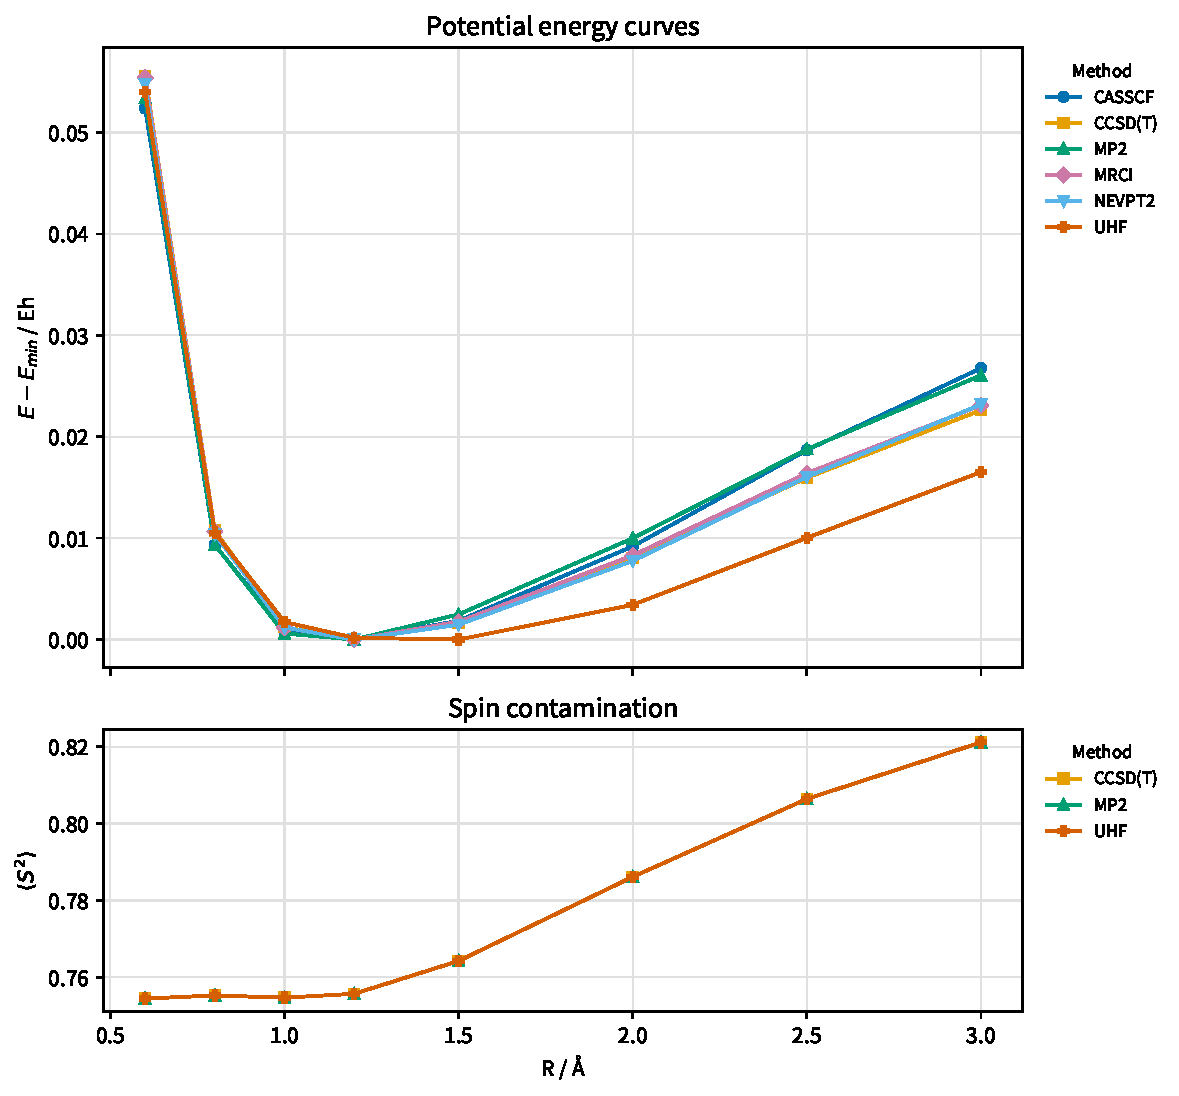
\includegraphics[width=\textwidth]{figures/ch07/h2m_pes.pdf}
\caption{H$_2^-$/def2-TZVPP 的势能曲线（上）与 UHF 的 $\langle S^2\rangle$（下）。
上图的纵轴是各方法自己的 $E-E_{\min}$，只用于比较曲线形状，不能跨方法比较绝对能量；
下图的 $\langle S^2\rangle$ 只由 UHF 参考给出，MP2 与 CCSD(T) 继承同一参考。}
\label{ch:07:fig:h2m}
\end{figure}

表~\ref{ch:07:tab:h2m} 把 UHF 与 CASSCF 的能量、UHF 的 $\langle S^2\rangle$ 以及 CASSCF 的活性空间自然占据数放在一起。最重要的数据事实是：CASSCF(3,2) 在\textbf{每一个} R 上都\textbf{高于} UHF，差值从 0.0012\,Eh（0.6\,\AA）到 0.0131\,Eh（3.0\,\AA）。这不表示 CASSCF“更差”。UHF 允许 $\alpha$ 与 $\beta$ 电子使用不同的空间轨道，变分自由度更大，代价是波函数不再是纯自旋本征态（$\langle S^2\rangle>0.75$）；CAS(3,2) 用两个共同的空间轨道并强制 \texttt{mult 2}，自旋是干净的，但能量会略高。用 CASSCF 与 UHF 的能量高低来判断“谁更可靠”是错误的，二者的变分空间与自旋约束不同。

\begin{table}[t]
\centering
\small
\caption{H$_2^-$/def2-TZVPP 的 UHF 与 CASSCF(3,2) 数据。能量单位 Eh，保留 6 位小数；
占据数取自 \texttt{data/h2m\_occupations.csv}，“偏离”指 $\min(|n_p|,|n_p-2|)$ 的最大值。
CASSCF 不打印 $\langle S^2\rangle$，因为 \texttt{mult 2} 已强制自旋本征态。}
\label{ch:07:tab:h2m}
\begin{tabular}{@{}lcccccc@{}}
\toprule
$R$/\AA & $E_{\mathrm{UHF}}$ & $E_{\mathrm{CASSCF}}$ & $\langle S^2\rangle_{\mathrm{UHF}}$ & $n_1$ & $n_2$ & 偏离 \\
\midrule
0.6 & $-0.934317$ & $-0.933069$ & 0.754473 & 2.0000 & 1.0000 & 1.0000 \\
0.8 & $-0.977755$ & $-0.976123$ & 0.755273 & 2.0000 & 1.0000 & 1.0000 \\
1.0 & $-0.986566$ & $-0.984600$ & 0.754710 & 2.0000 & 1.0000 & 1.0000 \\
1.2 & $-0.988117$ & $-0.985448$ & 0.755706 & 2.0000 & 1.0000 & 1.0000 \\
1.5 & $-0.988296$ & $-0.983600$ & 0.764251 & 2.0000 & 1.0000 & 1.0000 \\
2.0 & $-0.984874$ & $-0.976261$ & 0.786138 & 2.0000 & 1.0000 & 1.0000 \\
2.5 & $-0.978266$ & $-0.966776$ & 0.806405 & 2.0000 & 1.0000 & 1.0000 \\
3.0 & $-0.971787$ & $-0.958695$ & 0.821141 & 2.0000 & 1.0000 & 1.0000 \\
\bottomrule
\end{tabular}
\end{table}

表~\ref{ch:07:tab:h2m} 的占据数是本书必须诚实对待的地方。CAS(3,2) 的自然占据数在\textbf{所有} R 上都是 2.0000 与 1.0000，偏离恒为 1.0000；输出中的 CI 向量是单一组态（\texttt{1.00000 [1]:21}）。也就是说，\texttt{nroots 1} 的 CASSCF(3,2) 基态在这个最小活性空间里是一个\textbf{单一行列式}（在局域轨道表象中），并没有出现 1.5/1.5 那样的分数占据。占据数“偏离 0 或 2”之所以满足 1.0，只是因为单占据活性轨道的占据数本来就是 1.0，这不是分数静态相关的标志。

那么 H$_2^-$ 的多参考证据在哪里？在三处。第一，UHF 的 $\langle S^2\rangle$ 随 R 从 0.754473 增长到 0.821141，增长量 0.066668，远大于 0.02；自旋污染随键拉伸而加重，说明单参考自旋轨道图像在拉伸区失效（7.8 节）。第二，MP2 与 CCSD(T) 在拉伸区的行为异常：它们虽然仍给出更低的能量，但相对 CASSCF 的修正越来越大，且 CCSD(T) 的微扰分母在近简并时不可靠。第三，CASSCF 之上的 NEVPT2 与 MRCI 修正很大：NEVPT2 比 CASSCF 低 0.0331--0.0391\,Eh，MRCI 又比 NEVPT2 低 0.0129--0.0137\,Eh，且在每个 R 上都如此。动态相关修正的规模本身说明 CASSCF 参考态还远未完成，而 1.5/1.5 的静态相关图像必须由更大的活性空间或态平均计算才能显现，不能从这张表的单组态占据数里读出来。

\subsection{UHF 的自旋污染}
\label{ch:07:sec:spin}

H$_2^-$ 是双重态，纯自旋本征态的 $\langle S^2\rangle=0.75$。UHF 波函数不强制这一点，$\alpha$ 与 $\beta$ 轨道可以不同，于是 $\langle S^2\rangle$ 偏离 0.75。表~\ref{ch:07:tab:h2m} 与图~\ref{ch:07:fig:h2m} 的下半部分给出完整序列：0.754473（0.6\,\AA）、0.755273（0.8）、0.754710（1.0）、0.755706（1.2）、0.764251（1.5）、0.786138（2.0）、0.806405（2.5）、0.821141（3.0）。

这组数据有两个必须如实报告的细节。第一，增长不是严格单调的：0.8\,\AA 的 0.755273 比 1.0\,\AA 的 0.754710 高 0.000563，随后才继续上升。这个微小凹陷来自 SCF 收敛路径与轨道近简并的耦合，不影响“拉伸区污染加重”的结论，但不能为了叙事把它抹平。第二，0.75 附近的数值本身已经偏离纯自旋值，说明即使在平衡区附近，UHF 也不是纯双重态；只是到了 3.0\,\AA，偏离才明显放大。MP2 与 CCSD(T) 以 UHF 为参考，因此 CSV 中它们的 $S^2$ 列与 UHF 相同；这不是三个独立证据，而是同一个参考态的自旋污染被三种方法继承。

CASSCF 的情况不同：\texttt{mult 2} 强制波函数是自旋本征态，$\langle S^2\rangle$ 应为 0.75，ORCA 对这类计算不打印 $S^2$，CSV 中 CASSCF/NEVPT2/MRCI 的 $s^2$ 列为空。不能把“空”理解为“没有自旋污染”或“有污染”，它只是这些方法不输出该量；正确说法是自旋对称性由构造保证。

% ---- 4. CH4 结果框 ----
\begin{ch4box}
CH$_4$/def2-TZVPP：$E_{\mathrm{CASSCF}(8,8)} = -40.297163$\,Eh
（CSV 精确值 $-40.297162861153$\,Eh），
$\Delta E = +88.75$\,kcal·mol$^{-1}$（相对 CCSD(T)）。
活性空间自然占据数为 $1.98429$、$1.97895\times3$、$0.01971\times4$，总和 8。
这些数接近 2 与 0，说明 CH$_4$ 只有\textbf{弱}静态相关；它与拉伸 H$_2^-$ 的强近简并不是一回事。
CASSCF 缺掉的动态相关由第 8 章的 CASPT2/NEVPT2/MRCI 补上。
\end{ch4box}

% ---- 5. 常见陷阱 ----
\begin{pitfall}
\begin{itemize}
  \item \textbf{把 CASSCF 当成“自动包含所有相关”}：CASSCF 只包含活性空间内的静态相关；活性空间外的动态相关仍需 CASPT2、NEVPT2 或 MRCI。CASSCF 能量不能当作高精度基准。
  \item \textbf{用能量高低判断 CASSCF 与 UHF 谁更可靠}：UHF 的变分空间更大且允许自旋污染，能量更低并不代表波函数更好；比较必须看 $\langle S^2\rangle$、占据数与后续多参考修正。
  \item \textbf{把态平均结果当基态}：\texttt{nroots 2} 的态平均占据数可能是 1.5/1.5，但那是两个态的平均，不是 \texttt{nroots 1} 的基态；本书 H$_2^-$ 数据全部取 \texttt{nroots 1}。
  \item \textbf{活性空间越大越好}：式~\eqref{ch:07:eq:determinant-count} 的指数增长会让计算不可行；应先按化学直觉与占据数选最小空间，再做收敛性检查。
\end{itemize}
\end{pitfall}

% ---- 6. 小结 + 过渡 ----
\subsection*{小结}
CASSCF 用活性空间内的全 CI 式~\eqref{ch:07:eq:casscf-wavefunction} 容纳近简并组态，并通过式~\eqref{ch:07:eq:orbital-generator}--\eqref{ch:07:eq:orbital-ci-gradient} 把轨道与 CI 系数联合优化；它是变分的、尺寸一致的，但成本随活性空间指数增长（式~\eqref{ch:07:eq:determinant-count}）。H$_2^-$ 的 CAS(3,2) 数据给出了一个诚实的教训：\texttt{nroots 1} 的占据数是 2.0/1.0 而非 1.5/1.5，CASSCF 在能量上还高于 UHF，多参考必要性来自 $\langle S^2\rangle$ 增长与 NEVPT2/MRCI 的大修正，而不是 CASSCF--UHF 的能量排序。CASSCF 仍缺动态相关，这正是下一章要补的。带着这个问题，我们进入第 8 章：CASPT2/NEVPT2/MRCI：如何给多参考态补动态相关？

% ============================================================
% sections/ch08-mrpt-mrci.tex —— 第 8 章 CASPT2/NEVPT2/MRCI
% 页数配额：5 页（±1）。数值只取自 data/h2m_pes.csv 与 data/ch4_results.csv。
% ============================================================

\section{CASPT2/NEVPT2/MRCI：如何给多参考态补动态相关？}
\label{ch:08:sec:title}

% ---- 1. 问题链 ----
\begin{problemchain}
\textbf{上一章留下的问题：}CASSCF 缺动态相关。\\
\textbf{本章为什么存在：}多参考微扰（CASPT2/NEVPT2）与 MRCI 在 CASSCF 参考上补动态相关。\\
\textbf{本章留下的新问题：}成本高、活性空间选择难。
\end{problemchain}

% ---- 2. 方法卡片 ----
\begin{methodcard}
\textbf{方法}：$n$ 电子价态微扰理论（NEVPT2），并与 CASPT2、MRCI 对照\quad
\textbf{文献}：\citep{andersson1990,angeli2001,werner1988,knowles1988,lischka2018mr}\\
\textbf{核心近似}：CASSCF 参考 + 二阶微扰（CASPT2/NEVPT2）或单双激发组态展开（MRCI）\\
\textbf{关键方程}：式~\eqref{ch:08:eq:pt2-energy}（二阶微扰能量）\\
\textbf{ORCA 关键词}：\texttt{! NEVPT2 def2-TZVPP TightSCF}，
并在 \texttt{\%casscf} 中写 \texttt{nel 8 norb 8 mult 1 nroots 1}\\
\textbf{成本标度}：$\mathcal{O}(N^5)$ 乘以活性空间因子\\
\textbf{能否变分 / 尺寸一致}：否 / 是（PT2）；MRCI 变分但不尺寸一致\\
\textbf{典型失效}：CASPT2 的入侵态、活性空间依赖、MRCI 的尺寸不一致
\end{methodcard}

% ---- 3. 正文 ----
\subsection{CASPT2：零阶 Hamiltonian 与有效 Hamiltonian}
\label{ch:08:sec:caspt2}

第 7 章的 CASSCF 把静态相关收进活性空间，但活性空间外的动态相关仍被丢掉。最直接的做法是以 CASSCF 波函数为零阶参考，对剩余的激发空间做二阶微扰，这就是 CASPT2\citep{andersson1990}。把 Hamiltonian 分成零阶与微扰两部分：
\begin{equation}
\op{H}=\op{H}_0+\op{V},
\qquad
\op{H}_0=\op{P}\op{F}\op{P}+\op{Q}\op{F}\op{Q},
\label{ch:08:eq:partition}
\end{equation}
其中 $\op{P}$ 是 CASSCF 参考态及其活性空间组态张成的模型空间，$\op{Q}=1-\op{P}$ 是正交补，$\op{F}$ 是广义 Fock 算符。式~\eqref{ch:08:eq:partition} 的关键在于零阶 Hamiltonian 用 Fock 算符而非完整的 $\op{H}$：这样 $\op{H}_0$ 在 $\op{P}$ 与 $\op{Q}$ 内可对角化，微扰展开才有可计算的分母。

在二阶微扰下，有效 Hamiltonian 可以写成
\begin{equation}
\op{H}_{\mathrm{eff}}^{(2)}
=\op{P}\op{H}\op{P}
+\op{P}\op{V}\op{Q}\,
\frac{1}{E_0-\op{H}_0}\,
\op{Q}\op{V}\op{P},
\label{ch:08:eq:caspt2-effective}
\end{equation}
其中 $E_0$ 是零阶能量。式~\eqref{ch:08:eq:caspt2-effective} 把 CASSCF 模型空间内的相互作用与外部激发空间的二阶反馈合在一起；对角化它，就得到 CASPT2 对各个态的修正。对基态，二阶能量修正可写成更熟悉的形式：
\begin{equation}
E^{(2)}
=\sum_{K\notin P}
\frac{\big|\bracket{\Phi_K|\op{V}|\Psi_0}\big|^2}
     {E_0-E_K},
\label{ch:08:eq:pt2-energy}
\end{equation}
其中 $\ket{\Psi_0}$ 是 CASSCF 参考态，$\ket{\Phi_K}$ 与 $E_K$ 是 $\op{H}_0$ 在 $\op{Q}$ 空间的本征态与本征值。式~\eqref{ch:08:eq:pt2-energy} 与 MP2 的式~\eqref{ch:04:eq:mp2-energy} 形式相同，区别在参考态：这里的分母不再是 HF 轨道能差，而是 CASSCF 零阶能量与外部组态能量之差。

CASPT2 最著名的失效是\textbf{入侵态}（intruder state）：当某个外部组态的能量 $E_K$ 与 $E_0$ 近简并时，式~\eqref{ch:08:eq:pt2-energy} 的分母趋于零，修正发散或给出错误符号。实际计算常用 level shift 或 IPEA shift 把分母推开，但 shift 的数值会改变结果，必须报告。另一个问题是活性空间依赖：换一个 CAS，参考态与 $\op{Q}$ 空间都变，CASPT2 能量也随之变；因此 CASPT2 不是“选了 CASSCF 就自动可靠”，活性空间仍需做收敛性检查。

\subsection{NEVPT2：Dyall Hamiltonian 与无入侵态}
\label{ch:08:sec:nevpt2}

NEVPT2 换一个零阶 Hamiltonian 来消除入侵态\citep{angeli2001}。它使用 Dyall Hamiltonian：
\begin{equation}
\op{H}_D
=\sum_{i}\varepsilon_i\,\op{a}_i^\dagger\op{a}_i
+\sum_{a}\varepsilon_a\,\op{a}_a^\dagger\op{a}_a
+\op{H}_{\mathrm{act}},
\label{ch:08:eq:dyall}
\end{equation}
其中 $i$ 取非活性轨道，$a$ 取虚轨道，$\op{H}_{\mathrm{act}}$ 是只用活性空间积分构造的 CAS Hamiltonian。式~\eqref{ch:08:eq:dyall} 把非活性与虚轨道写成简单的单体形式，把全部多体效应留在活性空间内。这样做的直接后果是：$\op{H}_D$ 的本征值由活性空间的激发能加上非活性/虚轨道的轨道能差组成，分母有一个与活性空间能隙同量级的下界，不会出现 CASPT2 那种任意小的入侵态分母。

NEVPT2 的二阶能量按外部组态相对参考态的“空穴/粒子”数分类：
\begin{equation}
E_{\mathrm{NEVPT2}}
=E_{\mathrm{CAS}}^{(0)}
+\sum_{l=1}^{8}\sum_{K\in Q_l}
\frac{\big|\bracket{\Phi_K|\op{V}|\Psi_0}\big|^2}
     {E_0^{(0)}-E_K^{(0)}},
\label{ch:08:eq:nevpt2-energy}
\end{equation}
其中 $Q_l$ 是第 $l$ 类外部组态（$0h$、$1h$、$2h$ 等，共八类）。式~\eqref{ch:08:eq:nevpt2-energy} 的每一类都可以用活性空间的低阶密度矩阵收缩，因而成本可控；同时因为 $\op{H}_D$ 的分母有下界，NEVPT2 对入侵态是“免疫”的。代价是 NEVPT2 对零阶 Hamiltonian 的选择更刚性：它不像 CASPT2 那样可以通过 shift 调节，活性空间选得不好时结果仍会偏，只是不会以发散的形式表现出来。

\subsection{MRCI 与 Davidson 校正}
\label{ch:08:sec:mrci}

MRCI 走另一条路：不做微扰，而是直接把参考态周围的单、双激发组态加进波函数\citep{werner1988,knowles1988,lischka2018mr}。多参考 CI 波函数写成
\begin{equation}
\ket{\Psi_{\mathrm{MRCI}}}
=\sum_{I} c_I\ket{\Phi_I},
\label{ch:08:eq:mrci-wavefunction}
\end{equation}
其中 $\ket{\Phi_I}$ 包括参考组态以及它们相对于参考空间的单、双激发；$\op{H}$ 在展开空间内对角化，CI 系数由本征值问题定出。式~\eqref{ch:08:eq:mrci-wavefunction} 的参考可以是多个 CASSCF 组态，因此它能同时描述静态相关与相当一部分动态相关。若把参考空间取成完整的 CAS，再把单、双激发加到所有参考组态上，就得到常用的 CAS+SD 型 MRCI；内部收缩（internally contracted）实现把激发组合并，显著降低维数。

MRCI 是变分的，但截断到单、双激发后不尺寸一致：两个远离的片段各自做 MRCI，再放在一起做超体系 MRCI，能量不能严格相加。Davidson 提出一个后验修正来估计缺失的高阶激发\citep{langhoff1974}：
\begin{equation}
E_{\mathrm{Davidson}}
=E_{\mathrm{MRCI}}
+\Big(1-\sum_{I\in\mathrm{ref}}|c_I|^2\Big)
 \big(E_{\mathrm{MRCI}}-E_{\mathrm{ref}}\big),
\label{ch:08:eq:davidson}
\end{equation}
其中 $\sum_{I\in\mathrm{ref}}|c_I|^2$ 是参考组态在 MRCI 波函数中的总权重，$E_{\mathrm{ref}}$ 是参考态能量。式~\eqref{ch:08:eq:davidson} 的括号衡量“参考态被激发组态稀释了多少”；稀释越多，修正越大。Davidson 校正能改善解离能等性质，但它不是严格的尺寸一致修正，不能把 MRCI+Q 当作尺寸一致方法。

尺寸一致性的差别可以写成一个简单判据。对两个无相互作用的片段 $A$、$B$，
\begin{equation}
E_{AB}(R\to\infty)=E_A+E_B
\label{ch:08:eq:size-consistency}
\end{equation}
是任何尺寸一致方法必须满足的条件。CASPT2 与 NEVPT2 在各自的 CASSCF 参考满足该条件时继承式~\eqref{ch:08:eq:size-consistency}；截断 MRCI 不满足，Davidson 校正只是把它向式~\eqref{ch:08:eq:size-consistency} 拉近，并不恢复严格等式。这一点与第 5 章 CISD 的病根相同：线性截断丢了断开激发，只是 MRCI 的参考空间更大、误差通常更小。

\subsection{CASPT2、NEVPT2 与 MRCI 的比较}
\label{ch:08:sec:compare}

三种方法的分工可以用表~\ref{ch:08:tab:compare} 概括。CASPT2 的零阶 Hamiltonian 最灵活，能通过 shift 处理入侵态，但 shift 与活性空间都会影响结果；NEVPT2 用 Dyall Hamiltonian 换来无入侵态与更好的尺寸行为，代价是零阶选择更刚性；MRCI 是变分的、能直接给出波函数，但截断后不尺寸一致，成本也更高。实际选择通常取决于体系大小、是否需要激发态/性质、以及活性空间能否可靠确定。

\begin{table}[t]
\centering
\small
\caption{多参考动态相关方法的比较。活性空间因子对所有方法都存在；MRCI 的参考空间越大，其组态数增长越快。}
\label{ch:08:tab:compare}
\begin{tabular}{@{}lcccc@{}}
\toprule
方法 & 零阶/展开 & 入侵态 & 变分 & 尺寸一致 \\
\midrule
CASPT2 & CASSCF + 广义 Fock & 有 & 否 & 是 \\
NEVPT2 & Dyall Hamiltonian & 无 & 否 & 是 \\
MRCI & 参考 + 单双激发 & 无 & 是 & 否（+Q 近似） \\
CCSD(T) & 单参考 + 微扰三激发 & 有 & 否 & 是 \\
\bottomrule
\end{tabular}
\end{table}

表~\ref{ch:08:tab:compare} 中的“无”与“有”不是绝对的精度排序。MRCI 变分且参考空间大，常被当作多参考基准；但它的尺寸不一致会在键断裂、弱相互作用中显现。CASPT2 与 NEVPT2 非变分，能量可能低于或高于精确值；NEVPT2 的无入侵态优势不等于它对活性空间不敏感。三者都需要在相同活性空间、相同基组下比较，不能把不同 CAS 的绝对能量混在一起。

\subsection{H$_2^-$ 势能曲线：CASSCF、NEVPT2 与 MRCI}
\label{ch:08:sec:h2m-mr}

图~\ref{ch:08:fig:h2m-mr} 把 H$_2^-$/def2-TZVPP 的 CASSCF(3,2)、NEVPT2 与 MRCI 绝对能量画在一起。三条曲线的最低点都在 1.2\,\AA{} 附近：CASSCF 为 $-0.985448$\,Eh，NEVPT2 为 $-1.020944$\,Eh，MRCI 为 $-1.034539$\,Eh。NEVPT2 在每个 R 上都低于 CASSCF，差值 0.0331--0.0391\,Eh；MRCI 又在每个 R 上都低于 NEVPT2，差值 0.0129--0.0137\,Eh。这正是第 7 章留下的“缺动态相关”被补上的直接证据：CASSCF 参考之上的修正不仅大，而且在整条曲线上稳定存在。

\begin{figure}[t]
\centering
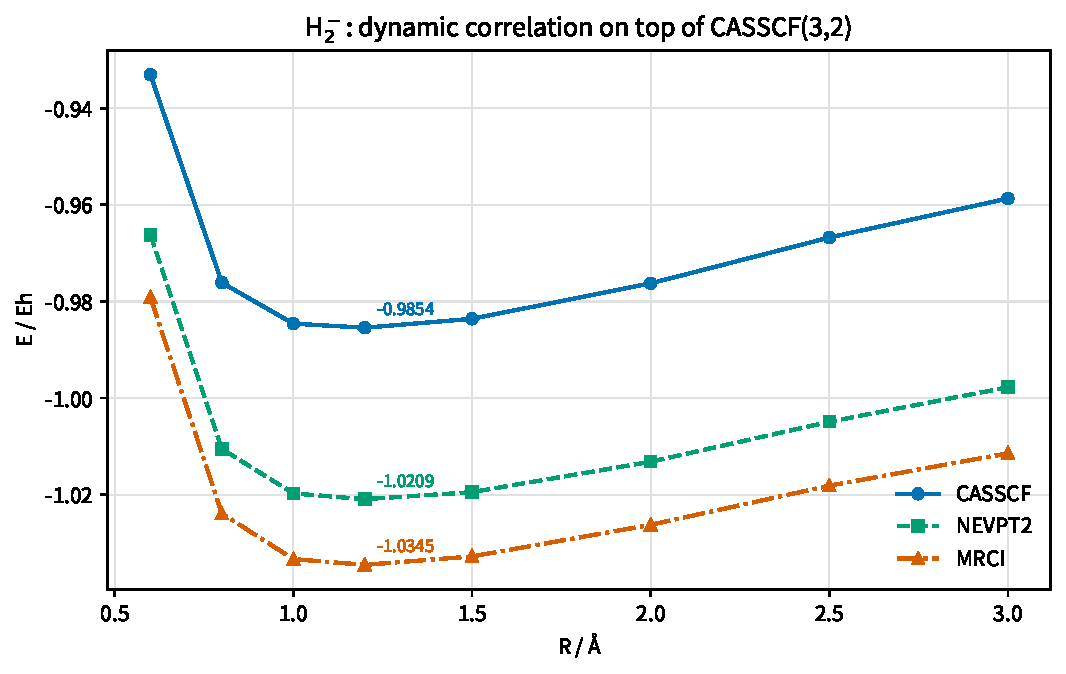
\includegraphics[width=0.86\textwidth]{figures/ch08/h2m_mr.pdf}
\caption{H$_2^-$/def2-TZVPP 的 CASSCF(3,2)、NEVPT2 与 MRCI 绝对能量（Eh）。
纵轴是绝对能量，因此可以直接看出三种方法在同一 R 上的相对位置；
三条曲线的最低点均在 $R=1.2$\,\AA{}。}
\label{ch:08:fig:h2m-mr}
\end{figure}

图~\ref{ch:08:fig:h2m-mr} 只画了三种方法，没有 CASPT2。原因不是 CASPT2 在物理上不适用，而是 ORCA 6.1.1 在 H$_2^-$/CAS(3,2) 的 CASPT2 清理阶段存在已知段错误\footnote{ORCA 6.1.1 在 H$_2^-$/CAS(3,2) 的 CASPT2 清理阶段存在已知段错误；本书因此不做 H$_2^-$ 的 CASPT2 扫描，CH$_4$ 的 CASPT2 数据来自 CAS(8,8) 计算。}。这是一个实现问题，不是 CASPT2 理论的失效；本书选择不伪造一条 CASPT2 曲线，而是用 NEVPT2 与 MRCI 展示多参考动态相关的效果。CASPT2 在 CH$_4$ 上的表现见下面的结果框。

\subsection{CH$_4$ 的 CAS(8,8) 结果与实现注记}
\label{ch:08:sec:ch4}

CH$_4$ 是弱静态相关体系，CAS(8,8) 的参考态已能描述其主要静态相关；在其上补动态相关，可以干净地比较三种方法。三种方法在 CH$_4$/def2-TZVPP 上给出的能量如下。CASPT2 为 $-40.420721$\,Eh，NEVPT2 为 $-40.405834$\,Eh，MRCI 为 $-40.428596$\,Eh；三者均低于 CASSCF 的 $-40.297163$\,Eh。MRCI 最低，CASPT2 次之，NEVPT2 再次；这与 H$_2^-$ 扫描中“NEVPT2 低于 CASSCF、MRCI 又低于 NEVPT2”的次序一致，说明动态相关修正的方向是稳定的。

但 CH$_4$ 的数值不能直接搬到 H$_2^-$ 上。H$_2^-$ 的 CAS(3,2) 是一个极小的活性空间，NEVPT2 与 MRCI 的修正主要来自活性空间外的动态相关；CH$_4$ 的 CAS(8,8) 已包含更多价相关，剩余修正较小。两者都说明 CASSCF 不是终点，但修正的绝对大小依赖活性空间。CASPT2 在 CH$_4$ 上能正常完成，正说明 8.5 节缺失的 H$_2^-$ CASPT2 曲线是 ORCA 对该特定体系/活性空间的清理 bug，而不是方法本身的普遍问题。

% ---- 4. CH4 结果框 ----
\begin{ch4box}
CH$_4$/def2-TZVPP：$E_{\mathrm{CASPT2}} = -40.420721$\,Eh
（CSV 精确值 $-40.420720703026$\,Eh），
$\Delta E = +11.22$\,kcal·mol$^{-1}$；
$E_{\mathrm{NEVPT2}} = -40.405834$\,Eh
（CSV 精确值 $-40.405833810464$\,Eh），
$\Delta E = +20.56$\,kcal·mol$^{-1}$；
$E_{\mathrm{MRCI}} = -40.428596$\,Eh
（CSV 精确值 $-40.428596004396$\,Eh），
$\Delta E = +6.28$\,kcal·mol$^{-1}$。
参考值为 CCSD(T) 的 $-40.438598$\,Eh。
在 CH$_4$ 上按能量从低到高为 MRCI、CASPT2、NEVPT2、CASSCF，
与 H$_2^-$ 扫描中 MRCI $<$ NEVPT2 $<$ CASSCF 的次序一致。
\end{ch4box}

% ---- 5. 常见陷阱 ----
\begin{pitfall}
\begin{itemize}
  \item \textbf{把 CASPT2 当作黑箱}：式~\eqref{ch:08:eq:pt2-energy} 的分母可能被入侵态击穿；level shift/IPEA shift 的取值会改变能量，必须与活性空间一起报告。
  \item \textbf{认为 NEVPT2 对活性空间不敏感}：Dyall Hamiltonian 只保证分母有下界，不保证结果与活性空间无关；式~\eqref{ch:08:eq:nevpt2-energy} 仍依赖 CAS 的选择。
  \item \textbf{把 MRCI 当尺寸一致方法}：MRCI 变分但不满足式~\eqref{ch:08:eq:size-consistency}；Davidson 校正式~\eqref{ch:08:eq:davidson} 只是近似补救，不是严格修正。
  \item \textbf{跨活性空间比较绝对能量}：CASPT2/NEVPT2/MRCI 的能量都建立在特定 CAS 上；换活性空间就是换参考态，绝对能量不可直接对比。
\end{itemize}
\end{pitfall}

% ---- 6. 小结 + 过渡 ----
\subsection*{小结}
CASPT2 用式~\eqref{ch:08:eq:caspt2-effective}--\eqref{ch:08:eq:pt2-energy} 在 CASSCF 参考上做二阶微扰，能补动态相关但受入侵态与 shift 影响；NEVPT2 用 Dyall Hamiltonian 式~\eqref{ch:08:eq:dyall} 消除入侵态，并按式~\eqref{ch:08:eq:nevpt2-energy} 分类求和；MRCI 用式~\eqref{ch:08:eq:mrci-wavefunction} 直接展开单双激发，变分但不尺寸一致，Davidson 校正只是近似。H$_2^-$ 扫描中 NEVPT2 与 MRCI 在每个 R 上都低于 CASSCF，CH$_4$ 上 MRCI 最低、CASPT2 次之、NEVPT2 再次、CASSCF 最高，二者共同说明多参考动态相关修正的方向稳定，但成本与活性空间选择仍是实际瓶颈。带着这个问题，我们进入第 9 章：DFT：能不能不写波函数？

\section{DFT：能不能不写波函数？}
\label{ch:09:sec:title}
% TODO(T7/T8/...): 本章由后续写作任务填充；数值只取自 data/*.csv。

% ============================================================
% sections/ch10-lda-gga.tex —— 第 10 章 LDA/GGA：密度泛函前两级够用吗？
% 页数配额：6 页（±1）。数值只取自 data/*.csv。
% ============================================================

\section{LDA/GGA：密度泛函前两级够用吗？}
\label{ch:10:sec:title}

% ---- 1. 问题链 ----
\begin{problemchain}
\textbf{上一章留下的问题：}$E_\xc$ 泛函未知。\\
\textbf{本章为什么存在：}用均匀电子气（LDA）与密度梯度（GGA）近似 $E_\xc$，把第 9 章的 KS 框架变成可实际计算的泛函。\\
\textbf{本章留下的新问题：}仍半局域、自相互作用误差、无色散、带隙低估。
\end{problemchain}

% ---- 2. 方法卡片 ----
\begin{methodcard}
\textbf{方法}：局域密度近似（LDA，ORCA 中为 SVWN5）与广义梯度近似（GGA，以 PBE 为代表）\quad
\textbf{文献}：\citep{vosko1980,ceperley1980,perdew1981sie,becke1988,lee1988,perdew1996pbe}\\
\textbf{核心近似}：$E_\xc$ 只依赖局域密度 $\rho(\mathbf r)$（LDA）或再依赖密度梯度 $\nabla\rho(\mathbf r)$（GGA），即半局域近似。\\
\textbf{关键方程}：式~\eqref{ch:10:eq:gga-enhancement}（PBE 增强因子）\\
\textbf{ORCA 关键词}：\texttt{! PBE def2-TZVPP TightSCF}（LDA 用 \texttt{! LDA}，ORCA 取 SVWN5）\\
\textbf{成本标度}：$\mathcal{O}(N^3)$\quad
\textbf{能否变分 / 尺寸一致}：对给定泛函可变分；尺寸一致且广延。\\
\textbf{典型失效}：过 binding、无色散、带隙低估；B97-3c 是复合方法，不是新梯级。
\end{methodcard}

% ---- 3. 正文 ----
\subsection{均匀电子气与局域密度近似}
\label{ch:10:sec:lda}

第 9 章把 DFT 的全部困难压缩成一个未知泛函 $E_\xc[\rho]$。最自然的出发点是\textbf{均匀电子气}（uniform electron gas）：电子在均匀正电荷背景中运动，密度处处为常数，交换相关能可以高精度求出。LDA 的假设是：在空间每一点 $\mathbf r$，交换相关能密度等于密度为 $\rho(\mathbf r)$ 的均匀电子气的结果，
\begin{equation}
E_\xc^{\mathrm{LDA}}[\rho]
= \int \rho(\mathbf r)\,\varepsilon_\xc^{\mathrm{unif}}\big(\rho(\mathbf r)\big)\,\dd\mathbf r .
\label{ch:10:eq:lda-energy}
\end{equation}
式~\eqref{ch:10:eq:lda-energy} 只使用一点的密度，因此称为\textbf{局域}近似；对自旋极化的情形，把 $\varepsilon_\xc^{\mathrm{unif}}$ 写成 $\rho_\alpha$ 与 $\rho_\beta$ 的函数即可（LSDA）。实际使用的 SVWN5 由 Slater 交换与 VWN5 相关组成：交换部分取均匀电子气的解析结果，相关部分用 Vosko--Wilk--Nusair 对 Ceperley--Alder 量子蒙特卡罗数据的拟合\citep{vosko1980,ceperley1980,perdew1981sie}。ORCA 的 \texttt{! LDA} 关键词即对应这一组合。

LDA 在均匀或近均匀体系（简单金属、价电子较离域的固体）中表现不错，但分子中的密度远非均匀：原子核附近密度高、化学键区域密度变化剧烈、远尾指数衰减。把每一点当作均匀电子气，等于忽略了这些梯度信息，这正是下一节 GGA 要修补的地方。

\subsection{LDA 交换能与交换势}
\label{ch:10:sec:lda-exchange}

均匀电子气的交换能密度可以解析求出。对闭壳层体系，
\begin{equation}
E_x^{\mathrm{LDA}}[\rho]
= -C_x\int \rho(\mathbf r)^{4/3}\,\dd\mathbf r,
\qquad
C_x=\frac{3}{4}\Big(\frac{3}{\pi}\Big)^{1/3}\approx 0.7386 .
\label{ch:10:eq:lda-exchange}
\end{equation}
式~\eqref{ch:10:eq:lda-exchange} 就是 Slater 交换能；对开壳层体系，把积分拆成自旋分量 $\sum_\sigma\int\rho_\sigma^{4/3}\,\dd\mathbf r$，即 LSDA。它的形式极其简单：交换能只与 $\rho^{4/3}$ 的积分有关，没有任何梯度或非局域信息。

相关部分没有解析闭式，SVWN5 采用 VWN5 参数化。写成自旋极化形式，
\begin{equation}
E_c^{\mathrm{LDA}}[\rho_\alpha,\rho_\beta]
= \int \rho(\mathbf r)\,\varepsilon_c^{\mathrm{VWN}}\big(r_s(\mathbf r),\zeta(\mathbf r)\big)\,\dd\mathbf r,
\qquad
r_s=\Big(\frac{3}{4\pi\rho}\Big)^{1/3},
\quad
\zeta=\frac{\rho_\alpha-\rho_\beta}{\rho},
\label{ch:10:eq:lda-correlation}
\end{equation}
其中 $r_s$ 是 Wigner--Seitz 半径，$\zeta$ 是自旋极化率。VWN5 在 $r_s\to 0$ 与 $r_s\to\infty$ 的渐近行为之间做插值，并拟合 Ceperley--Alder 的数值结果\citep{vosko1980,ceperley1980}。相关能通常只占总能量的很小一部分，但化学精度要求的正是这一小部分，因此相关泛函的参数化细节很重要。

对式~\eqref{ch:10:eq:lda-exchange} 做泛函导数，得到 LDA 交换势
\begin{equation}
v_x^{\mathrm{LDA}}(\mathbf r)
= \frac{\delta E_x^{\mathrm{LDA}}}{\delta\rho(\mathbf r)}
= -\frac{4}{3}C_x\,\rho(\mathbf r)^{1/3}.
\label{ch:10:eq:lda-potential}
\end{equation}
式~\eqref{ch:10:eq:lda-potential} 在均匀电子气中是精确的，但用于分子时有一个致命后果：一个电子在自身的库仑势中仍然感受到交换势的抵消不完整，即\textbf{自相互作用误差}（self-interaction error，SIE）。对氢原子，精确的交换相关能应当恰好抵消电子与自身的库仑排斥；LDA 只能抵消一部分，剩余部分使电子过度离域。这个误差会传播到电荷转移能、反应能垒与带隙，是后续杂化泛函（第 12 章）要处理的核心问题。

\subsection{梯度展开与 GGA 交换}
\label{ch:10:sec:gga}

LDA 忽略密度变化，最直接的改进是把梯度加进来。定义无量纲的约化密度梯度
\begin{equation}
s(\mathbf r)=\frac{\lvert\nabla\rho(\mathbf r)\rvert}{2k_F(\mathbf r)\,\rho(\mathbf r)},
\qquad
k_F=(3\pi^2\rho)^{1/3},
\label{ch:10:eq:reduced-gradient}
\end{equation}
其中 $k_F$ 是局域费米波矢。$s$ 衡量密度在费米波长尺度上变化的快慢：$s=0$ 对应均匀电子气，$s$ 越大表示越不均匀。GGA 交换能写成
\begin{equation}
E_x^{\mathrm{GGA}}[\rho]
= \int \rho(\mathbf r)\,\varepsilon_x^{\mathrm{unif}}\big(\rho(\mathbf r)\big)\,
F_x\big(s(\mathbf r)\big)\,\dd\mathbf r ,
\label{ch:10:eq:gga-exchange}
\end{equation}
其中 $\varepsilon_x^{\mathrm{unif}}(\rho)=-C_x\rho^{1/3}$ 是均匀电子气的交换能密度，$F_x(s)$ 称为\textbf{增强因子}（enhancement factor）。式~\eqref{ch:10:eq:gga-exchange} 的结构说明：GGA 仍然以 LDA 为底，只用一个标量函数 $F_x(s)$ 调制它。不同的 GGA 差别几乎全在 $F_x(s)$ 的形状上。

最简单的梯度展开给出 $F_x(s)=1+\mu_{\mathrm{GE}}s^2+\cdots$，其中 $\mu_{\mathrm{GE}}=10/81\approx 0.1235$。这个展开只在小 $s$ 极限可靠；在分子中 $s$ 可以很大，直接截断会破坏交换能的渐近行为。Becke 与 Lee--Yang--Parr 的 GGA 分别从不同经验或约束条件构造 $F_x$ 与相关泛函\citep{becke1988,lee1988}；PBE 则选择尽量满足已知精确约束的形式\citep{perdew1996pbe}。

\subsection{PBE 增强因子与相关泛函}
\label{ch:10:sec:pbe}

PBE 交换增强因子取一个有理函数形式，
\begin{equation}
F_x^{\mathrm{PBE}}(s)
= 1+\kappa-\frac{\kappa}{1+\mu s^2/\kappa},
\qquad
\kappa=0.804,\quad \mu=0.21951 .
\label{ch:10:eq:gga-enhancement}
\end{equation}
式~\eqref{ch:10:eq:gga-enhancement} 的两个参数各有来历：$\mu$ 由线性响应恢复梯度展开系数（PBE 取 $\mu=\beta\pi^2/3$，$\beta=0.066725$），$\kappa$ 控制大 $s$ 的饱和值，使交换能不超过 Lieb--Oxford 上界。它的两个极限是
\begin{equation}
\lim_{s\to 0}F_x^{\mathrm{PBE}}(s)=1,
\qquad
\lim_{s\to\infty}F_x^{\mathrm{PBE}}(s)=1+\kappa\approx 1.804 .
\label{ch:10:eq:enhancement-limits}
\end{equation}
式~\eqref{ch:10:eq:enhancement-limits} 说明 PBE 在均匀极限回到 LDA，在强不均匀区域饱和而不是发散；这正是它比裸梯度展开稳健的原因。$\kappa$ 与 $\mu$ 不是拟合分子数据得到的，而是由约束确定的，因此 PBE 是一个"非经验"GGA。

PBE 的相关泛函在 LDA 相关能上再加一个梯度修正项：
\begin{equation}
\begin{aligned}
E_c^{\mathrm{PBE}}[\rho]
&= \int \rho(\mathbf r)\Big[\varepsilon_c^{\mathrm{unif}}\big(r_s,\zeta\big)
+ H\big(r_s,\zeta,t\big)\Big]\,\dd\mathbf r,\\
H&= \gamma\phi^3\ln\!\left\{1+\frac{\beta}{\gamma}\,t^2\,
\frac{1+At^2}{1+At^2+A^2t^4}\right\},
\end{aligned}
\label{ch:10:eq:pbe-correlation}
\end{equation}
其中 $t=\lvert\nabla\rho\rvert/(2\phi k_s\rho)$，$k_s=(4k_F/\pi)^{1/2}$，$\phi=\tfrac12[(1+\zeta)^{2/3}+(1-\zeta)^{2/3}]$，$\gamma=(1-\ln 2)/\pi^2\approx 0.031091$，$A=(\beta/\gamma)[\exp(-\varepsilon_c^{\mathrm{unif}}/(\gamma\phi^3))-1]^{-1}$。式~\eqref{ch:10:eq:pbe-correlation} 保证在 $t\to 0$ 时回到 LDA 相关能，并在大 $t$ 时给出正确的渐近行为。交换与相关合起来，PBE 只有两个可调参数 $\beta$ 与 $\kappa$（后者由约束固定），这也是它被广泛用作默认 GGA 的原因。

\subsection{B97-3c：复合方法，不是新梯级}
\label{ch:10:sec:b973c}

B97-3c 常被误认为"比 GGA 更高一级的泛函"。事实上它是一个\textbf{复合方法}（composite method）：以 B97 GGA 为电子结构核心，配上内置的 def2-mTZVP 基组、D3(BJ) 色散校正与短程基组（SRB）校正。D3(BJ) 的能量形式为
\begin{equation}
E_{D3(\mathrm{BJ})}
= -\frac12\sum_{A\neq B}\left[
\frac{s_6\,C_6^{AB}}{R_{AB}^6+(a_1R_{AB}^0+a_2)^6}
+\frac{s_8\,C_8^{AB}}{R_{AB}^8+(a_1R_{AB}^0+a_2)^8}
\right],
\label{ch:10:eq:d3bj}
\end{equation}
其中 $C_6^{AB}$、$C_8^{AB}$ 是原子对色散系数，$R_{AB}^0$ 是截断半径，$a_1,a_2$ 是阻尼参数\citep{grimme2010d3,grimme2011d3bj}。式~\eqref{ch:10:eq:d3bj} 是纯几何的加和，不改变 KS 方程，只把长程相关以经验方式补回。

于是 B97-3c 的总能可示意为
\begin{equation}
E_{\mathrm{B97}\text{-}\mathrm{3c}}
= E_\xc^{\mathrm{B97}}[\rho]
+ E_{D3(\mathrm{BJ})}
+ E_{\mathrm{SRB}}
+ E_{\mathrm{nuc}},
\label{ch:10:eq:b973c-energy}
\end{equation}
其中 $E_{\mathrm{SRB}}$ 是短程基组校正，用来补偿小基组带来的基组叠加误差；$E_{\mathrm{nuc}}$ 是核排斥能。式~\eqref{ch:10:eq:b973c-energy} 表明 B97-3c 的"3c"指三层校正（泛函、基组、色散/短程），而不是雅各布天梯上的第三个梯级。它使用的是内置 def2-mTZVP，不能写成 def2-TZVPP，也不能与同基组的 GGA 逐项比较绝对能量\citep{brandenburg2018b973c}。本书把 B97-3c 放在 GGA 一节讨论，是因为它的电子结构核心仍是 GGA；它是\textbf{复合方法，非新 rung}。

\subsection{数值积分与网格}
\label{ch:10:sec:grid}

DFT 的交换相关能是三维积分，实际计算用数值求积：
\begin{equation}
\int f(\mathbf r)\,\dd\mathbf r
\approx \sum_A \sum_{i\in A}
\frac{P_A(\mathbf r_i)}{\sum_B P_B(\mathbf r_i)}\,
\omega_i^{(A)}\,f(\mathbf r_i),
\label{ch:10:eq:grid-quadrature}
\end{equation}
其中 $P_A$ 是以原子 $A$ 为中心的 Becke 权重函数，$\omega_i^{(A)}$ 是原子 $A$ 的径向--角向求积权重（含径向 Jacobian）。式~\eqref{ch:10:eq:grid-quadrature} 就是 Becke 分块（fuzzy cells）：把分子空间划分成以各原子为中心的模糊胞，再在每个胞内用径向--角向网格积分。径向常用 Gauss--Chebyshev 或 Euler--Maclaurin 变换，角向常用 Lebedev 网格。LDA 与 GGA 的被积函数较平滑，中等网格即可收敛；meta-GGA（第 11 章）含动能密度，被积函数对网格更敏感，这是下一章要强调的数值问题。

\subsection{LDA/GGA 的失效模式}
\label{ch:10:sec:failures}

LDA 与 GGA 的误差有清楚的物理来源，可归纳为四类。第一，\textbf{过度结合（overbinding）}：半局域泛函倾向于把电子云拉得更近，键能偏大、平衡键长偏短；LDA 最明显，GGA 有所改善但仍未根除。第二，\textbf{无色散}：$\rho$ 与 $\nabla\rho$ 都是局域量，无法描述两个远离分子间的长程相关，稀有气体二聚体与 $\pi$--$\pi$ 堆积在纯 GGA 下几乎不结合；式~\eqref{ch:10:eq:d3bj} 的 D3 校正正是为此加入的经验补丁。第三，\textbf{带隙低估}：精确 $E_\xc$ 在粒子数改变时存在导数不连续，半局域泛函把它抹平，导致 HOMO--LUMO 隙偏小；SIE 又使电子过度离域，进一步压低带隙。第四，\textbf{自相互作用误差}：式~\eqref{ch:10:eq:lda-potential} 的交换势不能完全抵消电子与自身的库仑作用，造成电荷转移能与反应能垒的系统误差。

这些失效不是"参数没调好"，而是半局域近似的结构性限制：只使用 $\rho$ 与 $\nabla\rho$ 的泛函无法同时满足所有精确约束。沿雅各布天梯上行有两条路：加入动能密度 $\tau$（第 11 章 meta-GGA），或混入精确交换（第 12 章杂化）。两条路都只能缓解、不能消除 SIE；彻底处理非局域相关需要双杂化（第 13 章）或波函数方法。

% ---- 4. CH4 结果框 ----
\begin{ch4box}
CH$_4$ 单点，ORCA 关键词分别为 \texttt{! LDA def2-TZVPP TightSCF}、\texttt{! PBE def2-TZVPP TightSCF} 与 \texttt{! B97-3c TightSCF}。表~\ref{ch:10:tab:ch4} 给出三个泛函的总能与相对 CCSD(T)/def2-TZVPP 的偏差。

\begin{center}
\small
\begin{tabular}{@{}llrr@{}}
\toprule
方法 & 基组 & $E$ / Eh & $\Delta E$ / (kcal·mol$^{-1}$) \\
\midrule
SVWN5（LDA） & def2-TZVPP & $-40.117774$ & $+201.32$ \\
PBE（GGA）   & def2-TZVPP & $-40.464324$ & $-16.14$ \\
B97-3c       & def2-mTZVP（内置） & $-40.497380$ & $-36.89$ \\
\midrule
CCSD(T)（参考） & def2-TZVPP & $-40.438598$ & $0.00$ \\
\bottomrule
\end{tabular}
\captionof{table}{CH$_4$/def2-TZVPP 下 SVWN5、PBE 与 B97-3c 的总能及相对 CCSD(T) 的偏差；B97-3c 使用内置 def2-mTZVP。}
\label{ch:10:tab:ch4}
\end{center}

以 PBE 为例，$\Delta E=(-40.464324+40.438598)\times 627.509474=-16.14$\,kcal·mol$^{-1}$；用未舍入的 CSV 能量计算得 $-16.143346$。SVWN5 的 $+201.32$ 与 B97-3c 的 $-36.89$ 同理由 CSV 精确值换算。B97-3c 使用内置 def2-mTZVP 并含 D3(BJ) 与 SRB 校正，因此它的 $\Delta E$ 同时包含泛函、基组与色散修正的贡献，不能解释为"B97-3c 比 PBE 更准"。
\end{ch4box}

% ---- 5. 常见陷阱 ----
\begin{pitfall}
\begin{itemize}
  \item \textbf{把总能量更低当作更准}：PBE 的 $-40.464324$\,Eh 比 CCSD(T) 低约 $0.0257$\,Eh，这是泛函的系统偏移；$\Delta E$ 的正负号只表示相对参考的高低，不表示"更好"。
  \item \textbf{把 B97-3c 当作新梯级}：B97-3c 是 GGA + 内置基组 + D3(BJ)/SRB 的复合方法，不是雅各布天梯的第三级；把它与 def2-TZVPP 的 PBE 直接比较总能量会混淆基组效应。
  \item \textbf{用粗网格评估 meta-GGA}：式~\eqref{ch:10:eq:grid-quadrature} 的求积误差在 LDA/GGA 上较小，但对含 $\tau$ 的泛函可能达到 kcal·mol$^{-1}$ 量级；换泛函时必须同时检查网格。
\end{itemize}
\end{pitfall}

% ---- 6. 小结 + 过渡 ----
\subsection*{小结}
本章沿雅各布天梯爬了前两级。LDA 把每一点的交换相关能取为均匀电子气的结果，见式~\eqref{ch:10:eq:lda-energy}；交换能由式~\eqref{ch:10:eq:lda-exchange} 给出；相关能用 VWN5 参数化，见式~\eqref{ch:10:eq:lda-correlation}；交换势为式~\eqref{ch:10:eq:lda-potential}。GGA 引入约化梯度 $s$，见式~\eqref{ch:10:eq:reduced-gradient}；它用增强因子调制 LDA 交换，见式~\eqref{ch:10:eq:gga-exchange}。PBE 的 $F_x(s)$ 由式~\eqref{ch:10:eq:gga-enhancement} 给出，极限由式~\eqref{ch:10:eq:enhancement-limits} 固定，相关修正为式~\eqref{ch:10:eq:pbe-correlation}。B97-3c 是复合方法而非新梯级，其总能量见式~\eqref{ch:10:eq:b973c-energy}，其中包含 GGA、内置基组与 D3(BJ)（式~\eqref{ch:10:eq:d3bj}）。数值实现依赖式~\eqref{ch:10:eq:grid-quadrature} 的网格求积。遗憾的是，LDA/GGA 仍是半局域泛函：SIE、缺色散与带隙低估都还在。能不能只再加一个局域量——动能密度——就把这些问题改善？带着这个问题，我们进入第 11 章：meta-GGA：加入动能密度能解决什么？

\section{meta-GGA：加入动能密度能解决什么？}
\label{ch:11:sec:title}
% TODO(T7/T8/...): 本章由后续写作任务填充；数值只取自 data/*.csv。

% ============================================================
% sections/ch12-hybrid.tex —— 第 12 章 杂化：精确交换能修正什么？
% 页数配额：5 页（±1）。数值只取自 data/ch4_results.csv。
% ============================================================

\section{杂化：精确交换能修正什么？}
\label{ch:12:sec:title}

% ---- 1. 问题链 ----
\begin{problemchain}
\textbf{上一章留下的问题：}meta-GGA 仍有 SIE、缺非局域相关。\\
\textbf{本章为什么存在：}混入精确交换（全局或范围分离）可以部分抵消自相互作用，并修正交换势的渐近行为。\\
\textbf{本章留下的新问题：}仍缺动态相关。
\end{problemchain}

% ---- 2. 方法卡片 ----
\begin{methodcard}
\textbf{方法}：杂化泛函（hybrid functional），代表 B3LYP 与 $\omega$B97M-V\quad
\textbf{文献}：\citep{becke1993b3lyp,lee1988,adamo1999pbe0,mardirossian2016wb97mv}\\
\textbf{核心近似}：用一部分精确（HF 型）交换替换半局域交换；$\omega$B97M-V 还使用范围分离与 VV10 非局域相关\\
\textbf{关键方程}：式~\eqref{ch:12:eq:global-hybrid}\\
\textbf{ORCA 关键词}：\texttt{! B3LYP def2-TZVPP TightSCF}；\texttt{! wB97M-V def2-TZVPP TightSCF}\\
\textbf{成本标度}：$\mathcal{O}(N^4)$\quad
\textbf{能否变分 / 尺寸一致}：是 / 是（精确交换使泛函依赖轨道，按广义 KS 处理）\\
\textbf{典型失效}：强静态相关、SIE 只被部分消除、色散仍需 D3 等校正
\end{methodcard}

% ---- 3. 正文 ----
\subsection{自相互作用误差（SIE）}
\label{ch:12:sec:sie}

第 9 章把 DFT 的全部近似压缩进交换相关泛函 $E_\xc[\rho]$，第 10--11 章逐级加入密度梯度与动能密度——从 PBE\citep{perdew1996pbe} 到 TPSS\citep{tao2003}——但半局域泛函始终只“看见”局部的密度信息。这种半局域性最直接的后果是\textbf{自相互作用误差}（self-interaction error，SIE）：一个电子与自身的库仑排斥没有被交换项完全抵消\citep{perdew1981sie}。

考虑只含一个电子的密度 $\rho_1(\mathbf r)=\lvert\phi_1(\mathbf r)\rvert^2$。真实系统没有电子--电子相互作用，因此 Hartree 能必须被交换能精确抵消，相关能为零。对单电子密度，精确交换满足 $E_x^{\HF}[\rho_1]=-E_{\mathrm H}[\rho_1]$；任何近似泛函若做不到这一点，就留下非零的残余：
\begin{equation}
\Delta_{\mathrm{SIE}}[\rho_1]
= E_{\mathrm H}[\rho_1] + E_\xc[\rho_1] \neq 0,
\qquad
E_{\mathrm H}[\rho_1]
= \frac{1}{2}\iint
\frac{\rho_1(\mathbf r)\,\rho_1(\mathbf r')}
{\lvert\mathbf r-\mathbf r'\rvert}
\,\dd\mathbf r\,\dd\mathbf r'.
\label{ch:12:eq:sie}
\end{equation}
式~\eqref{ch:12:eq:sie} 是 SIE 的定义。对 LDA 与 GGA，$E_{\mathrm H}$ 中的自库仑项远大于近似的交换项，残余为正值；电子因此“讨厌自己”，倾向于把密度摊开。后果包括分数电荷能量偏离分段线性、电荷转移激发能低估、反应能垒偏低，以及自由基与过渡金属体系的自旋密度分布错误。

精确交换能按定义抵消单电子的全部自库仑项。若在泛函中混入比例为 $a_x$ 的精确交换，则到一阶近似，残余 SIE 按同一比例缩小：
\begin{equation}
\Delta_{\mathrm{SIE}}^{\mathrm{hybrid}}(a_x)
\approx (1-a_x)\,\Delta_{\mathrm{SIE}}^{\mathrm{DFT}}.
\label{ch:12:eq:sie-hybrid}
\end{equation}
式~\eqref{ch:12:eq:sie-hybrid} 说明了杂化泛函“修正什么”：它并不是新的相关泛函，而是用非局域的精确交换替换掉一部分有自相互作用的半局域交换。需要强调，这里的“精确交换”是用当前（广义）KS 轨道计算的 HF 型交换能，而不是第 3 章在 HF 轨道上算出的交换能；轨道随泛函一起自洽优化。

\subsection{全局杂化：B3LYP}
\label{ch:12:sec:global}

最简单的混合方式是在所有电子间距离上使用同一个精确交换比例，称为\textbf{全局杂化}（global hybrid）：
\begin{equation}
E_\xc
= a_x E_x^{\HF}
+ (1-a_x)\,E_x^{\mathrm{DFT}}
+ E_c^{\mathrm{DFT}}.
\label{ch:12:eq:global-hybrid}
\end{equation}
式~\eqref{ch:12:eq:global-hybrid} 中 $a_x$ 是精确交换分数，$E_x^{\mathrm{DFT}}$ 与 $E_c^{\mathrm{DFT}}$ 是半局域交换与相关。$a_x=0$ 退化为普通 GGA/meta-GGA，$a_x=1$ 则交换全部精确、相关仍用 DFT。由于精确交换是轨道泛函，式~\eqref{ch:12:eq:global-hybrid} 的能量不能写成密度的简单泛函；实际求解的是广义 Kohn--Sham（generalized KS，GKS）方程，交换势取轨道泛函的导数。

B3LYP 是最著名的全局杂化\citep{becke1993b3lyp,lee1988}。它把 Becke 三参数交换与 LYP 相关组合起来：
\begin{equation}
E_\xc^{\mathrm{B3LYP}}
= 0.20\,E_x^{\HF}
+ 0.80\,E_x^{\mathrm{LDA}}
+ 0.72\,\Delta E_x^{\mathrm{B88}}
+ 0.81\,E_c^{\mathrm{LYP}}
+ 0.19\,E_c^{\mathrm{VWN5}},
\label{ch:12:eq:b3lyp}
\end{equation}
其中 $\Delta E_x^{\mathrm{B88}}=E_x^{\mathrm{B88}}-E_x^{\mathrm{LDA}}$ 是 B88 梯度修正，$E_c^{\mathrm{VWN5}}$ 是 VWN5 局域相关。式~\eqref{ch:12:eq:b3lyp} 的三个系数 $(0.20,0.72,0.81)$ 是 1993 年针对热化学数据库拟合的，精确交换分数 $a_x=0.20$ 并非从第一原理导出。PBE0 则取 $a_x=1/4$，这个分数可由微扰论论证，因而被视为“无参数”杂化\citep{adamo1999pbe0}。两者都只用一个全局比例，无法同时优化短程与长程行为：20\%--25\% 的精确交换足以缓解价区的 SIE，却不足以恢复 $r\to\infty$ 的 $-1/r$ 交换势。

\subsection{范围分离杂化：\texorpdfstring{$\omega$B97M-V}{wB97M-V}}
\label{ch:12:sec:rsh}

要分别控制短程与长程，可把库仑算符按距离拆成两部分：
\begin{equation}
\frac{1}{r}
= \frac{\operatorname{erf}(\omega r)}{r}
+ \frac{\operatorname{erfc}(\omega r)}{r},
\label{ch:12:eq:range-separation}
\end{equation}
其中 $\operatorname{erf}(\omega r)/r$ 在长程趋于 $1/r$、在短程趋于有限值，是长程部分；$\operatorname{erfc}(\omega r)/r$ 在短程趋于 $1/r$、在长程指数衰减，是短程部分。$\omega$ 控制两部分交接的距离尺度，称为范围分离参数。把交换能按同一方式拆分，并在短程混入可调比例的精确交换、在长程使用 100\% 精确交换，就得到\textbf{范围分离杂化}（range-separated hybrid，RSH）：
\begin{equation}
E_x^{\mathrm{RSH}}
= E_{x,\mathrm{SR}}^{\mathrm{DFT}}
+ a_{\mathrm{SR}}\,E_{x,\mathrm{SR}}^{\HF}
+ a_{\mathrm{LR}}\,E_{x,\mathrm{LR}}^{\HF}.
\label{ch:12:eq:rsh-exchange}
\end{equation}
式~\eqref{ch:12:eq:rsh-exchange} 中 $E_{x,\mathrm{SR}}^{\mathrm{DFT}}$ 已包含短程半局域交换的剩余部分；长程系数通常取 $a_{\mathrm{LR}}=1$，以保证交换势的正确渐近行为。$\omega$B97M-V 是这一类的代表\citep{mardirossian2016wb97mv}：短程精确交换约 15\%、长程精确交换 100\%，范围分离参数 $\omega=0.3$\,bohr$^{-1}$，短程部分用 meta-GGA 交换（因此它同时继承第 11 章的 $\tau$ 与 $\alpha$ 信息）。

范围分离带来的改进主要在长程：正确渐近的交换势使里德堡激发、电荷转移激发、极化率与阴离子束缚能明显改善；短程仍保留半局域交换，避免全局杂化在高密度区过度混合精确交换。代价是每个矩阵元都要分成短程与长程两部分，精确交换的构建更复杂，SCF 收敛也更困难。

\subsection{VV10 非局域相关}
\label{ch:12:sec:vv10}

范围分离只修正交换，色散（van der Waals）相关仍不在半局域泛函中。$\omega$B97M-V 名字里的“V”指 VV10 非局域相关\citep{mardirossian2016wb97mv}，它把相关能写成密度对的双重积分：
\begin{equation}
E_c^{\mathrm{nl}}
= \frac{1}{2}\iint
\rho(\mathbf r)\,\rho(\mathbf r')\,
K_{\mathrm{nl}}(\mathbf r,\mathbf r')\,
\dd\mathbf r\,\dd\mathbf r'.
\label{ch:12:eq:vv10}
\end{equation}
VV10 的核为
\begin{equation}
K_{\mathrm{nl}}(\mathbf r,\mathbf r')
= -\frac{3}{2}\,
\frac{1}{g(\mathbf r,\mathbf r')\,g(\mathbf r',\mathbf r)\,
\big[g(\mathbf r,\mathbf r')+g(\mathbf r',\mathbf r)\big]},
\qquad
g(\mathbf r,\mathbf r')
= \omega_0(\mathbf r)\,\lvert\mathbf r-\mathbf r'\rvert^2+\kappa(\mathbf r),
\label{ch:12:eq:vv10-kernel}
\end{equation}
（原子单位）。$\omega_0$ 与 $\kappa$ 由局部密度、密度梯度与费米波矢构造，使核在长程按 $R^{-6}$ 衰减、在短程保持有限。式~\eqref{ch:12:eq:vv10} 不引入新的轨道，只依赖密度，因此可以自洽地并入 KS 循环；但双重积分需要对网格点对求和，成本高于普通半局域泛函。最终 $\omega$B97M-V 的相关能是 meta-GGA 同旋/反旋相关加上式~\eqref{ch:12:eq:vv10} 的非局域项，交换能则由式~\eqref{ch:12:eq:rsh-exchange} 给出。

\subsection{杂化的成本与性能}
\label{ch:12:sec:cost}

全局杂化的额外成本来自精确交换：它需要四中心电子排斥积分并构造交换矩阵，形式标度为
\begin{equation}
T_{\mathrm{hybrid}}
= c_3 N^3 + c_4 N^4
= \mathcal{O}(N^4),
\label{ch:12:eq:hybrid-cost}
\end{equation}
其中 $N$ 是基函数数目。范围分离把每个积分再拆成短程/长程两份，VV10 再加入网格对求和，因此 $\omega$B97M-V 的单步成本高于 B3LYP；但两者都仍是多项式标度，远低于第 13 章的双杂化。

性能上，CH$_4$ 的结果见本章末结果框：B3LYP 与 $\omega$B97M-V 的总能量都低于 CCSD(T) 参考，$\omega$B97M-V 的偏差比 B3LYP 小约 6.5\,kcal·mol$^{-1}$。但 CH$_4$ 是单参考、无弱相互作用的分子，这个比较只说明该算例上的系统误差，不能外推为“$\omega$B97M-V 一律优于 B3LYP”。全局杂化在热化学与动力学上性价比很高，却仍缺色散，通常要加 D3 校正；范围分离杂化在电荷转移与激发态上更可靠，VV10 则补上了非共价相互作用。两者共同的盲区是强静态相关：多组态体系、拉伸键与双自由基仍需第 7--8 章的多参考方法。

% ---- 4. CH4 结果框 ----
\begin{ch4box}
CH$_4$/def2-TZVPP，ORCA 关键词 \texttt{! B3LYP def2-TZVPP TightSCF} 与
\texttt{! wB97M-V def2-TZVPP TightSCF}：
\[
\begin{gathered}
E_{\mathrm{B3LYP}} = -40.503278\ \mathrm{Eh},\qquad
E_{\omega\mathrm{B97M\text{-}V}} = -40.492948\ \mathrm{Eh},\\
E_{\mathrm{CCSD(T)}} = -40.438598\ \mathrm{Eh}.
\end{gathered}
\]
\[
\begin{aligned}
\Delta E_{\mathrm{B3LYP}}
&= \big(-40.503278 -(-40.438598)\big)\times 627.509474\\
&= (-0.064680)\times 627.509474
= -40.59\ \mathrm{kcal\cdot mol^{-1}}.
\end{aligned}
\]
\[
\begin{aligned}
\Delta E_{\omega\mathrm{B97M\text{-}V}}
&= \big(-40.492948 -(-40.438598)\big)\times 627.509474\\
&= (-0.054350)\times 627.509474
= -34.11\ \mathrm{kcal\cdot mol^{-1}}.
\end{aligned}
\]
用未舍入的 CSV 能量计算，精确值为 $\Delta E_{\mathrm{B3LYP}}=-40.587188$、
$\Delta E_{\omega\mathrm{B97M\text{-}V}}=-34.105476$\,kcal·mol$^{-1}$。
$\omega$B97M-V 同时使用范围分离交换与 VV10 非局域相关；在 CH$_4$ 上 VV10 的贡献很小，
其优势主要来自交换与短程相关的改进。两个总能量都低于参考，说明“更高梯级”不等于
“绝对能量更接近”。
\end{ch4box}

% ---- 5. 常见陷阱 ----
\begin{pitfall}
\begin{itemize}
  \item \textbf{把精确交换分数当作精度旋钮}：$a_x$ 不是越大越好。B3LYP 的 20\% 与 PBE0 的 25\% 来自不同的构造逻辑；盲目提高 $a_x$ 会破坏短程相关、加剧自旋污染，并让 SCF 更难收敛。
  \item \textbf{把 $\omega$B97M-V 当成“B3LYP + 色散”}：范围分离交换、meta-GGA 短程部分与 VV10 非局域相关是三个独立成分；VV10 不是 D3 型经验校正，而是自洽进入 KS 循环的密度泛函。
  \item \textbf{直接比较不同泛函的总能量}：不同泛函对动能、交换、相关的划分不同，总能量绝对值不可比；只能比较同一泛函下的能量差，或按式~\eqref{ch:12:eq:global-hybrid} 的构造分析误差来源。
  \item \textbf{指望杂化修好强静态相关}：精确交换只缓解 SIE，不产生多参考波函数；拉伸键、双自由基与强关联过渡金属体系仍须用第 7--8 章的方法。
\end{itemize}
\end{pitfall}

% ---- 6. 小结 + 过渡 ----
\subsection*{小结}
本章的主线是“用精确交换替换半局域交换”。SIE 的定义式~\eqref{ch:12:eq:sie} 表明单电子密度下 Hartree 与交换必须精确抵消；全局杂化式~\eqref{ch:12:eq:global-hybrid} 按比例混入精确交换，把残余 SIE 近似压到 $(1-a_x)$ 倍（式~\eqref{ch:12:eq:sie-hybrid}），B3LYP 式~\eqref{ch:12:eq:b3lyp} 是其最常用的实现。范围分离式~\eqref{ch:12:eq:range-separation} 与式~\eqref{ch:12:eq:rsh-exchange} 让短程与长程各用不同比例，$\omega$B97M-V 由此获得正确的长程交换势；VV10 式~\eqref{ch:12:eq:vv10}、式~\eqref{ch:12:eq:vv10-kernel} 再用非局域核补上色散。代价是式~\eqref{ch:12:eq:hybrid-cost} 的 $\mathcal{O}(N^4)$ 成本。可是，精确交换只改善了交换与 SIE，半局域相关仍然缺动态相关——电子瞬时避让带来的那部分能量并没有被杂化补上。带着这个问题，我们进入第 13 章：双杂化：把 MP2 装进 DFT 值不值？

\section{双杂化：把 MP2 装进 DFT 值不值？}
\label{ch:13:sec:title}
% TODO(T7/T8/...): 本章由后续写作任务填充；数值只取自 data/*.csv。

% ============================================================
% sections/ch14-xtb.tex —— 第 14 章 xTB：如何把成本降到大规模筛选？
% 页数配额：5 页（±1）。数值只取自 data/*.csv。
% ============================================================

\section{xTB：如何把成本降到大规模筛选？}
\label{ch:14:sec:title}

% ---- 1. 问题链 ----
\begin{problemchain}
\textbf{上一章留下的问题：}双杂化仍太贵（$\mathcal{O}(N^5)$），无法用于千原子级筛选。\\
\textbf{本章为什么存在：}紧束缚（tight-binding）只保留价电子与最小价基组，再用自洽电荷（self-consistent charge，SCC）把电荷环境的依赖补回来，从而把成本降到大规模筛选可以接受的范围。\\
\textbf{本章留下的新问题：}精度与转移性有限——参数化方法没有系统改进的阶梯，换元素、换成键类型就可能失效。
\end{problemchain}

% ---- 2. 方法卡片 ----
\begin{methodcard}
\textbf{方法}：紧束缚半经验方法（extended tight-binding，xTB），代表 GFN2-xTB\quad
\textbf{文献}：\citep{bannwarth2019gfn2}；彻底去掉电子的下一步 GFN-FF 见 \citep{spicher2020gfnff}\\
\textbf{核心近似}：只保留价电子与最小价基组；双电子积分与短程排斥用经验参数替代；通过自洽电荷引入电荷环境依赖\\
\textbf{关键方程}：式~\eqref{ch:14:eq:gfn2-energy}（GFN2-xTB 能量分解）\\
\textbf{ORCA 关键词}：\texttt{! XTB}\\
\textbf{成本标度}：$\mathcal{O}(N^2)$–$\mathcal{O}(N^3)$\quad
\textbf{能否变分 / 尺寸一致}：否（参数化方法，无系统变分上界）/ 是（能量按原子项可加）\\
\textbf{典型失效}：热化学精度、电子转移、激发态、断键
\end{methodcard}

% ---- 3. 正文 ----
\subsection{半经验方法的历史：从 NDDO 到 PM6}
\label{ch:14:sec:history}

半经验方法的历史，是把 Hartree--Fock 方程中最贵的双电子积分逐项替换为参数的历史。最早的路线以 NDDO（neglect of diatomic differential overlap，忽略双原子微分重叠）为核心：只保留单中心与双中心积分，把三中心、四中心积分全部略去；基组收缩到价层最小基，内层电子与核一起当作冻结的“核实”。MNDO 在这一框架上做了第一轮系统参数化，用实验生成热、几何与偶极矩拟合参数\citep{dewar1977mndo}。

AM1 在 MNDO 的核--核排斥中加入高斯型函数，修正 MNDO 对近距离排斥和氢键的过度估计\citep{dewar1985am1}；PM6 则重新参数化并扩展到 70 种元素，同时改进了色散与卤素、过渡金属的描述\citep{stewart2007pm6}。这条路线的基本取舍始终不变：\textbf{用训练集上的精度换取几个数量级的成本下降}。参数一旦离开训练集覆盖的成键类型，误差没有可预期的上界；这也是“半经验”一词的本义——它不是从第一性原理系统逼近，而是从参考数据拟合。

xTB 属于同一大类，但技术路线不同于 NDDO。它不逐项保留 NDDO 积分，而是从一个最小的价电子紧束缚哈密顿量出发，把缺少的物理效应（色散、键伸缩、角弯曲、扭转、短程排斥）作为独立的经验项加回能量。GFN 是“geometry, frequencies, noncovalent”的缩写，表明参数化的目标性质：几何、振动频率与非共价相互作用\citep{bannwarth2019gfn2}。

\subsection{紧束缚近似}
\label{ch:14:sec:tight-binding}

紧束缚近似的出发点和第 9 章的 KS 方程相同，仍是广义本征值问题
$(\mathbf{H}-\varepsilon\mathbf{S})\mathbf{c}=0$，但基组被压到极限：每个原子只保留价层原子轨道（对碳是 $2s2p$，对氢是 $1s$），且不再追求基组完备。哈密顿矩阵的对角元取原子轨道能的参考值，非对角元只保留两个原子之间的“跳跃”积分。最简形式可写成
\begin{equation}
H_{\mu\nu}
= \varepsilon_\mu^{(0)}\,\delta_{\mu\nu}
+ \bigl(1-\delta_{\mu\nu}\bigr)\,t_{\mu\nu}(R_{AB}),
\label{ch:14:eq:tb-hamiltonian}
\end{equation}
其中 $\mu\in A$、$\nu\in B$，$\varepsilon_\mu^{(0)}$ 是原子轨道的参考能级，$t_{\mu\nu}(R_{AB})$ 是随核间距指数衰减的跳跃参数。式~\eqref{ch:14:eq:tb-hamiltonian} 只是概念原型；实际 GFN2-xTB 的 $H^{(0)}$ 还包含距离与角向依赖的两中心项，并通过 Slater--Koster 规则把 $s$、$p$、$d$ 轨道的方向性写进 $t_{\mu\nu}$。

把式~\eqref{ch:14:eq:tb-hamiltonian} 对角化得到轨道系数 $c_{\mu i}$ 与轨道能 $\varepsilon_i$，再由占据数 $n_i$ 构造密度矩阵 $P_{\mu\nu}=\sum_i n_i c_{\mu i}c_{\nu i}$。电子能量为 $E_{\mathrm{el}}=\mathrm{Tr}(PH)$。这一步的计算量与体系大小的关系，取决于矩阵对角化：稠密对角化是 $\mathcal{O}(N^3)$，而矩阵构造（原子轨道对）是 $\mathcal{O}(N^2)$。紧束缚真正省下的是“积分”而不是“线性代数”：双电子积分在 HF/DFT 中是 $\mathcal{O}(N^4)$ 甚至更高，在紧束缚中则完全被参数吸收。

省略双电子积分也意味着省略了电子--电子相互作用对电荷分布的自洽反馈。若只做一次对角化，分子中不同电负性原子之间的电荷转移无法体现，极性分子、离子、氢键体系的能量会系统性出错。SCC 正是为修补这一点而加入的。

\subsection{GFN2-xTB 的能量项}
\label{ch:14:sec:gfn2}

GFN2-xTB 的总能写成若干物理意义明确的项之和\citep{bannwarth2019gfn2}
\begin{equation}
E_{\text{GFN2-xTB}}
= E_{\mathrm{H0}} + E_{\mathrm{SCC}} + E_{\mathrm{rep}}
+ E_{\mathrm{disp}} + E_{\mathrm{bond}} + E_{\mathrm{ang}} + E_{\mathrm{tor}},
\label{ch:14:eq:gfn2-energy}
\end{equation}
其中 $E_{\mathrm{H0}}$ 是紧束缚哈密顿量给出的电子带能，$E_{\mathrm{SCC}}$ 是电荷涨落的自洽电荷能，$E_{\mathrm{rep}}$ 是短程核--核排斥，$E_{\mathrm{disp}}$ 是色散校正，$E_{\mathrm{bond}}$、$E_{\mathrm{ang}}$、$E_{\mathrm{tor}}$ 分别描述键伸缩、角弯曲与扭转。后三项看起来像力场的键合项，但在 xTB 中它们只用于修正最小基组无法正确描述的势能面形状；电子结构仍由前两项承担。

式~\eqref{ch:14:eq:gfn2-energy} 的分解不是唯一的，也不是“每项都有独立物理观测值”的分解。参数是联合拟合的：改变色散项的阻尼会改变平衡键长，从而改变键伸缩项的残差。理解这一点很重要——xTB 的精度来自整套参数与能量项的配合，而不是某一项单独“更物理”。

\subsection{自洽电荷（SCC）与哈密顿量}
\label{ch:14:sec:scc}

SCC 的核心是把原子电荷 $q_A$ 当作需要自洽求解的变量。给定密度矩阵后，原子电荷按 Mulliken 型布居定义
\begin{equation}
P_{\mu\nu} = \sum_i n_i\,c_{\mu i}c_{\nu i},
\qquad
q_A = Z_A - \sum_{\mu\in A}(PS)_{\mu\mu},
\label{ch:14:eq:scc-charge}
\end{equation}
其中 $Z_A$ 是原子的价电子数，$S_{\mu\nu}$ 是重叠矩阵。$q_A$ 进入哈密顿量，给原子轨道能级加上一个由周围电荷产生的势移
\begin{equation}
H_{\mu\nu} = H^{(0)}_{\mu\nu}
- \tfrac12 S_{\mu\nu}\bigl(v_\mu + v_\nu\bigr),
\qquad
v_A = \frac{\partial E_{\mathrm{SCC}}}{\partial q_A},
\label{ch:14:eq:scc-hamiltonian}
\end{equation}
其中 $v_\mu$ 是轨道 $\mu$ 所属原子的电荷势。式~\eqref{ch:14:eq:scc-hamiltonian} 与式~\eqref{ch:14:eq:tb-hamiltonian} 的差别，就是 SCC 的全部内容：哈密顿量现在依赖电荷，电荷又依赖哈密顿量的本征矢，必须循环求解。

电荷能采用各向同性二阶展开，并在 GFN2-xTB 中加入三阶在位项
\begin{equation}
E_{\mathrm{SCC}}
= \tfrac12\sum_{A,B}\gamma_{AB}\,q_A q_B
+ \tfrac13\sum_A \Gamma_A\,q_A^3,
\label{ch:14:eq:scc-energy}
\end{equation}
其中 $\gamma_{AB}$ 是电荷--电荷相互作用核（$A=B$ 时为原子化学硬度，$A\neq B$ 时为屏蔽库仑），$\Gamma_A$ 是三阶在位系数。对式~\eqref{ch:14:eq:scc-energy} 求导即得式~\eqref{ch:14:eq:scc-hamiltonian} 中的势
$v_A=\sum_B\gamma_{AB}q_B+\Gamma_A q_A^2$。GFN2-xTB 还保留各向异性多极静电项，用于描述孤对电子与 $\pi$ 体系的方向性；这些项同样进入 $E_{\mathrm{SCC}}$，但不改变式~\eqref{ch:14:eq:scc-hamiltonian} 的自洽结构。

实际求解按以下循环进行：
\begin{enumerate}
  \item 用中性原子电荷作为初猜；
  \item 由式~\eqref{ch:14:eq:scc-hamiltonian} 构造 $\mathbf{H}$，对角化得到 $\mathbf{c}$ 与 $\varepsilon_i$；
  \item 由式~\eqref{ch:14:eq:scc-charge} 更新 $P$ 与 $q_A$；
  \item 用 Broyden 型混合阻尼电荷，重复 2--3，直到电荷变化与能量变化同时低于阈值。
\end{enumerate}
CH$_4$ 的 GFN2-xTB 单点只需少量 SCC 迭代即可收敛，说明 SCC 的额外成本远小于一次 HF/DFT 自洽场。对更大体系，迭代次数通常只随体系尺寸缓慢增长，这就是 xTB 能把成本压在 $\mathcal{O}(N^2)$–$\mathcal{O}(N^3)$ 的原因。

\subsection{参数化与色散}
\label{ch:14:sec:param}

xTB 的参数不是从第一性原理推导出来的，而是通过最小化参考数据上的加权残差得到。若把全部参数记作向量 $\boldsymbol{\theta}$，参数化目标可写成
\begin{equation}
L(\boldsymbol{\theta})
= \frac{\sum_k w_k\bigl[X_k^{\mathrm{calc}}(\boldsymbol{\theta})-X_k^{\mathrm{ref}}\bigr]^2}
{\sum_k w_k},
\label{ch:14:eq:param-objective}
\end{equation}
其中 $X_k$ 可以是键长、键角、振动频率、非共价相互作用能或生成热，$w_k$ 是各项权重。式~\eqref{ch:14:eq:param-objective} 是一个高度非凸的高维优化问题；GFN2-xTB 对 H 到 Rn（$Z\le 86$）逐元素拟合，并共享大量全局参数\citep{bannwarth2019gfn2}。这也解释了它的两个特征：在训练集覆盖的主族有机分子上表现稳定；在镧系、强关联过渡金属或罕见成键类型上可能迅速退化。

色散是 xTB 不能省略的项。最小价基组无法描述瞬时偶极--瞬时偶极相关，若不显式加回，堆叠、疏水作用与分子晶体结合能会严重偏小。GFN2-xTB 采用 D4 型色散\citep{caldeweyher2019d4}，其能量写成原子对之和
\begin{equation}
E_{\mathrm{disp}}
= -\frac12\sum_{A\neq B}\sum_{n=6,8}
s_n\,\frac{C_n^{AB}}{R_{AB}^{\,n}}\,f_n(R_{AB}),
\label{ch:14:eq:dispersion}
\end{equation}
其中 $s_n$ 是全局标度因子，$C_n^{AB}$ 是依赖几何（配位数与电荷）的色散系数，$f_n$ 是短程阻尼函数。式~\eqref{ch:14:eq:dispersion} 的 $C_6$ 不是固定的元素对常数，而是随化学环境变化；这是 D4 相比早期 D3 的主要改进，也是 xTB 能同时处理不同氧化态与配位环境的前提。

\subsection{xTB 的定位：几何优化与构象筛选，不是热化学}
\label{ch:14:sec:positioning}

把 xTB 放回第 1 章的方法地图，它位于“量子化学”与“力场”之间：保留电子与轨道图像，但把所有昂贵的电子结构细节参数化。它的成本可写成
\begin{equation}
T(N) = c_2 N^2 + c_3 N^3,
\label{ch:14:eq:cost-scaling}
\end{equation}
其中 $N$ 是原子数，$c_2$ 对应原子对与邻接表的构造，$c_3$ 对应对角化。对小体系 $c_2N^2$ 占主导，对大体系稠密对角化的 $c_3N^3$ 逐渐显现；若使用稀疏矩阵与大体系线性标度技巧，有效标度可接近 $\mathcal{O}(N^2)$。式~\eqref{ch:14:eq:cost-scaling} 也提醒我们：xTB 的“快”主要来自极小的基组与参数化积分，而不是改变了线性代数的渐近标度。

因此 xTB 最适合的任务是：
\begin{itemize}
  \item \textbf{几何优化}：数千原子的分子、团簇、表面吸附构型，先优化再选关键点做 DFT；
  \item \textbf{构象筛选}：同一分子大量构象的相对能量排序，误差通常在可接受范围内，且排序比绝对值更稳健；
  \item \textbf{分子动力学预平衡}：为后续 QM/MM 或 DFT 采样提供初始结构；
  \item \textbf{大体系非共价相互作用初筛}：配合 D4 色散，先排除明显不稳定的堆积方式。
\end{itemize}

它不适合的任务同样明确：\textbf{热化学}（生成热、原子化能、反应能垒）需要 kcal·mol$^{-1}$ 级甚至更好的精度，xTB 的系统误差与参数域限制使其不能替代 DFT/CC；\textbf{电子转移}与\textbf{激发态}需要正确的轨道能级差与电子耦合，紧束缚的最小基组和参数化哈密顿量给不出可靠结果；\textbf{断键}路径涉及多参考与强相关，xTB 的单参考紧束缚框架会系统性失败。把 xTB 当作“小基组 DFT”是另一个常见误解：DFT 的误差可以通过换泛函、加基组系统改进，xTB 没有这条阶梯，它的误差只能通过换参数化版本或换方法来解决。

% ---- 4. CH4 结果框 ----
\begin{ch4box}
CH$_4$，ORCA 关键词 \texttt{! XTB}（无外部基组；GFN2-xTB 使用内置的最小价基组）：
\[
E_{\text{GFN2-xTB}} = -4.175157\ \mathrm{Eh}
\quad(\text{CSV}: -4.175157467990\ \mathrm{Eh}).
\]
同一 CSV 中 CCSD(T)/def2-TZVPP 的总能为 $-40.438598$\,Eh。两个数字的绝对大小不可比：GFN2-xTB 只含价电子、使用参数化的能量零点，其总能量与量子化学方法（HF、DFT、CCSD(T)）的绝对能量不在同一标尺上，\textbf{与量子化学方法不可直接比较}。因此本节不计算、也不报告 GFN2-xTB 相对 CCSD(T) 的 $\Delta E$。xTB 有意义的量是同一 GFN2-xTB 哈密顿量下的能量差，例如两个构象的能量差或优化前后的能量变化。CSV 记录的运行时间为 0.570\,s（CCSD(T) 为 9.645\,s）；CH$_4$ 太小，这个比值不能外推为大体系的成本比。
\end{ch4box}

% ---- 5. 常见陷阱 ----
\begin{pitfall}
\begin{itemize}
  \item \textbf{把 xTB 总能量放进 QM 能量表}：xTB 的总能量与量子化学方法不可直接比较；任何 $\Delta E$ 都必须在同一方法、同一参数化版本内计算。
  \item \textbf{用 xTB 做热化学或反应能垒}：xTB 的参数目标主要是几何、频率与非共价作用，不是高精度热化学；反应能垒还涉及过渡态与电子结构重排，误差可能远大于构象能误差。
  \item \textbf{把 xTB 当成“可系统改进的小基组 DFT”}：xTB 是参数化方法，没有变分上界，也没有“加基组/换泛函”的系统收敛路径；超出参数域时只能换方法。
  \item \textbf{忽略色散与元素覆盖}：去掉式~\eqref{ch:14:eq:dispersion} 的色散项会破坏非共价描述；对参数未充分覆盖的元素，应先做小体系基准测试。
\end{itemize}
\end{pitfall}

% ---- 6. 小结 + 过渡 ----
\subsection*{小结}
本章把成本从双杂化的 $\mathcal{O}(N^5)$ 压到 $\mathcal{O}(N^2)$–$\mathcal{O}(N^3)$：紧束缚近似（式~\eqref{ch:14:eq:tb-hamiltonian}）只保留价电子与最小价基组，SCC（式~\eqref{ch:14:eq:scc-charge}--\eqref{ch:14:eq:scc-energy}）用自洽电荷补回电荷环境依赖，GFN2-xTB 再把色散、键伸缩、角弯曲与扭转作为经验项加回（式~\eqref{ch:14:eq:gfn2-energy}、\eqref{ch:14:eq:dispersion}）。它的强项是几何优化、构象筛选与大体系预筛，弱项是热化学、电子转移、激发态与断键。参数化给了它速度，也给了它转移性的天花板。带着这个问题，我们进入第 15 章：力场：能不能彻底去掉电子？

\section{力场：能不能彻底去掉电子？}
\label{ch:15:sec:title}
% TODO(T7/T8/...): 本章由后续写作任务填充；数值只取自 data/*.csv。

\section{CH$_4$/H$_2^-$：同一分子、不同方法，如何选？}
\label{ch:16:sec:title}
% TODO(T7/T8/...): 本章由后续写作任务填充；数值只取自 data/*.csv。


% ---------------- 附录 ----------------
\appendix
\ctexset{section/name={附录,}}
% ============================================================
% appendix/app-orca.tex —— 附录 A ORCA 环境与输入模板
% 本附录只给可复制粘贴的完整输入；关键词含义见正文对应章节。
% ============================================================

\section{ORCA 环境与输入模板}
\label{app:orca}
\lstset{basicstyle=\ttfamily\footnotesize}

本附录是正文的“可执行副本”：环境变量、通用 CH$_4$ 坐标块，以及正文没有完整展示的输入模板。所有模板都用 ORCA 6.1.1\citep{neese2020orca} 实际跑通；关键词的物理含义见第 3--15 章，这里只给用法与容易漏掉的设置。

\subsection{环境变量与可执行文件}

ORCA 6.1.1 安装在 \texttt{/home/xieningke/orca611/orca}，并行依赖 OpenMPI 4.1.8。每次新开 shell 先设置：
\begin{lstlisting}
export PATH="$HOME/openmpi418/bin:$PATH"
export LD_LIBRARY_PATH="$HOME/openmpi418/lib:$LD_LIBRARY_PATH"
export ORCA=/home/xieningke/orca611/orca
"$ORCA" --version
\end{lstlisting}
若 \texttt{--version} 报找不到共享库，先检查 \texttt{LD\_LIBRARY\_PATH} 是否包含 \texttt{openmpi418/lib}；若 \texttt{mpirun} 版本与 ORCA 不匹配，用 \texttt{which mpirun} 确认它来自 \texttt{openmpi418/bin}。作业目录中保留 \texttt{.gbw}、\texttt{.inp} 与 \texttt{.out}；\texttt{start.gbw} 是轨道初猜的约定文件名。

\subsection{通用 CH$_4$ 模板与 CCSD(T)}

以下坐标块在全书 CH$_4$ 计算中重复使用：$T_d$ 构型，$r(\mathrm{C\!-\!H})=1.087$\,\AA，等价地取 $a=0.6276$\,\AA。\%pal 与 \%maxcore 按机器调整；本书全部 CH$_4$ 计算用 4 核、每核 2500\,MB。把第一行换成 \texttt{! HF}、\texttt{! MP2}、\texttt{! CISD}、\texttt{! PBE}、\texttt{! TPSS}、\texttt{! B3LYP} 等关键词，就得到相应方法模板；CCSD(T) 用下面的完整输入。
\begin{lstlisting}
! CCSD(T) def2-TZVPP TightSCF
%pal nprocs 4
end
%maxcore 2500
* xyz 0 1
C   0.0000   0.0000   0.0000
H   0.6276   0.6276   0.6276
H  -0.6276  -0.6276   0.6276
H  -0.6276   0.6276  -0.6276
H   0.6276  -0.6276  -0.6276
*
\end{lstlisting}
CCSD(T) 是单参考参考值。CH$_4$ 用 4 核；H$_2^-$ 必须用 \texttt{\%pal nprocs 2}，否则 ORCA 的 MDCI 模块在电子对计数上会触发 MPI 问题。H$_2^-$ 版本只改三处：第一行保持 \texttt{! CCSD(T) def2-TZVPP TightSCF}，把 \texttt{\%pal nprocs 4} 改成 \texttt{\%pal nprocs 2}，坐标块改成 \texttt{* xyz -1 2} 加两个氢原子。

\subsection{CASSCF / CASPT2 / NEVPT2 / MRCI}

四个方法共用同一套 \texttt{\%casscf} 活性空间设置，差别只在第一行关键词。CH$_4$ 用 CAS(8,8)：8 个价电子进 8 条轨道，单重态基态，只优化一根根。
\begin{lstlisting}
! CASSCF def2-TZVPP TightSCF
%pal nprocs 4
end
%maxcore 2500
%casscf
  nel 8
  norb 8
  mult 1
  nroots 1
end
* xyz 0 1
C   0.0000   0.0000   0.0000
H   0.6276   0.6276   0.6276
H  -0.6276  -0.6276   0.6276
H  -0.6276   0.6276  -0.6276
H   0.6276  -0.6276  -0.6276
*
\end{lstlisting}
做 CASPT2、NEVPT2 或 MRCI 时，把第一行分别改成 \texttt{! CASPT2 def2-TZVPP TightSCF}、\texttt{! NEVPT2 def2-TZVPP TightSCF}、\texttt{! MRCI def2-TZVPP TightSCF}，\texttt{\%casscf} 块与坐标块不动。\texttt{\%casscf} 里不写总电荷；电荷只写在 \texttt{* xyz} 行。多重度在 \texttt{\%casscf mult} 与 \texttt{* xyz} 两处出现，必须一致（CH$_4$ 为 1，H$_2^-$ 为 2）。

H$_2^-$ 用最小活性空间 CAS(3,2)：3 个电子进成键 $\sigma$ 与反键 $\sigma^*$ 两条轨道。第一个几何点不加 \texttt{MORead}；后续点把上一点的 \texttt{.gbw} 复制为 \texttt{start.gbw}，并加 \texttt{MORead} 与 \texttt{\%moinp}，以保证轨道连续、避免根翻转。
\begin{lstlisting}
! CASSCF def2-TZVPP TightSCF MORead
%pal nprocs 4
end
%maxcore 2500
%moinp "start.gbw"
%casscf
  nel 3
  norb 2
  mult 2
  nroots 1
end
* xyz -1 2
H   0.0000   0.0000   0.3000
H   0.0000   0.0000  -0.3000
*
\end{lstlisting}
\texttt{nroots 1} 只优化基态；不要用 \texttt{nroots 2} 的态平均结果冒充基态——态平均会把占据数摊成 $1.5/1.5$，与本书表~\ref{ch:16:tab:h2m-summary} 的 $2.0/1.0$ 不是同一个量（第 7 章）。

\subsection{双杂化：AuxC 是必需项}

B2PLYP 与 PWPB95 的 MP2 项用 RI 近似，必须显式给出与轨道基组匹配的辅助基组 \texttt{def2-TZVPP/C}；只写 \texttt{def2-TZVPP} 会直接报错（不会自动退回四指数 MP2），能量不可复现。
\begin{lstlisting}
! B2PLYP def2-TZVPP def2-TZVPP/C TightSCF
%pal nprocs 4
end
%maxcore 2500
* xyz 0 1
C   0.0000   0.0000   0.0000
H   0.6276   0.6276   0.6276
H  -0.6276  -0.6276   0.6276
H  -0.6276   0.6276  -0.6276
H   0.6276  -0.6276  -0.6276
*
\end{lstlisting}
PWPB95 只改第一行为 \texttt{! PWPB95 def2-TZVPP def2-TZVPP/C TightSCF}。辅助基组必须与轨道基组同一系列：换 \texttt{def2-SVP} 就要配 \texttt{def2-SVP/C}，不能混用。

\subsection{3c 复合方法：不要写基组}

B97-3c 与 r$^2$SCAN-3c 自带内置基组（def2-mTZVP\,/\,def2-mTZVPP）与经验校正。输入中写任何基组关键词都会覆盖内置设置，等于换方法。
\begin{lstlisting}
! B97-3c TightSCF
%pal nprocs 4
end
%maxcore 2500
* xyz 0 1
C   0.0000   0.0000   0.0000
H   0.6276   0.6276   0.6276
H  -0.6276  -0.6276   0.6276
H  -0.6276   0.6276  -0.6276
H   0.6276  -0.6276  -0.6276
*
\end{lstlisting}
r$^2$SCAN-3c 只把第一行改成 \texttt{! r2SCAN-3c TightSCF}。3c 方法已经包含 D3 型色散与 gCP 型 BSSE 校正，不要再叠加 \texttt{D3} 或 \texttt{D4}。

\subsection{xTB 与 GFN-FF}

xTB 保留价电子，做 SCC 自洽电荷；GFN-FF 没有电子、没有 SCF、没有基组。两者都只需一行关键词与坐标块。
\begin{lstlisting}
! XTB
%pal nprocs 4
end
%maxcore 2500
* xyz 0 1
C   0.0000   0.0000   0.0000
H   0.6276   0.6276   0.6276
H  -0.6276  -0.6276   0.6276
H  -0.6276   0.6276  -0.6276
H   0.6276  -0.6276  -0.6276
*
\end{lstlisting}
\begin{lstlisting}
! GFN-FF
%pal nprocs 4
end
%maxcore 2500
* xyz 0 1
C   0.0000   0.0000   0.0000
H   0.6276   0.6276   0.6276
H  -0.6276  -0.6276   0.6276
H  -0.6276   0.6276  -0.6276
H   0.6276  -0.6276  -0.6276
*
\end{lstlisting}
ORCA 6 中 \texttt{! XTB} 默认取 GFN2-xTB；要固定版本可写 \texttt{! GFN2-xTB}。两者的总能量零点与 QM 不同，不能与表~\ref{ch:16:tab:ch4-summary} 的 $\Delta E$ 混用（第 14、15 章）。

\lstset{style=orca}

\section{数据获取方式说明}
\label{app:data}
% TODO(T7/T8/...): 本章由后续写作任务填充；数值只取自 data/*.csv。

% ============================================================
% appendix/app-exercises.tex —— 附录 C 习题与解答
% 10 题，覆盖全书主线；答案 3--6 句，公式不编号。
% ============================================================

\section{习题与解答}
\label{app:exercises}

以下 10 题按全书顺序排列，每题对应一个方法的核心机制。建议先遮住“答”自行推导，再对照；数值题一律以 \texttt{data/*.csv} 为准。

\begin{enumerate}[label=\textbf{\arabic*.}, leftmargin=2.2em, itemsep=6pt]

\item \textbf{HF 能量的 $1/2$ 因子。}从单个 Slater 行列式的能量期望值出发，说明库仑项与交换项前为什么出现 $1/2$，并写出轨道能 $\varepsilon_i$ 与总能量 $E_\HF$ 的关系。

\textbf{答：}对归一化行列式 $\Phi_0$ 求 $\bracket{\Phi_0|\op{H}|\Phi_0}$，单电子部分给出 $\sum_i h_{ii}$，双电子部分给出
\[
E_\HF=\sum_i h_{ii}+\tfrac12\sum_{ij}\bigl(J_{ij}-K_{ij}\bigr),
\]
其中 $J_{ij}=(ii|jj)$、$K_{ij}=(ij|ji)$。$1/2$ 来自对 $i,j$ 的双重求和：每一对占据轨道被数了两次，而 $J_{ii}=K_{ii}$ 使 $i=j$ 项自动抵消。交换项 $K_{ij}$ 不是额外的物理相互作用，而是行列式反对称性带来的“交换hole”；对 $i=j$ 它恰好抵消自库仑。由 Fock 算符可得 $\varepsilon_i=h_{ii}+\sum_j(J_{ij}-K_{ij})$，因此 $E_\HF=\sum_i\varepsilon_i-\tfrac12\sum_{ij}(J_{ij}-K_{ij})\neq\sum_i\varepsilon_i$；直接把轨道能相加会把电子对相互作用重复计算一次。

\item \textbf{MP2 分母的符号与自旋适配。}写出闭壳层 MP2 的二阶能量，说明它为什么通常为负；再说明 same-spin 与 opposite-spin 分量在 SCS-MP2 中如何缩放。

\textbf{答：}闭壳层 MP2 的双激发振幅为 $t_{ij}^{ab}=\bracket{ij||ab}/(\varepsilon_i+\varepsilon_j-\varepsilon_a-\varepsilon_b)$，二阶能量为
\[
E^{(2)}=\sum_{ij}^{\mathrm{occ}}\sum_{ab}^{\mathrm{vir}}
\frac{\lvert\bracket{ij||ab}\rvert^2}{\varepsilon_i+\varepsilon_j-\varepsilon_a-\varepsilon_b}.
\]
对通常的 HOMO--LUMO 能隙，分母为负，分子为非负的矩阵元平方，所以 $E^{(2)}\le 0$，相关能把 HF 能量往下拉。自旋适配把闭壳层空间轨道上的双激发分成 same-spin（SS）与 opposite-spin（OS）两类；SCS-MP2 取 $E_{\mathrm{SCS}}=1.2E_{\mathrm{OS}}+\tfrac13E_{\mathrm{SS}}$，用经验缩放补偿 MP2 对 OS 相关的高估\citep{grimme2003scsmp2}。缩放不改变 $N^5$ 标度，也不修复参考态近简并时的发散。

\item \textbf{CISD 为什么不尺寸一致？}用两个远离的片段 $A$、$B$ 说明。

\textbf{答：}设 $A$ 与 $B$ 相距很远、相互作用可忽略。对碎片分别做 CISD，波函数只含 $A$ 上的单激发或 $B$ 上的单激发；对超体系做 CISD 时，“$A$ 上一个单激发 $\times$ $B$ 上一个单激发”是一个总激发阶数为 2 的组态，因而被包含进来。这个乘积组态在碎片计算中不存在，所以
\[
E_{\mathrm{CISD}}(A+B)<E_{\mathrm{CISD}}(A)+E_{\mathrm{CISD}}(B),
\]
超体系的关联能被高估，截断 CI 不满足尺寸一致性。Davidson 校正式~\eqref{ch:05:eq:davidson-correction} 用参考态权重估计缺失的高阶激发，能把误差拉近，但不恢复严格的可加性。

\item \textbf{CC 指数拟设为什么尺寸广延？}说明“相连簇”在其中的作用。

\textbf{答：}CC 波函数写成 $\ket{\Psi}=\ee^{\op{T}}\ket{\Phi_0}$，$\op{T}=\op{T}_1+\op{T}_2+\cdots$。对两个无相互作用片段，$\op{T}=\op{T}_A+\op{T}_B$ 且两者对易，于是
\[
\ee^{\op{T}_A+\op{T}_B}=\ee^{\op{T}_A}\ee^{\op{T}_B},
\]
波函数精确因子化，能量严格可加。把相似变换后的 Hamiltonian 展开，只有相连（connected）簇图贡献能量；非相连图要么因 $\op{T}$ 的乘积被指数重新求和，要么在能量表达式中抵消。正是这一点使 CCSD 在截断到双激发时仍保持尺寸广延，而 CID 不具备该性质\citep{cizek1966,purvis1982}。

\item \textbf{H$_2^-$ 的活性空间与 \texttt{nroots}。}为什么用 CAS(3,2)？为什么本书所有 H$_2^-$ 计算取 \texttt{nroots 1}？

\textbf{答：}H$_2^-$ 有 3 个价电子；最小且物理的活性空间是成键 $\sigma$ 与反键 $\sigma^*$ 两条轨道，即 CAS(3,2)。这两个轨道容纳键的成键/反键近简并，3 个电子在其中的分布给出 4 个行列式，足以描述拉伸时的静态相关。\texttt{nroots 1} 只优化基态一根；若取 \texttt{nroots 2} 做态平均，程序会把基态与激发态的占据数平均，可能得到 $1.5/1.5$ 的“分数占据”，但那是两个态的平均，不是基态。本书表~\ref{ch:16:tab:h2m-summary} 的 CASSCF 占据数是 $2.0/1.0$，正说明 \texttt{nroots 1} 下最小活性空间仍是单组态；多参考必要性由 $\langle S^2\rangle$ 增长与 NEVPT2/MRCI 的大修正给出。

\item \textbf{LDA 的过 binding 与自相互作用误差。}为什么 LDA 常高估结合能、低估反应能垒？

\textbf{答：}LDA 交换能写成 $E_x^{\mathrm{LDA}}=-C\int\rho^{4/3}\,\dd\mathbf{r}$，只依赖局域密度。对严格的一电子体系，Hartree 能 $E_H[\rho]$ 应被交换能完全抵消，但 LDA 的 $E_x$ 不能逐点抵消 $E_H$，残余部分就是自相互作用误差（SIE）。SIE 使电子密度倾向于过度离域，能量对“把电子摊开”的过程给出非物理的稳定化；其后果是分子过度结合、原子化能偏高、过渡态能垒偏低，以及 HOMO 能级偏高。LDA 还缺少梯度信息，在密度变化快的区域（键的断裂、弱相互作用）误差更大\citep{perdew1981sie}。

\item \textbf{全局杂化与范围分离杂化。}精确交换分别修正了什么？

\textbf{答：}全局杂化把固定比例的 HF 交换混进 GGA：
\[
E_\xc^{\mathrm{GH}}=aE_x^{\HF}+(1-a)E_x^{\mathrm{GGA}}+E_c^{\mathrm{GGA}},
\]
例如 B3LYP 取 $a=0.20$。它在所有距离上使用同一比例，能部分抵消 SIE、改善热化学，但交换势的渐近行为仍是 GGA 的指数衰减，长程电荷转移与 Rydberg 激发仍不准。范围分离杂化用
\[
\frac1r=\frac{\operatorname{erf}(\mu r)}{r}+\frac{\operatorname{erfc}(\mu r)}{r}
\]
把交换拆成短程与长程：短程用 DFT、长程用 100\% 精确交换（或反过来），从而恢复正确的 $-1/r$ 渐近势，显著改善电荷转移、Rydberg 与非线性光学响应\citep{becke1993b3lyp,adamo1999pbe0,mardirossian2016wb97mv}。代价是多了一个范围参数 $\mu$，且不同参数化之间不可混用。

\item \textbf{双杂化的 MP2 项与 AuxC。}写出双杂化能量表达式，并解释为什么 B2PLYP/PWPB95 必须给辅助基组。

\textbf{答：}双杂化在杂化泛函上再加一个 MP2 型微扰项：
\[
E_{\mathrm{DH}}=(1-a_x)E_x^{\mathrm{GGA}}+a_xE_x^{\HF}
+(1-a_c)E_c^{\mathrm{GGA}}+a_cE_c^{\mathrm{MP2}}.
\]
$E_c^{\mathrm{MP2}}$ 用 DFT 轨道与轨道能计算，通常通过 RI 近似（resolution of the identity）把四指标积分分解为三指标与二指标；RI 需要一个辅助基组来展开密度拟合。B2PLYP 与 PWPB95 的输入必须写 \texttt{def2-TZVPP/C}（与 \texttt{def2-TZVPP} 配对）；省略 AuxC 时 ORCA 会退回 AutoAux 或直接失败，数值不可复现。辅助基组还必须与轨道基组同系列，不能把 \texttt{def2-SVP/C} 配到 \texttt{def2-TZVPP} 上\citep{grimme2006b2plyp,goerigk2011pwpb95,weigend2006aux}。

\item \textbf{xTB 的 SCC 与能量可比性。}自洽电荷迭代在做什么？为什么 xTB 的总能不能直接和 DFT 比？

\textbf{答：}GFN2-xTB 把电荷搬移写成电负性均衡：每个原子的电负性 $\chi_A(q_A)$ 依赖其部分电荷，平衡条件要求所有原子的电负性相等，由此解出 $\{q_A\}$。Hamiltonian 又依赖这些电荷，所以电荷与轨道必须交替迭代到自洽，这就是 SCC（self-consistent charge）循环；能量包含电子项、原子--原子排斥与 D4 型色散。xTB 的总能来自参数化模型，零点、基组与双电子积分都不是 QM 的定义，因此绝对值没有跨方法意义；只有同一参数集、同一体系内的能量差（构象能、优化路径）才可用\citep{bannwarth2019gfn2}。

\item \textbf{Lennard-Jones 12-6 与断键。}写出 LJ 势，并说明为什么标准力场不能描述键的断裂。

\textbf{答：}LJ 势写作
\[
U_{\mathrm{LJ}}(R)=4D_e\left[\left(\frac{\sigma}{R}\right)^{12}-\left(\frac{\sigma}{R}\right)^{6}\right],
\]
$R^{-12}$ 项是短程排斥壁，$R^{-6}$ 项是色散吸引，势阱深度为 $D_e$、过零点在 $R=\sigma$。$R\to\infty$ 时 $U_{\mathrm{LJ}}\to0$，看起来可以解离，但力场的键合项用的是谐振子 $U_{\mathrm{bond}}=\tfrac12k_b(r-r_0)^2$，在 $r\to\infty$ 发散；更根本的是，力场把拓扑与原子类型固定，没有电子重排、电荷转移与键级变化。断键/成键需要显式电子结构，必须换 xTB、DFT 或多参考方法\citep{lennardjones1931,spicher2020gfnff}。

\end{enumerate}

% ============================================================
% appendix/app-glossary.tex —— 附录 D 术语中英对照表
% 以 CONTRACT §11 为准，按概念分组，共 57 行。
% ============================================================

\section{术语中英对照表}
\label{app:glossary}

表~\ref{app:tab:glossary} 按“基础—相关—波函数—DFT—半经验/力场—性质”的顺序排列，共 57 条。中文词以 CONTRACT §11 为准；同一概念在全书只用这里给出的译名，首次出现时写成“中文（English，缩写）”。

{\small
\begin{longtable}{@{}p{3.4cm} p{11.2cm}@{}}
\caption{术语中英对照表（57 条）。}\label{app:tab:glossary}\\
\toprule
中文 & English \\
\midrule
\endfirsthead
\multicolumn{2}{@{}l}{\small 表~\ref{app:tab:glossary}（续）}\\
\toprule
中文 & English \\
\midrule
\endhead
\bottomrule
\endlastfoot
波函数 & wavefunction \\
多体薛定谔方程 & many-body Schrödinger equation \\
玻恩--奥本海默近似 & Born--Oppenheimer approximation \\
斯莱特行列式 & Slater determinant \\
基组 & basis set \\
自洽场 & self-consistent field (SCF) \\
平均场 & mean field \\
电子相关 & electron correlation \\
动态相关 & dynamic correlation \\
静态相关 & static (nondynamic) correlation \\
尺寸一致性 & size consistency \\
尺寸广延性 & size extensivity \\
变分性 & variationality \\
自旋污染 & spin contamination \\
微扰理论 & perturbation theory \\
组态相互作用 & configuration interaction (CI) \\
耦合簇 & coupled cluster (CC) \\
活性空间 & active space \\
自然轨道 & natural orbital \\
占据数 & occupation number \\
冻结核 & frozen core \\
交换相关 & exchange-correlation \\
泛函 & functional \\
自相互作用误差 & self-interaction error (SIE) \\
范围分离 & range separation \\
双杂化 & double hybrid \\
紧束缚 & tight-binding \\
力场 & force field \\
色散校正 & dispersion correction \\
色散 & dispersion \\
辅助基组 & auxiliary basis set \\
基组重叠误差 & basis set superposition error (BSSE) \\
势能面 & potential energy surface (PES) \\
几何优化 & geometry optimization \\
构象 & conformer \\
极化 & polarization \\
Ewald 求和 & Ewald summation \\
周期性边界条件 & periodic boundary conditions (PBC) \\
热化学 & thermochemistry \\
反应能 & reaction energy \\
活化能 & activation energy \\
电子亲和能 & electron affinity (EA) \\
电离能 & ionization energy (IE) \\
带隙 & band gap \\
梯度 & gradient \\
拉普拉斯 & Laplacian \\
动能密度 & kinetic energy density \\
等轨道指示器 & iso-orbital indicator \\
绝热连接 & adiabatic connection \\
交换相关穴 & exchange-correlation hole \\
氢键 & hydrogen bond \\
卤键 & halogen bond \\
溶剂化 & solvation \\
隐式溶剂模型 & implicit solvation model \\
雅各布天梯 & Jacob's ladder \\
复合方法 & composite method \\
决策树 & decision tree \\
\end{longtable}
}

\noindent{\footnotesize 说明：缩写只在正文首次出现时给出，之后直接用缩写；例如“密度泛函理论（density-functional theory，DFT）”之后写 DFT。表中“尺寸一致性”与“尺寸广延性”是不同概念：前者要求超体系能量等于碎片之和，后者要求能量随粒子数线性标度；截断 CI 两者都不满足，CC 在截断下仍保持广延性。}


% ---------------- 参考文献 ----------------
\bibliographystyle{plainnat}
\bibliography{refs}
\nocite{szabo1996}

\end{document}
